% Options for packages loaded elsewhere
\PassOptionsToPackage{unicode}{hyperref}
\PassOptionsToPackage{hyphens}{url}
%
\documentclass[
  a4paper,
  titlepage]{article}
\usepackage{amsmath,amssymb}
\usepackage{lmodern}
\usepackage{iftex}
\ifPDFTeX
  \usepackage[T1]{fontenc}
  \usepackage[utf8]{inputenc}
  \usepackage{textcomp} % provide euro and other symbols
\else % if luatex or xetex
  \usepackage{unicode-math}
  \defaultfontfeatures{Scale=MatchLowercase}
  \defaultfontfeatures[\rmfamily]{Ligatures=TeX,Scale=1}
\fi
% Use upquote if available, for straight quotes in verbatim environments
\IfFileExists{upquote.sty}{\usepackage{upquote}}{}
\IfFileExists{microtype.sty}{% use microtype if available
  \usepackage[]{microtype}
  \UseMicrotypeSet[protrusion]{basicmath} % disable protrusion for tt fonts
}{}
\makeatletter
\@ifundefined{KOMAClassName}{% if non-KOMA class
  \IfFileExists{parskip.sty}{%
    \usepackage{parskip}
  }{% else
    \setlength{\parindent}{0pt}
    \setlength{\parskip}{6pt plus 2pt minus 1pt}}
}{% if KOMA class
  \KOMAoptions{parskip=half}}
\makeatother
\usepackage{xcolor}
\IfFileExists{xurl.sty}{\usepackage{xurl}}{} % add URL line breaks if available
\IfFileExists{bookmark.sty}{\usepackage{bookmark}}{\usepackage{hyperref}}
\hypersetup{
  hidelinks,
  pdfcreator={LaTeX via pandoc}}
\urlstyle{same} % disable monospaced font for URLs
\usepackage{longtable,booktabs,array}
\usepackage{calc} % for calculating minipage widths
% Correct order of tables after \paragraph or \subparagraph
\usepackage{etoolbox}
\makeatletter
\patchcmd\longtable{\par}{\if@noskipsec\mbox{}\fi\par}{}{}
\makeatother
% Allow footnotes in longtable head/foot
\IfFileExists{footnotehyper.sty}{\usepackage{footnotehyper}}{\usepackage{footnote}}
\makesavenoteenv{longtable}
\usepackage{graphicx}
\makeatletter
\def\maxwidth{\ifdim\Gin@nat@width>\linewidth\linewidth\else\Gin@nat@width\fi}
\def\maxheight{\ifdim\Gin@nat@height>\textheight\textheight\else\Gin@nat@height\fi}
\makeatother
% Scale images if necessary, so that they will not overflow the page
% margins by default, and it is still possible to overwrite the defaults
% using explicit options in \includegraphics[width, height, ...]{}
\setkeys{Gin}{width=\maxwidth,height=\maxheight,keepaspectratio}
% Set default figure placement to htbp
\makeatletter
\def\fps@figure{htbp}
\makeatother
\setlength{\emergencystretch}{3em} % prevent overfull lines
\providecommand{\tightlist}{%
  \setlength{\itemsep}{0pt}\setlength{\parskip}{0pt}}
\setcounter{secnumdepth}{5}
\usepackage[pages=all]{background}

\backgroundsetup{
scale=1,
color=black,
opacity=0.8,
angle=0,
contents={
  \resizebox{\paperwidth}{\paperheight}{
\includegraphics{tex/background.png}}
  }
}

\usepackage{fancyhdr}
\usepackage{ctex}
\usepackage{colortbl}
\usepackage{tabularray}
\usepackage{float}
\usepackage{threeparttable}
\usepackage{threeparttablex}
\usepackage{makecell}
\usepackage[a4paper,
            left=0.8in,
            right=0.8in,
            top=1in,
            bottom=1.2in
           ]{geometry}

\pagestyle{fancy}

\fancyhf{}
\lhead{美吉生物结题报告}
\rhead{\thepage}

\usepackage{chngcntr}
\counterwithin{figure}{section}
\counterwithin{table}{section}

\usepackage[labelsep=space]{caption}
\usepackage{indentfirst}
\setlength{\parindent}{2em}

\usepackage{noto}

% set all math expressions to not be italicized
%\usepackage{amsmath}
%\everymath{\textstyle\rm}

\usepackage{grfext}
\PrependGraphicsExtensions*{.png,.PNG}
\ifLuaTeX
  \usepackage{selnolig}  % disable illegal ligatures
\fi

\title{\textbf{动植物基因组重测序}\\
\textbf{遗传图谱结题报告}}
\author{}
\date{\vspace{-2.5em}2024年01月15日}

\begin{document}
\maketitle

{
\setcounter{tocdepth}{3}
\tableofcontents
}
\newpage
\setcounter{page}{1}

\hypertarget{ux9879ux76eeux4fe1ux606f}{%
\section{项目信息}\label{ux9879ux76eeux4fe1ux606f}}

\hypertarget{ux9879ux76eeux4fe1ux606fux8868}{%
\subsection{项目信息表}\label{ux9879ux76eeux4fe1ux606fux8868}}

\definecolor{Conifer}{rgb}{0.572,0.815,0.313}
\begin{table}[H]
    \renewcommand\arraystretch{1.5}
    \centering
    \begin{tblr}{
        width=0.8\textwidth,
        colspec={Q[l,wd=42mm]Q[l,wd=25mm]Q[l,wd=25mm]Q[l,wd=50mm]},
        rows = {8mm},
        cell{1}{1} = {c=4}{Conifer},
        cell{2}{1} = {c=4}{},
        cell{3}{1} = {c=4}{Conifer},
        cell{4}{1} = {c=4}{},
        cell{5}{1} = {c=4}{Conifer},
        cell{6}{2} = {c=3}{},
        cell{7}{2} = {c=3}{},
        cell{8}{2} = {c=3}{},
        cell{9}{2} = {c=3}{},
        cell{10}{1} = {c=4}{Conifer},
        cell{11}{2} = {c=3}{},
        cell{12}{1} = {r=2}{},
        cell{12}{2} = {r=2}{},
        cell{14}{1} = {c=4}{Conifer},
        cell{15}{1} = {r=2}{},
        cell{15}{2} = {r=2}{},
        cell{17}{1} = {c=4}{Conifer},
        cell{18-20}{3} = {r},
        vline{1} = {1-20}{},
        vline{5} = {1-20}{},
        vline{2} = {6-9,11-13,15,16}{},
        vline{3} = {12,13,15,16}{},
        vline{4} = {12,13,15,16}{},
        hline{1-12,14-15,17-18,21} = {-}{},
        hline{13,16} = {3-4}{}
    }
    项目名称 &  &  &  \\
    动植物基因组重测序-遗传进化 &  &  &  \\
    合同编号 &  &  &  \\
    MJ20231204118 &  &  &  \\
    项目样本信息 &  &  &  \\
    物种信息 & 枣(Ziziphus jujuba) &  &  \\
    样本个数 & 142 &  &  \\
    合同指标 &  &  &  \\
    备注 &  &  &  \\
    客户信息(以上信息分析员填写,以下信息售后填写) &  &  &  \\
    单位名称 &  &  &  \\
    项目联系人 &  & 电话 &  \\
    &  & 邮箱 &  \\
    售后服务热线 &  &  &  \\
    结题报告审核人 &  & 电话 & 021-51875086 \\
    &  & 邮箱 & DNA@majorbio.com \\
    项目总监审批 &  &  &  \\
    &  &  &  \\
    &  & 签名: &  \\
    &  & 日期: &
    \end{tblr}
    \end{table}

\clearpage

\hypertarget{ux9879ux76eeux7814ux7a76ux80ccux666f}{%
\subsection{项目研究背景}\label{ux9879ux76eeux7814ux7a76ux80ccux666f}}

遗传图谱(Genetic Map)(Vision et al., 2000)是指分子标记在染色体上的相对位置与遗传距离的线性排列,其构建的理论基础是染色体的交换与重组。重组率的高低取决于交换的频率,而两个基因的交换频率取决于它们之间的物理距离,因此,重组率用来表示图距,单位厘摩(centi-Morgan ,cM),1cM表示1\%的重组率。QTL(Quantitative Trait Locus)定位就是分析分子标记和数量性状表型值之间的关系,将数量性状位点逐一定位到连锁群的相应位置上,并估计其遗传效应。

本项目利用全基因组测序技术(Whole genome sequencing,WGS),在已知物种基因组信息的情况下,对物种内的不同个体进行基因组重测序(Re-sequencing),开发全基因组范围内的SNP和InDel分子标记,并利用分子标记进行遗传图谱构建。

\hypertarget{ux6750ux6599ux57faux672cux4fe1ux606f}{%
\subsection{材料基本信息}\label{ux6750ux6599ux57faux672cux4fe1ux606f}}

\begin{longtable}[t]{l>{\raggedright\arraybackslash}p{30em}}
\toprule
内容 & 基本信息\\
\midrule
\endfirsthead
\multicolumn{2}{@{}l}{\textit{(continued)}}\\
\toprule
内容 & 基本信息\\
\midrule
\endhead
\hline
\endfoot
\bottomrule
\endlastfoot
\cellcolor{gray!6}{物种名} & \cellcolor{gray!6}{枣}\\
 
拉丁文名 & Ziziphus\_jujuba\\
 
\cellcolor{gray!6}{美吉基因组编号} & \cellcolor{gray!6}{GM2809}\\
 
基因组大小(Mb) & 383.84\\
 
\cellcolor{gray!6}{参考基因组组装水平} & \cellcolor{gray!6}{Chromosome}\\
 
参考基因组链接 & 10.1016/j.xplc.2023.100662\\*
\end{longtable}

\hypertarget{ux9879ux76eeux670dux52a1ux5185ux5bb9}{%
\subsection{项目服务内容}\label{ux9879ux76eeux670dux52a1ux5185ux5bb9}}

按照合同约定,对142个检测合格的样本进行以下实验及分析:

\begin{enumerate}
\def\labelenumi{\arabic{enumi}.}
\item
  全基因组重测序,每个样本测序量达到合同标准,Q30 \(\geq\) 80\%。
\item
  比对参考基因组进行变异检测分析,具体内容包括:SNP 检测和注释、InDel 检测和注释;
\item
  遗传图谱构建:分子标记筛选过滤,binmarker构建,遗传图谱构建,图谱质量评估。
\end{enumerate}

\hypertarget{ux5206ux6790ux7ed3ux679cux6982ux8ff0}{%
\subsection{分析结果概述}\label{ux5206ux6790ux7ed3ux679cux6982ux8ff0}}

本项目共获得203.05G reads数据,测序Q30为100.00\%,
GC含量为34.85\%。通过生物信息学分析,共获得4,752,991个SNP。

\hypertarget{ux9879ux76eeux6d41ux7a0b}{%
\section{项目流程}\label{ux9879ux76eeux6d41ux7a0b}}

\hypertarget{ux5168ux57faux56e0ux7ec4ux91cdux6d4bux5e8fux5b9eux9a8cux6d41ux7a0b}{%
\subsection{全基因组重测序实验流程}\label{ux5168ux57faux56e0ux7ec4ux91cdux6d4bux5e8fux5b9eux9a8cux6d41ux7a0b}}

样品基因组DNA检测合格后,利用超声波将DNA序列片段化形成随机片段,对片段化的DNA依次进行末端修复、3′端加A、连接测序接头后,再利用磁珠吸附富集长度为350bp左右的片段,经过PCR扩增形成测序文库。建好的文库先进行文库质检,质检合格的文库用Illumina NovaSeq\(\rm{^{TM}}\)平台进行测序,测序策略为Illumina PE150,总测序读长为300bp。建库流程见图 \ref{fig:library-plot}。

\begin{figure}[H]

{\centering 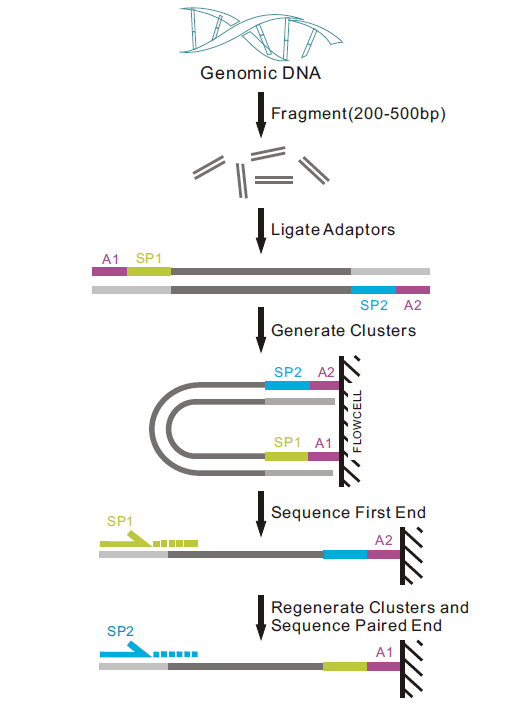
\includegraphics[width=0.5\linewidth]{static/images/library} 

}

\caption{全基因组重测序实验建库流程}\label{fig:library-plot}
\end{figure}

\hypertarget{ux751fux7269ux4fe1ux606fux5206ux6790ux6d41ux7a0b}{%
\subsection{生物信息分析流程}\label{ux751fux7269ux4fe1ux606fux5206ux6790ux6d41ux7a0b}}

在Illumina NovaSeq\(\rm{^{TM}}\)测序数据(Raw Data)下机之后,对下机数据进行质量控制,过滤其中低质量的数据,获得高质量的数据(Clean Data)。利用BWA-MEME软件(Jung and Han 2022)将Clean Data比对到参考基因组序列上,获得序列的位置归属(即BAM文件)。利用GATK软件(McKenna A \emph{et al.} 2010)的Best Practices流程对BAM文件进行校正,并进行SNP标记的检测。利用SNPEff软件(Cingolani \emph{et al.} 2012)和参考基因组的基因预测信息进行变异功能注释,得到SNP的功能注释信息。基于获得的SNP分子标记进一步进行图谱构建及QTL定位分析。分析流程见图\ref{fig:pipeline-plot}。

\begin{figure}[H]

{\centering 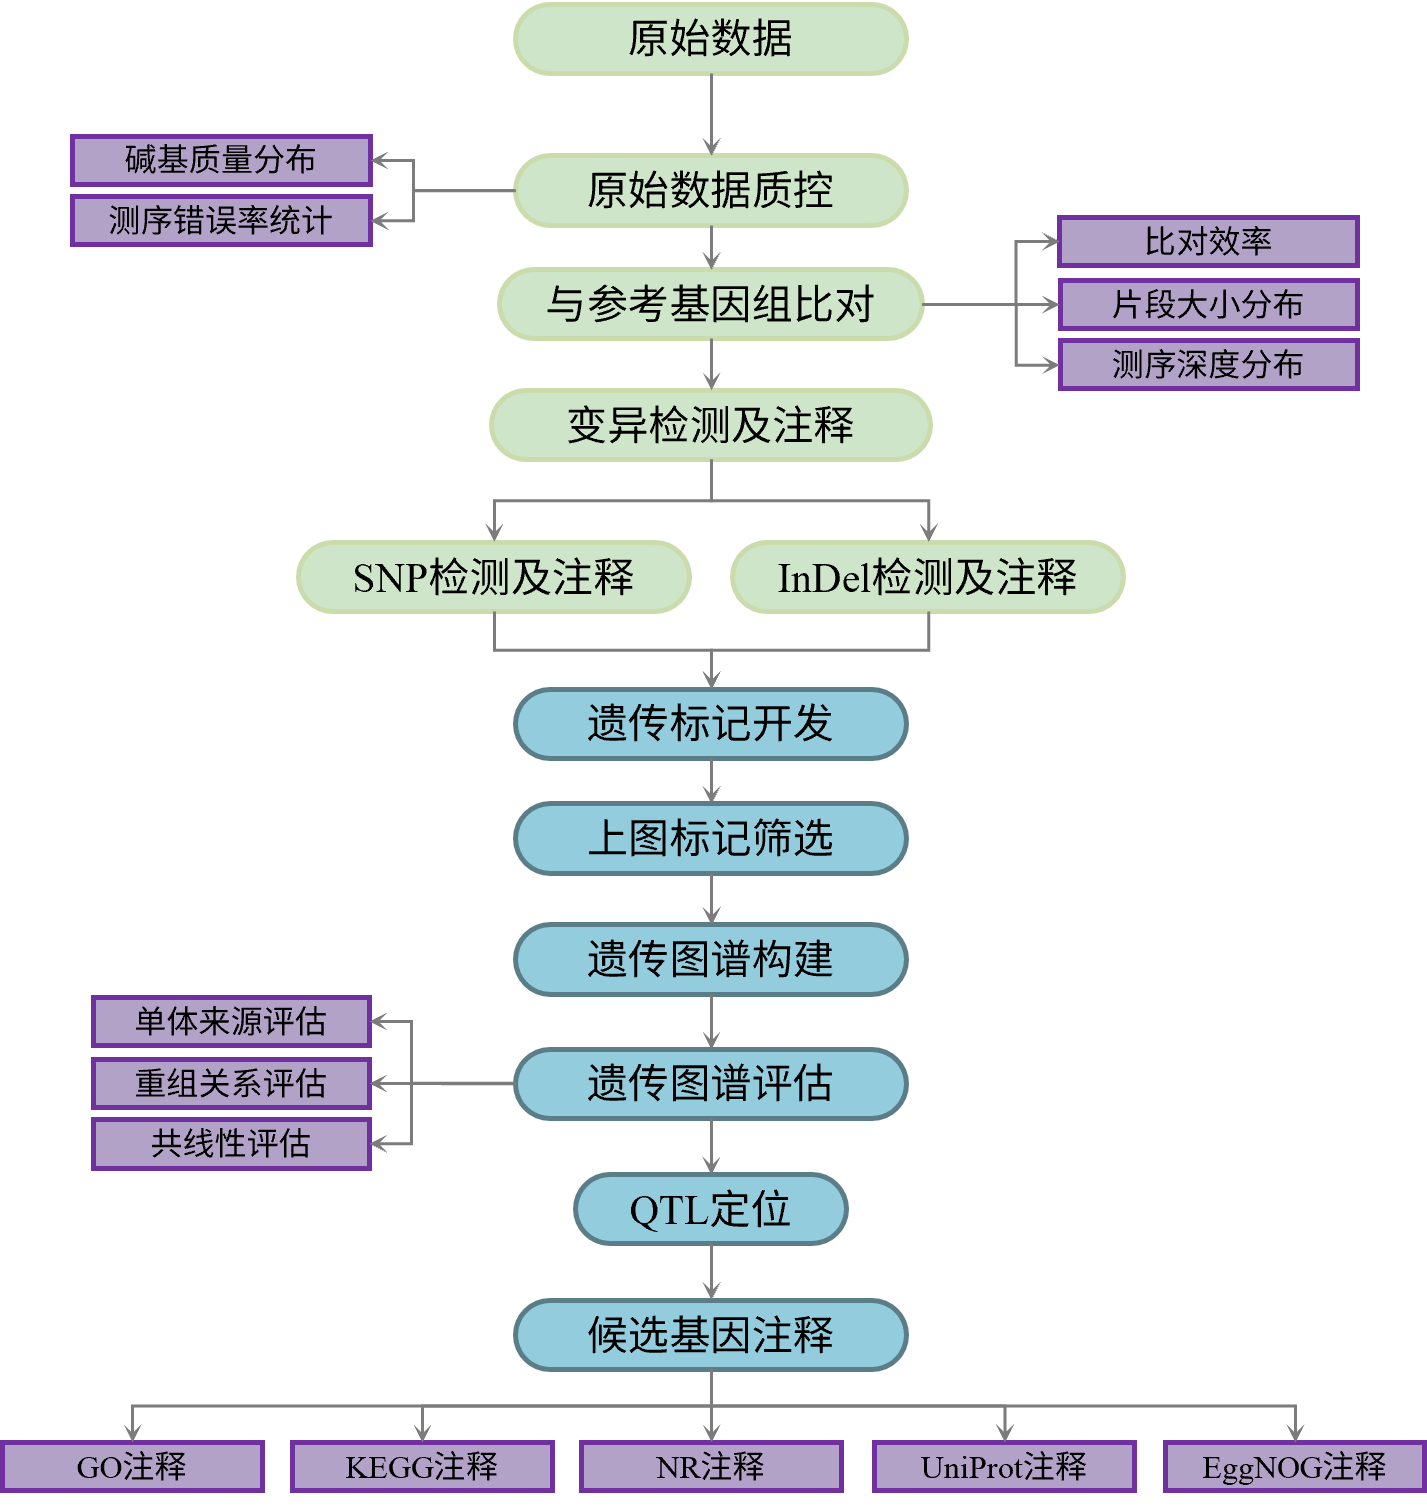
\includegraphics[width=1\linewidth]{static/images/pipeline} 

}

\caption{遗传图谱构建流程图}\label{fig:pipeline-plot}
\end{figure}

\clearpage

\clearpage

\hypertarget{ux751fux7269ux4fe1ux606fux5b66ux5206ux6790ux65b9ux6cd5ux548cux7ed3ux679c}{%
\section{生物信息学分析方法和结果}\label{ux751fux7269ux4fe1ux606fux5b66ux5206ux6790ux65b9ux6cd5ux548cux7ed3ux679c}}

\hypertarget{ux539fux59cbux6570ux636eux8d28ux63a7ux548cux8fc7ux6ee4}{%
\subsection{原始数据质控和过滤}\label{ux539fux59cbux6570ux636eux8d28ux63a7ux548cux8fc7ux6ee4}}

\hypertarget{ux539fux59cbux6d4bux5e8fux6570ux636eux8bf4ux660e}{%
\subsubsection{原始测序数据说明}\label{ux539fux59cbux6d4bux5e8fux6570ux636eux8bf4ux660e}}

为方便测序数据的分析、发布和共享,Illumina NovaSeq\(\rm{^{TM}}\)平台测序得到的原始图像数据经过Base Calling转化为序列数据,得到最原始的测序数据文件。一般原始数据利用FASTQ格式进行储存。FASTQ格式文件可记录所测读段(Read)的碱基及其质量分数。如图\ref{fig:fastq-plot}所示,FASTQ格式以测序读段为单位进行存储,每条Reads在FASTQ格式文件中占四行,其中第一行和第三行由文件识别标志(Sequence Identifiers)和读段名(ID)组成(第一行以``@''开头而第三行以``+''开头;第三行中ID可以省略,但``+''不能省略),第二行为碱基序列,第四行为对应位置碱基的测序质量分数。

\begin{figure}[H]

{\centering 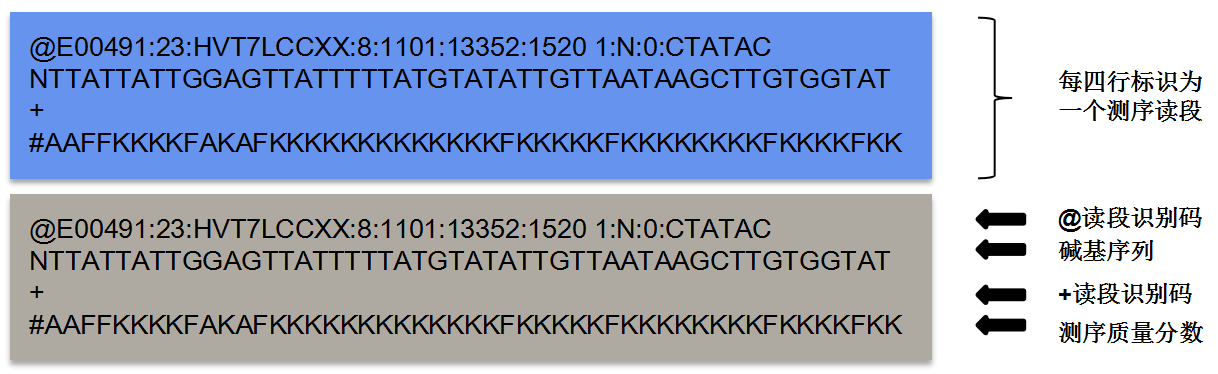
\includegraphics[width=0.5\linewidth]{static/images/fastq} 

}

\caption{读段FASTQ数据格式示例}\label{fig:fastq-plot}
\end{figure}

Illumina NovaSeq\(\rm{^{TM}}\)测序仪一个Run有2个Flowcell,一个Flowcell中包含8个Lane,其中一个Lane包含2列,每一列又包含60个Tile,每一个Tile又会包含不同的Cluster,其产生的测序文件识别标志(Sequence Identifiers)中的详细信息如表\ref{tab:fastq-details}所示:

\begin{longtable}[t]{ll}
\caption{\label{tab:fastq-details}测序文件识别标志详细信息}\\
\toprule
标识 & 英文描述\\
\midrule
\endfirsthead
\caption[]{\label{tab:fastq-details}测序文件识别标志详细信息 (续)}\\
\toprule
标识 & 英文描述\\
\midrule
\endhead
\hline
\endfoot
\bottomrule
\endlastfoot
\cellcolor{gray!6}{E00491} & \cellcolor{gray!6}{Unique instrument name}\\
 
23 & Run ID\\
 
\cellcolor{gray!6}{HVT7LCCXX} & \cellcolor{gray!6}{Flowcell ID}\\
 
8 & Flowcell lane\\
 
\cellcolor{gray!6}{1101} & \cellcolor{gray!6}{Tile number within the flowcell lane}\\
 
13352 & 'x'-coordinate of the cluster within the tile\\
 
\cellcolor{gray!6}{1520} & \cellcolor{gray!6}{'y'-coordinate of the cluster within the tile}\\
 
1 & Member of a pair, 1 or 2 (paired-end or mate-pair reads only)\\
 
\cellcolor{gray!6}{N} & \cellcolor{gray!6}{Y if the read fails filter (read is bad), N otherwise}\\
 
0 & 0 when none of the control bits are on, otherwise it is an even number\\
 
\cellcolor{gray!6}{CTATAC} & \cellcolor{gray!6}{Index sequence}\\*
\end{longtable}

Reads的质量分数以不同的字符来表示,其中每个字符对应的ASCII值减去33,即为对应的测序质量值。一般地,碱基质量从0到40,对应的ASCII码为从``!''(0+33)到``I''(40+33),碱基质量越大,可信度越高。用E表示测序错误率,用Q表示Illumina NovaSeq\(\rm{^{TM}}\)的碱基质量值,则有下列关系:

\[ Q = -10log_{10}(E) \]

\begin{longtable}[t]{lrl}
\caption{\label{tab:err-details}测序错误率与测序质量值简明对应关系}\\
\toprule
测序错误率 & 测序质量值 & 对应 ASCII 码\\
\midrule
\endfirsthead
\caption[]{\label{tab:err-details}测序错误率与测序质量值简明对应关系 (续)}\\
\toprule
测序错误率 & 测序质量值 & 对应 ASCII 码\\
\midrule
\endhead
\hline
\endfoot
\bottomrule
\endlastfoot
\cellcolor{gray!6}{5\%} & \cellcolor{gray!6}{13} & \cellcolor{gray!6}{.}\\
 
1\% & 20 & 5\\
 
\cellcolor{gray!6}{0.1\%} & \cellcolor{gray!6}{30} & \cellcolor{gray!6}{?}\\
 
0.01\% & 40 & I\\*
\end{longtable}

Illumina测序属于第二代测序技术,单次运行能产生数百万级的Reads,如此海量的数据无法逐个展示每条Read的质量情况;运用统计学的方法,对所有测序Reads的每个Cycle进行碱基分布和质量波动的统计,可以从宏观上直观地反映出样本的测序质量和文库构建质量。我们针对每一个样本的原始测序数据进行测序相关质量评估,包括A/T/G/C碱基含量分布统计和碱基错误率分布统计。

\begin{longtable}[t]{lllll}
\caption{\label{tab:rawdata-table}产出数据统计结果}\\
\toprule
Sample ID & Raw Reads & Raw Bases (bp) & Raw GC (\%) & Raw Q30 (\%)\\
\midrule
\endfirsthead
\caption[]{\label{tab:rawdata-table}产出数据统计结果 (续)}\\
\toprule
Sample ID & Raw Reads & Raw Bases (bp) & Raw GC (\%) & Raw Q30 (\%)\\
\midrule
\endhead
\hline
\endfoot
\bottomrule
\multicolumn{5}{l}{\rule{0pt}{1em}\textit{注:}}\\
\multicolumn{5}{l}{\rule{0pt}{1em}Sample ID:样本编号;}\\
\multicolumn{5}{l}{\rule{0pt}{1em}Raw Reads:原始的Reads数;}\\
\multicolumn{5}{l}{\rule{0pt}{1em}Raw Bases (bp):原始测序数据总碱基数;}\\
\multicolumn{5}{l}{\rule{0pt}{1em}Raw GC (\%):原始测序数据中的GC碱基占所有碱基的比例;}\\
\multicolumn{5}{l}{\rule{0pt}{1em}Raw Q30 (\%):原始测序数据中质量值大于或等于30的碱基所占百分比。}\\
\endlastfoot
\cellcolor{gray!6}{FJMS} & \cellcolor{gray!6}{45,151,054} & \cellcolor{gray!6}{6,762,077,180} & \cellcolor{gray!6}{34.58} & \cellcolor{gray!6}{100.00}\\
 
H1 & 10,155,004 & 1,520,723,054 & 35.31 & 100.00\\
 
\cellcolor{gray!6}{H3} & \cellcolor{gray!6}{6,398,326} & \cellcolor{gray!6}{958,307,115} & \cellcolor{gray!6}{34.41} & \cellcolor{gray!6}{100.00}\\
 
H3J1 & 8,901,064 & 1,333,225,139 & 35.03 & 100.00\\
 
\cellcolor{gray!6}{H3J2} & \cellcolor{gray!6}{9,306,464} & \cellcolor{gray!6}{1,393,857,776} & \cellcolor{gray!6}{35.09} & \cellcolor{gray!6}{100.00}\\
 
H3J3 & 7,620,842 & 1,141,364,534 & 34.88 & 100.00\\
 
\cellcolor{gray!6}{H3J4} & \cellcolor{gray!6}{8,923,024} & \cellcolor{gray!6}{1,336,401,487} & \cellcolor{gray!6}{35.90} & \cellcolor{gray!6}{100.00}\\
 
H3J5 & 11,688,162 & 1,750,688,952 & 35.01 & 100.00\\
 
\cellcolor{gray!6}{H3J6} & \cellcolor{gray!6}{10,244,740} & \cellcolor{gray!6}{1,534,416,755} & \cellcolor{gray!6}{34.61} & \cellcolor{gray!6}{100.00}\\
 
H3J7 & 9,379,938 & 1,404,638,088 & 34.47 & 100.00\\
 
\cellcolor{gray!6}{H3J8} & \cellcolor{gray!6}{8,680,212} & \cellcolor{gray!6}{1,300,238,221} & \cellcolor{gray!6}{34.76} & \cellcolor{gray!6}{100.00}\\
 
H3J10 & 8,599,024 & 1,287,741,769 & 34.98 & 100.00\\
 
\cellcolor{gray!6}{H3J11} & \cellcolor{gray!6}{8,615,504} & \cellcolor{gray!6}{1,290,235,870} & \cellcolor{gray!6}{34.98} & \cellcolor{gray!6}{100.00}\\
 
H3J12 & 9,525,568 & 1,426,439,169 & 34.79 & 100.00\\
 
\cellcolor{gray!6}{H3J13} & \cellcolor{gray!6}{8,852,826} & \cellcolor{gray!6}{1,326,006,951} & \cellcolor{gray!6}{34.65} & \cellcolor{gray!6}{100.00}\\
 
H3J14 & 9,503,698 & 1,423,373,983 & 34.85 & 100.00\\
 
\cellcolor{gray!6}{H3J15} & \cellcolor{gray!6}{8,971,650} & \cellcolor{gray!6}{1,343,601,836} & \cellcolor{gray!6}{34.40} & \cellcolor{gray!6}{100.00}\\
 
H3J16 & 11,082,252 & 1,659,832,584 & 34.68 & 100.00\\
 
\cellcolor{gray!6}{H3J18} & \cellcolor{gray!6}{8,503,574} & \cellcolor{gray!6}{1,273,426,048} & \cellcolor{gray!6}{34.74} & \cellcolor{gray!6}{100.00}\\
 
H3J19 & 8,429,026 & 1,262,104,630 & 34.66 & 100.00\\
 
\cellcolor{gray!6}{H3J20} & \cellcolor{gray!6}{9,607,148} & \cellcolor{gray!6}{1,438,941,535} & \cellcolor{gray!6}{34.28} & \cellcolor{gray!6}{100.00}\\
 
H3J21 & 7,721,986 & 1,156,413,604 & 35.06 & 100.00\\
 
\cellcolor{gray!6}{H3J22} & \cellcolor{gray!6}{9,075,498} & \cellcolor{gray!6}{1,359,104,642} & \cellcolor{gray!6}{35.26} & \cellcolor{gray!6}{100.00}\\
 
H3J23 & 6,731,090 & 1,007,878,505 & 34.96 & 100.00\\
 
\cellcolor{gray!6}{H4} & \cellcolor{gray!6}{9,515,152} & \cellcolor{gray!6}{1,425,017,606} & \cellcolor{gray!6}{35.23} & \cellcolor{gray!6}{100.00}\\
 
H5 & 8,783,882 & 1,315,594,927 & 34.89 & 100.00\\
 
\cellcolor{gray!6}{H8} & \cellcolor{gray!6}{7,871,818} & \cellcolor{gray!6}{1,179,088,243} & \cellcolor{gray!6}{34.81} & \cellcolor{gray!6}{100.00}\\
 
H9 & 7,927,218 & 1,187,184,778 & 34.87 & 100.00\\
 
\cellcolor{gray!6}{H10} & \cellcolor{gray!6}{10,371,526} & \cellcolor{gray!6}{1,553,541,189} & \cellcolor{gray!6}{34.55} & \cellcolor{gray!6}{100.00}\\
 
H11 & 10,027,798 & 1,501,571,220 & 35.06 & 100.00\\
 
\cellcolor{gray!6}{H13} & \cellcolor{gray!6}{10,203,598} & \cellcolor{gray!6}{1,528,513,658} & \cellcolor{gray!6}{34.75} & \cellcolor{gray!6}{100.00}\\
 
H15 & 9,077,466 & 1,359,198,281 & 35.52 & 100.00\\
 
\cellcolor{gray!6}{H16} & \cellcolor{gray!6}{10,074,934} & \cellcolor{gray!6}{1,508,644,424} & \cellcolor{gray!6}{34.71} & \cellcolor{gray!6}{100.00}\\
 
H17 & 8,364,552 & 1,252,475,762 & 34.55 & 100.00\\
 
\cellcolor{gray!6}{H18} & \cellcolor{gray!6}{10,597,118} & \cellcolor{gray!6}{1,586,685,911} & \cellcolor{gray!6}{34.40} & \cellcolor{gray!6}{100.00}\\
 
H20 & 8,717,102 & 1,305,164,494 & 34.89 & 100.00\\
 
\cellcolor{gray!6}{H21} & \cellcolor{gray!6}{8,768,526} & \cellcolor{gray!6}{1,313,089,189} & \cellcolor{gray!6}{34.87} & \cellcolor{gray!6}{100.00}\\
 
H22 & 10,611,832 & 1,589,518,145 & 34.29 & 100.00\\
 
\cellcolor{gray!6}{H23} & \cellcolor{gray!6}{7,582,404} & \cellcolor{gray!6}{1,135,519,100} & \cellcolor{gray!6}{34.52} & \cellcolor{gray!6}{100.00}\\
 
H25 & 7,623,418 & 1,141,627,887 & 34.80 & 100.00\\
 
\cellcolor{gray!6}{H26} & \cellcolor{gray!6}{9,024,440} & \cellcolor{gray!6}{1,351,395,898} & \cellcolor{gray!6}{35.02} & \cellcolor{gray!6}{100.00}\\
 
H28 & 10,535,954 & 1,578,215,020 & 34.70 & 100.00\\
 
\cellcolor{gray!6}{H30} & \cellcolor{gray!6}{9,513,590} & \cellcolor{gray!6}{1,424,738,234} & \cellcolor{gray!6}{34.46} & \cellcolor{gray!6}{100.00}\\
 
H31 & 9,828,554 & 1,472,232,259 & 34.40 & 100.00\\
 
\cellcolor{gray!6}{H36} & \cellcolor{gray!6}{11,699,752} & \cellcolor{gray!6}{1,752,490,161} & \cellcolor{gray!6}{34.82} & \cellcolor{gray!6}{100.00}\\
 
H37 & 8,149,110 & 1,220,434,722 & 34.52 & 100.00\\
 
\cellcolor{gray!6}{H38} & \cellcolor{gray!6}{10,389,144} & \cellcolor{gray!6}{1,555,769,286} & \cellcolor{gray!6}{34.54} & \cellcolor{gray!6}{100.00}\\
 
H39 & 7,708,506 & 1,154,643,031 & 34.82 & 100.00\\
 
\cellcolor{gray!6}{H41} & \cellcolor{gray!6}{12,309,124} & \cellcolor{gray!6}{1,843,598,046} & \cellcolor{gray!6}{34.70} & \cellcolor{gray!6}{100.00}\\
 
H42 & 10,378,202 & 1,553,781,871 & 34.58 & 100.00\\
 
\cellcolor{gray!6}{H43} & \cellcolor{gray!6}{8,385,286} & \cellcolor{gray!6}{1,256,056,917} & \cellcolor{gray!6}{35.03} & \cellcolor{gray!6}{100.00}\\
 
H44 & 10,724,812 & 1,606,372,394 & 34.79 & 100.00\\
 
\cellcolor{gray!6}{H45} & \cellcolor{gray!6}{9,433,246} & \cellcolor{gray!6}{1,412,686,257} & \cellcolor{gray!6}{34.83} & \cellcolor{gray!6}{100.00}\\
 
H46 & 8,059,902 & 1,206,938,916 & 34.75 & 100.00\\
 
\cellcolor{gray!6}{H47} & \cellcolor{gray!6}{9,245,140} & \cellcolor{gray!6}{1,384,656,039} & \cellcolor{gray!6}{34.77} & \cellcolor{gray!6}{100.00}\\
 
H49 & 8,647,976 & 1,295,292,633 & 34.86 & 100.00\\
 
\cellcolor{gray!6}{H50} & \cellcolor{gray!6}{9,209,082} & \cellcolor{gray!6}{1,379,348,066} & \cellcolor{gray!6}{34.22} & \cellcolor{gray!6}{100.00}\\
 
H51 & 8,999,432 & 1,347,653,855 & 34.81 & 100.00\\
 
\cellcolor{gray!6}{H52} & \cellcolor{gray!6}{9,971,156} & \cellcolor{gray!6}{1,493,435,918} & \cellcolor{gray!6}{34.57} & \cellcolor{gray!6}{100.00}\\
 
H54 & 8,140,806 & 1,219,067,465 & 34.95 & 100.00\\
 
\cellcolor{gray!6}{H55} & \cellcolor{gray!6}{11,373,972} & \cellcolor{gray!6}{1,703,591,590} & \cellcolor{gray!6}{34.92} & \cellcolor{gray!6}{100.00}\\
 
H56 & 8,752,638 & 1,310,956,477 & 34.74 & 100.00\\
 
\cellcolor{gray!6}{H58} & \cellcolor{gray!6}{7,937,916} & \cellcolor{gray!6}{1,188,802,333} & \cellcolor{gray!6}{34.55} & \cellcolor{gray!6}{100.00}\\
 
H59 & 8,752,856 & 1,310,802,940 & 34.93 & 100.00\\
 
\cellcolor{gray!6}{H61} & \cellcolor{gray!6}{7,701,034} & \cellcolor{gray!6}{1,153,218,387} & \cellcolor{gray!6}{34.85} & \cellcolor{gray!6}{100.00}\\
 
H62 & 9,037,514 & 1,353,273,357 & 34.77 & 100.00\\
 
\cellcolor{gray!6}{H63} & \cellcolor{gray!6}{9,694,688} & \cellcolor{gray!6}{1,452,103,613} & \cellcolor{gray!6}{34.62} & \cellcolor{gray!6}{100.00}\\
 
H64 & 7,614,940 & 1,139,911,971 & 34.87 & 100.00\\
 
\cellcolor{gray!6}{H70} & \cellcolor{gray!6}{9,560,600} & \cellcolor{gray!6}{1,431,845,110} & \cellcolor{gray!6}{34.51} & \cellcolor{gray!6}{100.00}\\
 
H74 & 8,542,670 & 1,279,257,117 & 34.67 & 100.00\\
 
\cellcolor{gray!6}{H76} & \cellcolor{gray!6}{8,614,514} & \cellcolor{gray!6}{1,289,687,778} & \cellcolor{gray!6}{35.26} & \cellcolor{gray!6}{100.00}\\
 
H77 & 8,845,346 & 1,324,653,193 & 34.81 & 100.00\\
 
\cellcolor{gray!6}{H80} & \cellcolor{gray!6}{8,075,084} & \cellcolor{gray!6}{1,209,394,226} & \cellcolor{gray!6}{35.03} & \cellcolor{gray!6}{100.00}\\
 
H81 & 9,905,376 & 1,483,069,380 & 34.31 & 100.00\\
 
\cellcolor{gray!6}{H82} & \cellcolor{gray!6}{8,330,764} & \cellcolor{gray!6}{1,247,241,967} & \cellcolor{gray!6}{34.65} & \cellcolor{gray!6}{100.00}\\
 
H83 & 10,059,616 & 1,505,721,894 & 34.98 & 100.00\\
 
\cellcolor{gray!6}{H84} & \cellcolor{gray!6}{9,406,078} & \cellcolor{gray!6}{1,408,826,710} & \cellcolor{gray!6}{34.82} & \cellcolor{gray!6}{100.00}\\
 
H85 & 9,198,730 & 1,377,284,469 & 34.95 & 100.00\\
 
\cellcolor{gray!6}{H87} & \cellcolor{gray!6}{8,920,732} & \cellcolor{gray!6}{1,335,589,305} & \cellcolor{gray!6}{35.23} & \cellcolor{gray!6}{100.00}\\
 
H89 & 8,293,480 & 1,242,253,277 & 34.46 & 100.00\\
 
\cellcolor{gray!6}{H91} & \cellcolor{gray!6}{7,435,980} & \cellcolor{gray!6}{1,113,669,081} & \cellcolor{gray!6}{34.60} & \cellcolor{gray!6}{100.00}\\
 
H92 & 9,856,270 & 1,476,352,197 & 34.81 & 100.00\\
 
\cellcolor{gray!6}{H93} & \cellcolor{gray!6}{7,630,890} & \cellcolor{gray!6}{1,142,655,506} & \cellcolor{gray!6}{34.64} & \cellcolor{gray!6}{100.00}\\
 
H94 & 12,243,364 & 1,833,998,581 & 35.53 & 100.00\\
 
\cellcolor{gray!6}{H95} & \cellcolor{gray!6}{8,461,766} & \cellcolor{gray!6}{1,266,493,753} & \cellcolor{gray!6}{34.68} & \cellcolor{gray!6}{100.00}\\
 
H96 & 9,307,888 & 1,394,029,728 & 34.94 & 100.00\\
 
\cellcolor{gray!6}{H97} & \cellcolor{gray!6}{8,315,308} & \cellcolor{gray!6}{1,245,382,415} & \cellcolor{gray!6}{35.05} & \cellcolor{gray!6}{100.00}\\
 
H100 & 10,394,320 & 1,556,674,380 & 34.63 & 100.00\\
 
\cellcolor{gray!6}{H102} & \cellcolor{gray!6}{9,891,700} & \cellcolor{gray!6}{1,481,070,979} & \cellcolor{gray!6}{34.68} & \cellcolor{gray!6}{100.00}\\
 
H104 & 10,363,396 & 1,552,553,098 & 34.58 & 100.00\\
 
\cellcolor{gray!6}{H105} & \cellcolor{gray!6}{7,443,108} & \cellcolor{gray!6}{1,114,588,155} & \cellcolor{gray!6}{35.01} & \cellcolor{gray!6}{100.00}\\
 
H106 & 9,370,378 & 1,403,497,904 & 34.32 & 100.00\\
 
\cellcolor{gray!6}{H108} & \cellcolor{gray!6}{8,313,452} & \cellcolor{gray!6}{1,244,916,936} & \cellcolor{gray!6}{34.20} & \cellcolor{gray!6}{100.00}\\
 
H109 & 8,442,638 & 1,264,291,681 & 34.86 & 100.00\\
 
\cellcolor{gray!6}{H112} & \cellcolor{gray!6}{12,163,126} & \cellcolor{gray!6}{1,821,886,417} & \cellcolor{gray!6}{35.56} & \cellcolor{gray!6}{100.00}\\
 
H113 & 10,585,108 & 1,585,187,080 & 34.97 & 100.00\\
 
\cellcolor{gray!6}{H115} & \cellcolor{gray!6}{11,786,208} & \cellcolor{gray!6}{1,764,929,603} & \cellcolor{gray!6}{34.71} & \cellcolor{gray!6}{100.00}\\
 
H116 & 9,335,174 & 1,398,177,236 & 35.23 & 100.00\\
 
\cellcolor{gray!6}{H117} & \cellcolor{gray!6}{10,474,574} & \cellcolor{gray!6}{1,568,944,541} & \cellcolor{gray!6}{34.78} & \cellcolor{gray!6}{100.00}\\
 
H120 & 8,282,458 & 1,240,217,362 & 33.96 & 100.00\\
 
\cellcolor{gray!6}{H121} & \cellcolor{gray!6}{8,978,486} & \cellcolor{gray!6}{1,344,812,205} & \cellcolor{gray!6}{34.74} & \cellcolor{gray!6}{100.00}\\
 
H124 & 7,749,802 & 1,160,469,743 & 34.46 & 100.00\\
 
\cellcolor{gray!6}{H127} & \cellcolor{gray!6}{8,139,828} & \cellcolor{gray!6}{1,219,020,585} & \cellcolor{gray!6}{34.80} & \cellcolor{gray!6}{100.00}\\
 
H128 & 9,772,568 & 1,463,703,697 & 34.51 & 100.00\\
 
\cellcolor{gray!6}{H129} & \cellcolor{gray!6}{6,886,274} & \cellcolor{gray!6}{1,031,065,447} & \cellcolor{gray!6}{34.67} & \cellcolor{gray!6}{100.00}\\
 
H132 & 9,509,644 & 1,424,134,930 & 34.93 & 100.00\\
 
\cellcolor{gray!6}{H135} & \cellcolor{gray!6}{8,083,578} & \cellcolor{gray!6}{1,210,412,745} & \cellcolor{gray!6}{34.52} & \cellcolor{gray!6}{100.00}\\
 
H137 & 6,493,300 & 972,062,816 & 36.32 & 100.00\\
 
\cellcolor{gray!6}{H138} & \cellcolor{gray!6}{9,240,716} & \cellcolor{gray!6}{1,383,657,705} & \cellcolor{gray!6}{34.70} & \cellcolor{gray!6}{100.00}\\
 
H140 & 8,047,410 & 1,205,076,199 & 34.63 & 100.00\\
 
\cellcolor{gray!6}{H142} & \cellcolor{gray!6}{6,249,442} & \cellcolor{gray!6}{935,855,185} & \cellcolor{gray!6}{34.90} & \cellcolor{gray!6}{100.00}\\
 
H143 & 9,277,392 & 1,388,765,316 & 34.79 & 100.00\\
 
\cellcolor{gray!6}{H144} & \cellcolor{gray!6}{7,824,922} & \cellcolor{gray!6}{1,171,907,299} & \cellcolor{gray!6}{34.63} & \cellcolor{gray!6}{100.00}\\
 
H145 & 9,306,654 & 1,393,677,385 & 35.17 & 100.00\\
 
\cellcolor{gray!6}{H146} & \cellcolor{gray!6}{7,289,368} & \cellcolor{gray!6}{1,091,741,105} & \cellcolor{gray!6}{34.88} & \cellcolor{gray!6}{100.00}\\
 
H148 & 6,599,092 & 988,369,703 & 34.67 & 100.00\\
 
\cellcolor{gray!6}{H149} & \cellcolor{gray!6}{8,072,010} & \cellcolor{gray!6}{1,208,867,327} & \cellcolor{gray!6}{34.51} & \cellcolor{gray!6}{100.00}\\
 
H150 & 10,151,600 & 1,520,370,257 & 34.34 & 100.00\\
 
\cellcolor{gray!6}{H151} & \cellcolor{gray!6}{10,397,040} & \cellcolor{gray!6}{1,557,370,608} & \cellcolor{gray!6}{34.63} & \cellcolor{gray!6}{100.00}\\
 
H152 & 8,218,834 & 1,230,892,418 & 35.35 & 100.00\\
 
\cellcolor{gray!6}{H157} & \cellcolor{gray!6}{9,946,306} & \cellcolor{gray!6}{1,489,389,199} & \cellcolor{gray!6}{35.03} & \cellcolor{gray!6}{100.00}\\
 
H158 & 8,436,628 & 1,263,161,223 & 35.51 & 100.00\\
 
\cellcolor{gray!6}{H159} & \cellcolor{gray!6}{9,089,804} & \cellcolor{gray!6}{1,361,290,878} & \cellcolor{gray!6}{35.26} & \cellcolor{gray!6}{100.00}\\
 
H160 & 8,389,996 & 1,256,505,138 & 36.48 & 100.00\\
 
\cellcolor{gray!6}{H161} & \cellcolor{gray!6}{10,163,162} & \cellcolor{gray!6}{1,522,304,934} & \cellcolor{gray!6}{35.01} & \cellcolor{gray!6}{100.00}\\
 
H162 & 10,948,948 & 1,639,300,602 & 34.90 & 100.00\\
 
\cellcolor{gray!6}{H164} & \cellcolor{gray!6}{11,545,164} & \cellcolor{gray!6}{1,729,192,162} & \cellcolor{gray!6}{34.82} & \cellcolor{gray!6}{100.00}\\
 
H166 & 9,672,324 & 1,448,835,471 & 34.89 & 100.00\\
 
\cellcolor{gray!6}{H167} & \cellcolor{gray!6}{8,970,604} & \cellcolor{gray!6}{1,343,670,722} & \cellcolor{gray!6}{36.39} & \cellcolor{gray!6}{100.00}\\
 
H168 & 9,559,198 & 1,431,700,401 & 34.88 & 100.00\\
 
\cellcolor{gray!6}{H169} & \cellcolor{gray!6}{7,990,816} & \cellcolor{gray!6}{1,196,646,811} & \cellcolor{gray!6}{34.57} & \cellcolor{gray!6}{100.00}\\
 
H170 & 7,951,082 & 1,191,076,748 & 34.92 & 100.00\\
 
\cellcolor{gray!6}{H171} & \cellcolor{gray!6}{10,698,960} & \cellcolor{gray!6}{1,602,615,056} & \cellcolor{gray!6}{34.92} & \cellcolor{gray!6}{100.00}\\
 
H172 & 6,998,498 & 1,048,277,174 & 36.46 & 100.00\\
 
\cellcolor{gray!6}{H173} & \cellcolor{gray!6}{7,296,598} & \cellcolor{gray!6}{1,092,804,407} & \cellcolor{gray!6}{35.15} & \cellcolor{gray!6}{100.00}\\
 
H174 & 9,095,666 & 1,362,552,895 & 35.12 & 100.00\\
 
\cellcolor{gray!6}{H175} & \cellcolor{gray!6}{8,087,960} & \cellcolor{gray!6}{1,211,553,230} & \cellcolor{gray!6}{34.39} & \cellcolor{gray!6}{100.00}\\
 
H176 & 10,435,718 & 1,563,061,811 & 35.09 & 100.00\\
 
\cellcolor{gray!6}{H177} & \cellcolor{gray!6}{7,247,366} & \cellcolor{gray!6}{1,085,315,692} & \cellcolor{gray!6}{34.20} & \cellcolor{gray!6}{100.00}\\
 
H178 & 8,523,520 & 1,276,548,718 & 35.07 & 100.00\\
 
\cellcolor{gray!6}{H179} & \cellcolor{gray!6}{7,408,978} & \cellcolor{gray!6}{1,109,624,905} & \cellcolor{gray!6}{34.88} & \cellcolor{gray!6}{100.00}\\
 
MJ5 & 44,209,662 & 6,620,859,826 & 35.50 & 100.00\\*
\end{longtable}

\hypertarget{ux6d4bux5e8fux78b1ux57faux542bux91cfux5206ux5e03ux7edfux8ba1}{%
\subsubsection{测序碱基含量分布统计}\label{ux6d4bux5e8fux78b1ux57faux542bux91cfux5206ux5e03ux7edfux8ba1}}

碱基含量分布检查一般用于检测有无 A 与 T、G 与 C 分离现象。鉴于序列的随机性和碱基互补配对的原则,理论上每个测序循环上的 GC 含量相等、AT 含量相等,且在整个测序过程基本稳定不变,呈水平线。N 为测序仪无法判断的碱基类型。

在实际测序中,首先会将文库 DNA 模板固定到芯片上,使每个 DNA 分子形成一个簇,即一个测序位点,在固定过程中极少量的簇与簇之间物理位置会发生重叠。测序时仪器首先通过前 4 轮测序循环对这些重叠的点进行分析和识别,将这些重叠点位置分开,保证每个点测到的是一个 DNA 分子,因此前几个碱基的错误率可能偏高、碱基含量可能存在着一定波动,属于正常情况,后续的数据质控会对此进行过滤。

本项目中样品的碱基含量分布图如图\ref{fig:rawbase-plot}所示。

\begin{figure}[H]

{\centering \includegraphics[width=0.5\linewidth]{../../../../../../../../../../../ilustre/isanger_workspaceWgsV4/20240105/WgsV4_uk0k_1ujkihog35qgqe6s1vpf1m/output/tmp/01.fastq_qc/json/FJMS.raw.base} 

}

\caption{样本碱基组成分布图}\label{fig:rawbase-plot}
\end{figure}

\begin{quote}
\textbf{注:}横坐标是Reads碱基坐标,坐标表示Reads上从5'到3'端依次碱基的排列;纵坐标是所有Reads在该测序位置A、C、G、T、N碱基分别占的百分比,不同碱基用不同颜色表示。序列的起始位置与测序的引物接头相连,因此A、C、G、T在起始端会有所波动,后面会趋于稳定。模糊碱基N所占比例越低,说明未知碱基越少,测序样本受系统AT偏好影响越小。虚线之前为Read1的统计,虚线之后为Read2的统计结果。
\end{quote}

\hypertarget{ux6d4bux5e8fux78b1ux57faux9519ux8befux7387ux5206ux5e03ux7edfux8ba1}{%
\subsubsection{测序碱基错误率分布统计}\label{ux6d4bux5e8fux78b1ux57faux9519ux8befux7387ux5206ux5e03ux7edfux8ba1}}

测序错误率会随着测序序列长度的增加而升高,这是由测序过程中化学试剂的消耗导致的,另外,由于Illumina NovaSeq\(\rm{^{TM}}\)测序技术特点,测序片段前端几个Cycles和末端的错误率会偏高。本项目中所有样品的测序错误率分布图如图\ref{fig:rawqual-plot}所示。

\begin{figure}[H]

{\centering \includegraphics[width=0.5\linewidth]{../../../../../../../../../../../ilustre/isanger_workspaceWgsV4/20240105/WgsV4_uk0k_1ujkihog35qgqe6s1vpf1m/output/tmp/01.fastq_qc/json/FJMS.raw.qual} 

}

\caption{样本碱基错误率分布图}\label{fig:rawqual-plot}
\end{figure}

\begin{quote}
\textbf{注:}横坐标是Reads碱基坐标,表示Reads上从5'到3'端依次碱基的排列;纵坐标是所有Reads在该位点处碱基的平均错误率。前150bp为双端测序序列的第一端测序Reads的错误率分布情况,后150bp为另一端测序Reads的错误率分布情况。
\end{quote}

\hypertarget{ux539fux59cbux6d4bux5e8fux6570ux636eux8fc7ux6ee4}{%
\subsubsection{原始测序数据过滤}\label{ux539fux59cbux6d4bux5e8fux6570ux636eux8fc7ux6ee4}}

利用Illumina的建库测序平台,构建插入片段大小为350bp左右的测序文库,按照项目合同要求进行测序,对原始数据进行质量评估,具体步骤如下:

Step1:去除reads中的adapter序列;

Step2:剪切前去除5`端含有非AGCT的碱基;

Step3:修剪测序质量较低的reads末端(测序质量值小于Q20);

Step4:去除含N的比例达到10\%的reads;

Step5:舍弃去adapter及质量修剪后长度小于25bp的小片段。

对质量剪切后的数据分别进行测序Reads数、总碱基数、GC含量和Q30比例的统计,详细结果见表\ref{tab:cleanstat-table}:

\begin{longtable}[t]{lllll}
\caption{\label{tab:cleanstat-table}测序质量统计表}\\
\toprule
Sample ID & Clean Reads & Clean Bases (bp) & Clean GC (\%) & Clean Q30 (\%)\\
\midrule
\endfirsthead
\caption[]{\label{tab:cleanstat-table}测序质量统计表 (续)}\\
\toprule
Sample ID & Clean Reads & Clean Bases (bp) & Clean GC (\%) & Clean Q30 (\%)\\
\midrule
\endhead
\hline
\endfoot
\bottomrule
\multicolumn{5}{l}{\rule{0pt}{1em}\textit{注:}}\\
\multicolumn{5}{l}{\rule{0pt}{1em}Sample ID:样本编号;}\\
\multicolumn{5}{l}{\rule{0pt}{1em}Clean Reads:高质量的Reads数;}\\
\multicolumn{5}{l}{\rule{0pt}{1em}Clean Bases (bp):原始数据过滤后的高质量测序数据总碱基数;}\\
\multicolumn{5}{l}{\rule{0pt}{1em}Clean GC (\%):原始数据过滤后的GC碱基占所有碱基的比例;}\\
\multicolumn{5}{l}{\rule{0pt}{1em}Clean Q30 (\%):原始数据过滤后质量值大于或等于30的碱基所占百分比。}\\
\endlastfoot
\cellcolor{gray!6}{FJMS} & \cellcolor{gray!6}{45,140,754} & \cellcolor{gray!6}{6,755,813,140} & \cellcolor{gray!6}{34.60} & \cellcolor{gray!6}{100.00}\\
 
H1 & 10,152,458 & 1,519,220,837 & 35.32 & 100.00\\
 
\cellcolor{gray!6}{H3} & \cellcolor{gray!6}{6,396,978} & \cellcolor{gray!6}{957,446,321} & \cellcolor{gray!6}{34.50} & \cellcolor{gray!6}{100.00}\\
 
H3J1 & 8,899,098 & 1,331,964,178 & 35.06 & 100.00\\
 
\cellcolor{gray!6}{H3J2} & \cellcolor{gray!6}{9,304,530} & \cellcolor{gray!6}{1,392,643,281} & \cellcolor{gray!6}{35.10} & \cellcolor{gray!6}{100.00}\\
 
H3J3 & 7,618,952 & 1,140,183,157 & 34.91 & 100.00\\
 
\cellcolor{gray!6}{H3J4} & \cellcolor{gray!6}{8,920,620} & \cellcolor{gray!6}{1,335,092,618} & \cellcolor{gray!6}{35.94} & \cellcolor{gray!6}{100.00}\\
 
H3J5 & 11,685,584 & 1,749,070,423 & 35.03 & 100.00\\
 
\cellcolor{gray!6}{H3J6} & \cellcolor{gray!6}{10,242,554} & \cellcolor{gray!6}{1,533,022,227} & \cellcolor{gray!6}{34.64} & \cellcolor{gray!6}{100.00}\\
 
H3J7 & 9,377,556 & 1,403,192,664 & 34.50 & 100.00\\
 
\cellcolor{gray!6}{H3J8} & \cellcolor{gray!6}{8,678,384} & \cellcolor{gray!6}{1,299,148,818} & \cellcolor{gray!6}{34.79} & \cellcolor{gray!6}{100.00}\\
 
H3J10 & 8,597,232 & 1,286,639,442 & 35.03 & 100.00\\
 
\cellcolor{gray!6}{H3J11} & \cellcolor{gray!6}{8,613,384} & \cellcolor{gray!6}{1,288,954,551} & \cellcolor{gray!6}{35.00} & \cellcolor{gray!6}{100.00}\\
 
H3J12 & 9,523,128 & 1,424,969,262 & 34.81 & 100.00\\
 
\cellcolor{gray!6}{H3J13} & \cellcolor{gray!6}{8,850,952} & \cellcolor{gray!6}{1,324,778,893} & \cellcolor{gray!6}{34.68} & \cellcolor{gray!6}{100.00}\\
 
H3J14 & 9,501,708 & 1,422,104,065 & 34.87 & 100.00\\
 
\cellcolor{gray!6}{H3J15} & \cellcolor{gray!6}{8,969,904} & \cellcolor{gray!6}{1,342,414,615} & \cellcolor{gray!6}{34.41} & \cellcolor{gray!6}{100.00}\\
 
H3J16 & 11,079,606 & 1,658,191,242 & 34.70 & 100.00\\
 
\cellcolor{gray!6}{H3J18} & \cellcolor{gray!6}{8,501,838} & \cellcolor{gray!6}{1,272,289,549} & \cellcolor{gray!6}{34.78} & \cellcolor{gray!6}{100.00}\\
 
H3J19 & 8,426,934 & 1,260,826,271 & 34.66 & 100.00\\
 
\cellcolor{gray!6}{H3J20} & \cellcolor{gray!6}{9,605,180} & \cellcolor{gray!6}{1,437,693,473} & \cellcolor{gray!6}{34.31} & \cellcolor{gray!6}{100.00}\\
 
H3J21 & 7,720,030 & 1,155,204,662 & 35.08 & 100.00\\
 
\cellcolor{gray!6}{H3J22} & \cellcolor{gray!6}{9,073,194} & \cellcolor{gray!6}{1,357,634,556} & \cellcolor{gray!6}{35.28} & \cellcolor{gray!6}{100.00}\\
 
H3J23 & 6,729,490 & 1,006,932,657 & 35.00 & 100.00\\
 
\cellcolor{gray!6}{H4} & \cellcolor{gray!6}{9,512,958} & \cellcolor{gray!6}{1,423,696,890} & \cellcolor{gray!6}{35.26} & \cellcolor{gray!6}{100.00}\\
 
H5 & 8,782,104 & 1,314,442,505 & 34.92 & 100.00\\
 
\cellcolor{gray!6}{H8} & \cellcolor{gray!6}{7,870,052} & \cellcolor{gray!6}{1,177,999,125} & \cellcolor{gray!6}{34.83} & \cellcolor{gray!6}{100.00}\\
 
H9 & 7,925,408 & 1,186,046,129 & 34.88 & 100.00\\
 
\cellcolor{gray!6}{H10} & \cellcolor{gray!6}{10,369,304} & \cellcolor{gray!6}{1,552,147,216} & \cellcolor{gray!6}{34.58} & \cellcolor{gray!6}{100.00}\\
 
H11 & 10,025,526 & 1,500,127,440 & 35.11 & 100.00\\
 
\cellcolor{gray!6}{H13} & \cellcolor{gray!6}{10,201,542} & \cellcolor{gray!6}{1,527,224,016} & \cellcolor{gray!6}{34.79} & \cellcolor{gray!6}{100.00}\\
 
H15 & 9,075,662 & 1,358,064,963 & 35.55 & 100.00\\
 
\cellcolor{gray!6}{H16} & \cellcolor{gray!6}{10,072,608} & \cellcolor{gray!6}{1,507,245,286} & \cellcolor{gray!6}{34.74} & \cellcolor{gray!6}{100.00}\\
 
H17 & 8,362,594 & 1,251,292,991 & 34.59 & 100.00\\
 
\cellcolor{gray!6}{H18} & \cellcolor{gray!6}{10,594,506} & \cellcolor{gray!6}{1,584,983,605} & \cellcolor{gray!6}{34.42} & \cellcolor{gray!6}{100.00}\\
 
H20 & 8,715,316 & 1,303,981,449 & 34.94 & 100.00\\
 
\cellcolor{gray!6}{H21} & \cellcolor{gray!6}{8,766,548} & \cellcolor{gray!6}{1,311,854,233} & \cellcolor{gray!6}{34.89} & \cellcolor{gray!6}{100.00}\\
 
H22 & 10,609,638 & 1,587,983,632 & 34.30 & 100.00\\
 
\cellcolor{gray!6}{H23} & \cellcolor{gray!6}{7,580,778} & \cellcolor{gray!6}{1,134,534,547} & \cellcolor{gray!6}{34.55} & \cellcolor{gray!6}{100.00}\\
 
H25 & 7,621,810 & 1,140,601,234 & 34.83 & 100.00\\
 
\cellcolor{gray!6}{H26} & \cellcolor{gray!6}{9,022,580} & \cellcolor{gray!6}{1,350,116,166} & \cellcolor{gray!6}{35.05} & \cellcolor{gray!6}{100.00}\\
 
H28 & 10,533,600 & 1,576,737,094 & 34.72 & 100.00\\
 
\cellcolor{gray!6}{H30} & \cellcolor{gray!6}{9,511,302} & \cellcolor{gray!6}{1,423,225,341} & \cellcolor{gray!6}{34.46} & \cellcolor{gray!6}{100.00}\\
 
H31 & 9,826,712 & 1,471,045,628 & 34.43 & 100.00\\
 
\cellcolor{gray!6}{H36} & \cellcolor{gray!6}{11,697,444} & \cellcolor{gray!6}{1,751,007,262} & \cellcolor{gray!6}{34.85} & \cellcolor{gray!6}{100.00}\\
 
H37 & 8,147,388 & 1,219,396,021 & 34.55 & 100.00\\
 
\cellcolor{gray!6}{H38} & \cellcolor{gray!6}{10,386,840} & \cellcolor{gray!6}{1,554,374,876} & \cellcolor{gray!6}{34.57} & \cellcolor{gray!6}{100.00}\\
 
H39 & 7,706,940 & 1,153,624,737 & 34.84 & 100.00\\
 
\cellcolor{gray!6}{H41} & \cellcolor{gray!6}{12,306,578} & \cellcolor{gray!6}{1,841,880,684} & \cellcolor{gray!6}{34.72} & \cellcolor{gray!6}{100.00}\\
 
H42 & 10,375,710 & 1,552,305,188 & 34.61 & 100.00\\
 
\cellcolor{gray!6}{H43} & \cellcolor{gray!6}{8,383,702} & \cellcolor{gray!6}{1,254,989,504} & \cellcolor{gray!6}{35.06} & \cellcolor{gray!6}{100.00}\\
 
H44 & 10,722,598 & 1,605,018,207 & 34.81 & 100.00\\
 
\cellcolor{gray!6}{H45} & \cellcolor{gray!6}{9,431,222} & \cellcolor{gray!6}{1,411,404,726} & \cellcolor{gray!6}{34.86} & \cellcolor{gray!6}{100.00}\\
 
H46 & 8,057,922 & 1,205,830,517 & 34.77 & 100.00\\
 
\cellcolor{gray!6}{H47} & \cellcolor{gray!6}{9,243,218} & \cellcolor{gray!6}{1,383,432,588} & \cellcolor{gray!6}{34.79} & \cellcolor{gray!6}{100.00}\\
 
H49 & 8,646,202 & 1,294,189,208 & 34.88 & 100.00\\
 
\cellcolor{gray!6}{H50} & \cellcolor{gray!6}{9,207,260} & \cellcolor{gray!6}{1,378,169,004} & \cellcolor{gray!6}{34.25} & \cellcolor{gray!6}{100.00}\\
 
H51 & 8,997,436 & 1,346,422,653 & 34.84 & 100.00\\
 
\cellcolor{gray!6}{H52} & \cellcolor{gray!6}{9,969,242} & \cellcolor{gray!6}{1,492,113,419} & \cellcolor{gray!6}{34.59} & \cellcolor{gray!6}{100.00}\\
 
H54 & 8,138,986 & 1,217,876,898 & 34.97 & 100.00\\
 
\cellcolor{gray!6}{H55} & \cellcolor{gray!6}{11,371,662} & \cellcolor{gray!6}{1,701,967,034} & \cellcolor{gray!6}{34.94} & \cellcolor{gray!6}{100.00}\\
 
H56 & 8,750,766 & 1,309,821,246 & 34.77 & 100.00\\
 
\cellcolor{gray!6}{H58} & \cellcolor{gray!6}{7,936,232} & \cellcolor{gray!6}{1,187,674,751} & \cellcolor{gray!6}{34.58} & \cellcolor{gray!6}{100.00}\\
 
H59 & 8,750,862 & 1,309,510,713 & 34.96 & 100.00\\
 
\cellcolor{gray!6}{H61} & \cellcolor{gray!6}{7,699,294} & \cellcolor{gray!6}{1,152,128,433} & \cellcolor{gray!6}{34.88} & \cellcolor{gray!6}{100.00}\\
 
H62 & 9,035,418 & 1,351,994,426 & 34.81 & 100.00\\
 
\cellcolor{gray!6}{H63} & \cellcolor{gray!6}{9,692,740} & \cellcolor{gray!6}{1,450,861,561} & \cellcolor{gray!6}{34.64} & \cellcolor{gray!6}{100.00}\\
 
H64 & 7,613,154 & 1,138,741,429 & 34.88 & 100.00\\
 
\cellcolor{gray!6}{H70} & \cellcolor{gray!6}{9,558,656} & \cellcolor{gray!6}{1,430,545,134} & \cellcolor{gray!6}{34.54} & \cellcolor{gray!6}{100.00}\\
 
H74 & 8,540,682 & 1,278,010,668 & 34.69 & 100.00\\
 
\cellcolor{gray!6}{H76} & \cellcolor{gray!6}{8,612,366} & \cellcolor{gray!6}{1,288,385,839} & \cellcolor{gray!6}{35.28} & \cellcolor{gray!6}{100.00}\\
 
H77 & 8,843,366 & 1,323,399,738 & 34.84 & 100.00\\
 
\cellcolor{gray!6}{H80} & \cellcolor{gray!6}{8,073,386} & \cellcolor{gray!6}{1,208,309,404} & \cellcolor{gray!6}{35.07} & \cellcolor{gray!6}{100.00}\\
 
H81 & 9,902,808 & 1,481,456,550 & 34.33 & 100.00\\
 
\cellcolor{gray!6}{H82} & \cellcolor{gray!6}{8,328,758} & \cellcolor{gray!6}{1,245,977,003} & \cellcolor{gray!6}{34.68} & \cellcolor{gray!6}{100.00}\\
 
H83 & 10,056,990 & 1,504,103,695 & 35.02 & 100.00\\
 
\cellcolor{gray!6}{H84} & \cellcolor{gray!6}{9,404,404} & \cellcolor{gray!6}{1,407,645,958} & \cellcolor{gray!6}{34.84} & \cellcolor{gray!6}{100.00}\\
 
H85 & 9,196,522 & 1,375,921,020 & 34.95 & 100.00\\
 
\cellcolor{gray!6}{H87} & \cellcolor{gray!6}{8,918,526} & \cellcolor{gray!6}{1,334,279,442} & \cellcolor{gray!6}{35.26} & \cellcolor{gray!6}{100.00}\\
 
H89 & 8,291,774 & 1,241,182,510 & 34.47 & 100.00\\
 
\cellcolor{gray!6}{H91} & \cellcolor{gray!6}{7,434,422} & \cellcolor{gray!6}{1,112,660,905} & \cellcolor{gray!6}{34.62} & \cellcolor{gray!6}{100.00}\\
 
H92 & 9,854,586 & 1,475,140,391 & 34.85 & 100.00\\
 
\cellcolor{gray!6}{H93} & \cellcolor{gray!6}{7,629,038} & \cellcolor{gray!6}{1,141,510,656} & \cellcolor{gray!6}{34.68} & \cellcolor{gray!6}{100.00}\\
 
H94 & 12,240,580 & 1,832,236,431 & 35.57 & 100.00\\
 
\cellcolor{gray!6}{H95} & \cellcolor{gray!6}{8,459,492} & \cellcolor{gray!6}{1,265,016,542} & \cellcolor{gray!6}{34.69} & \cellcolor{gray!6}{100.00}\\
 
H96 & 9,305,902 & 1,392,705,111 & 34.96 & 100.00\\
 
\cellcolor{gray!6}{H97} & \cellcolor{gray!6}{8,313,474} & \cellcolor{gray!6}{1,244,227,080} & \cellcolor{gray!6}{35.06} & \cellcolor{gray!6}{100.00}\\
 
H100 & 10,391,928 & 1,555,123,916 & 34.65 & 100.00\\
 
\cellcolor{gray!6}{H102} & \cellcolor{gray!6}{9,889,248} & \cellcolor{gray!6}{1,479,620,961} & \cellcolor{gray!6}{34.71} & \cellcolor{gray!6}{100.00}\\
 
H104 & 10,361,438 & 1,551,243,651 & 34.59 & 100.00\\
 
\cellcolor{gray!6}{H105} & \cellcolor{gray!6}{7,441,408} & \cellcolor{gray!6}{1,113,612,931} & \cellcolor{gray!6}{35.04} & \cellcolor{gray!6}{100.00}\\
 
H106 & 9,368,472 & 1,402,253,377 & 34.34 & 100.00\\
 
\cellcolor{gray!6}{H108} & \cellcolor{gray!6}{8,311,702} & \cellcolor{gray!6}{1,243,758,434} & \cellcolor{gray!6}{34.27} & \cellcolor{gray!6}{100.00}\\
 
H109 & 8,440,978 & 1,263,228,877 & 34.89 & 100.00\\
 
\cellcolor{gray!6}{H112} & \cellcolor{gray!6}{12,160,434} & \cellcolor{gray!6}{1,820,135,470} & \cellcolor{gray!6}{35.61} & \cellcolor{gray!6}{100.00}\\
 
H113 & 10,582,644 & 1,583,603,132 & 34.99 & 100.00\\
 
\cellcolor{gray!6}{H115} & \cellcolor{gray!6}{11,783,496} & \cellcolor{gray!6}{1,763,218,331} & \cellcolor{gray!6}{34.73} & \cellcolor{gray!6}{100.00}\\
 
H116 & 9,333,264 & 1,396,925,087 & 35.27 & 100.00\\
 
\cellcolor{gray!6}{H117} & \cellcolor{gray!6}{10,472,374} & \cellcolor{gray!6}{1,567,560,265} & \cellcolor{gray!6}{34.80} & \cellcolor{gray!6}{100.00}\\
 
H120 & 8,280,800 & 1,239,003,022 & 33.99 & 100.00\\
 
\cellcolor{gray!6}{H121} & \cellcolor{gray!6}{8,976,734} & \cellcolor{gray!6}{1,343,670,342} & \cellcolor{gray!6}{34.77} & \cellcolor{gray!6}{100.00}\\
 
H124 & 7,747,946 & 1,159,383,770 & 34.49 & 100.00\\
 
\cellcolor{gray!6}{H127} & \cellcolor{gray!6}{8,137,924} & \cellcolor{gray!6}{1,217,873,821} & \cellcolor{gray!6}{34.83} & \cellcolor{gray!6}{100.00}\\
 
H128 & 9,770,584 & 1,462,438,599 & 34.54 & 100.00\\
 
\cellcolor{gray!6}{H129} & \cellcolor{gray!6}{6,884,656} & \cellcolor{gray!6}{1,030,023,449} & \cellcolor{gray!6}{34.68} & \cellcolor{gray!6}{100.00}\\
 
H132 & 9,507,626 & 1,422,929,371 & 34.96 & 100.00\\
 
\cellcolor{gray!6}{H135} & \cellcolor{gray!6}{8,081,732} & \cellcolor{gray!6}{1,209,239,802} & \cellcolor{gray!6}{34.55} & \cellcolor{gray!6}{100.00}\\
 
H137 & 6,491,818 & 971,128,370 & 36.34 & 100.00\\
 
\cellcolor{gray!6}{H138} & \cellcolor{gray!6}{9,238,582} & \cellcolor{gray!6}{1,382,335,396} & \cellcolor{gray!6}{34.72} & \cellcolor{gray!6}{100.00}\\
 
H140 & 8,045,708 & 1,203,957,536 & 34.65 & 100.00\\
 
\cellcolor{gray!6}{H142} & \cellcolor{gray!6}{6,247,994} & \cellcolor{gray!6}{934,955,155} & \cellcolor{gray!6}{34.92} & \cellcolor{gray!6}{100.00}\\
 
H143 & 9,274,956 & 1,387,302,549 & 34.82 & 100.00\\
 
\cellcolor{gray!6}{H144} & \cellcolor{gray!6}{7,823,204} & \cellcolor{gray!6}{1,170,837,736} & \cellcolor{gray!6}{34.66} & \cellcolor{gray!6}{100.00}\\
 
H145 & 9,304,756 & 1,392,501,774 & 35.20 & 100.00\\
 
\cellcolor{gray!6}{H146} & \cellcolor{gray!6}{7,287,908} & \cellcolor{gray!6}{1,090,754,965} & \cellcolor{gray!6}{34.90} & \cellcolor{gray!6}{100.00}\\
 
H148 & 6,597,718 & 987,471,976 & 34.69 & 100.00\\
 
\cellcolor{gray!6}{H149} & \cellcolor{gray!6}{8,070,276} & \cellcolor{gray!6}{1,207,703,281} & \cellcolor{gray!6}{34.52} & \cellcolor{gray!6}{100.00}\\
 
H150 & 10,149,446 & 1,518,988,176 & 34.38 & 100.00\\
 
\cellcolor{gray!6}{H151} & \cellcolor{gray!6}{10,394,830} & \cellcolor{gray!6}{1,555,973,805} & \cellcolor{gray!6}{34.66} & \cellcolor{gray!6}{100.00}\\
 
H152 & 8,217,034 & 1,229,761,325 & 35.37 & 100.00\\
 
\cellcolor{gray!6}{H157} & \cellcolor{gray!6}{9,943,834} & \cellcolor{gray!6}{1,487,756,340} & \cellcolor{gray!6}{35.05} & \cellcolor{gray!6}{100.00}\\
 
H158 & 8,434,152 & 1,261,711,237 & 35.53 & 100.00\\
 
\cellcolor{gray!6}{H159} & \cellcolor{gray!6}{9,087,786} & \cellcolor{gray!6}{1,360,073,789} & \cellcolor{gray!6}{35.27} & \cellcolor{gray!6}{100.00}\\
 
H160 & 8,388,386 & 1,255,447,170 & 36.49 & 100.00\\
 
\cellcolor{gray!6}{H161} & \cellcolor{gray!6}{10,160,868} & \cellcolor{gray!6}{1,520,849,267} & \cellcolor{gray!6}{35.05} & \cellcolor{gray!6}{100.00}\\
 
H162 & 10,946,162 & 1,637,427,732 & 34.91 & 100.00\\
 
\cellcolor{gray!6}{H164} & \cellcolor{gray!6}{11,542,740} & \cellcolor{gray!6}{1,727,637,403} & \cellcolor{gray!6}{34.84} & \cellcolor{gray!6}{100.00}\\
 
H166 & 9,670,560 & 1,447,614,948 & 34.91 & 100.00\\
 
\cellcolor{gray!6}{H167} & \cellcolor{gray!6}{8,968,558} & \cellcolor{gray!6}{1,342,483,242} & \cellcolor{gray!6}{36.43} & \cellcolor{gray!6}{100.00}\\
 
H168 & 9,557,078 & 1,430,338,006 & 34.90 & 100.00\\
 
\cellcolor{gray!6}{H169} & \cellcolor{gray!6}{7,988,952} & \cellcolor{gray!6}{1,195,452,507} & \cellcolor{gray!6}{34.58} & \cellcolor{gray!6}{100.00}\\
 
H170 & 7,949,462 & 1,190,137,720 & 34.96 & 100.00\\
 
\cellcolor{gray!6}{H171} & \cellcolor{gray!6}{10,696,708} & \cellcolor{gray!6}{1,601,197,622} & \cellcolor{gray!6}{34.95} & \cellcolor{gray!6}{100.00}\\
 
H172 & 6,996,912 & 1,047,300,959 & 36.47 & 100.00\\
 
\cellcolor{gray!6}{H173} & \cellcolor{gray!6}{7,294,958} & \cellcolor{gray!6}{1,091,743,854} & \cellcolor{gray!6}{35.19} & \cellcolor{gray!6}{100.00}\\
 
H174 & 9,093,880 & 1,361,411,757 & 35.16 & 100.00\\
 
\cellcolor{gray!6}{H175} & \cellcolor{gray!6}{8,086,392} & \cellcolor{gray!6}{1,210,539,765} & \cellcolor{gray!6}{34.42} & \cellcolor{gray!6}{100.00}\\
 
H176 & 10,433,180 & 1,561,613,423 & 35.12 & 100.00\\
 
\cellcolor{gray!6}{H177} & \cellcolor{gray!6}{7,245,758} & \cellcolor{gray!6}{1,084,255,028} & \cellcolor{gray!6}{34.23} & \cellcolor{gray!6}{100.00}\\
 
H178 & 8,521,384 & 1,275,268,886 & 35.09 & 100.00\\
 
\cellcolor{gray!6}{H179} & \cellcolor{gray!6}{7,407,594} & \cellcolor{gray!6}{1,108,637,615} & \cellcolor{gray!6}{34.90} & \cellcolor{gray!6}{100.00}\\
 
MJ5 & 44,199,780 & 6,614,788,643 & 35.53 & 100.00\\*
\end{longtable}

\hypertarget{ux57faux56e0ux7ec4ux6bd4ux5bf9}{%
\subsection{基因组比对}\label{ux57faux56e0ux7ec4ux6bd4ux5bf9}}

\hypertarget{ux57faux56e0ux7ec4ux6bd4ux5bf9ux6548ux7387}{%
\subsubsection{基因组比对效率}\label{ux57faux56e0ux7ec4ux6bd4ux5bf9ux6548ux7387}}

样本基因组比对率反映了样本测序数据与参考基因组的相似性,该结果可以帮助判断参考基因组的选择是否合理以及排除异常样本。在本项目中,我们以枣(Ziziphus\_jujuba)的基因组序列作为参考基因组。利用BWA-MEME软件将质控后的测序片段(Clean Reads)比对参考基因组,比对方法为MEM。表\ref{tab:mapping-stat-table}为比对结果的数据统计表。

\begin{longtable}[t]{lllllll}
\caption{\label{tab:mapping-stat-table}比对结果数据统计表}\\
\toprule
Sample ID & \makecell[c]{Mapped\\Ratio(\%)} & \makecell[c]{Proper\\Ratio(\%)} & Real Depth & Insert Size & \makecell[c]{Coverage(\%)\\(>=1x)} & \makecell[c]{Coverage(\%)\\(>=4x)}\\
\midrule
\endfirsthead
\caption[]{\label{tab:mapping-stat-table}比对结果数据统计表 (续)}\\
\toprule
Sample ID & \makecell[c]{Mapped\\Ratio(\%)} & \makecell[c]{Proper\\Ratio(\%)} & Real Depth & Insert Size & \makecell[c]{Coverage(\%)\\(>=1x)} & \makecell[c]{Coverage(\%)\\(>=4x)}\\
\midrule
\endhead
\hline
\endfoot
\bottomrule
\multicolumn{7}{l}{\rule{0pt}{1em}\textit{注:}}\\
\multicolumn{7}{l}{\rule{0pt}{1em}Sample ID:样品编号;}\\
\multicolumn{7}{l}{\rule{0pt}{1em}Mapped Ratio(\%):定位到基因组的Clean Reads数占所有Clean Reads数的百分比;}\\
\multicolumn{7}{l}{\rule{0pt}{1em}Properly Mapped(\%):双端均定位到基因组上且距离符合测序片段长度的Reads数百分比;}\\
\multicolumn{7}{l}{\rule{0pt}{1em}Real Depth:相对于整体基因组中覆盖度大于1部分序列的平均覆盖深度;}\\
\multicolumn{7}{l}{\rule{0pt}{1em}Insert Size:样品平均插入片段长度;}\\
\multicolumn{7}{l}{\rule{0pt}{1em}Coverage(\%) (>=1x):至少有一条Reads覆盖的碱基占基因组长度的百分比;}\\
\multicolumn{7}{l}{\rule{0pt}{1em}Coverage(\%) (>=4x):至少有四条Reads覆盖的碱基占基因组长度的百分比。}\\
\endlastfoot
\cellcolor{gray!6}{FJMS} & \cellcolor{gray!6}{99.49} & \cellcolor{gray!6}{91.16} & \cellcolor{gray!6}{17.56} & \cellcolor{gray!6}{413} & \cellcolor{gray!6}{95.08} & \cellcolor{gray!6}{91.14}\\
 
H1 & 99.46 & 90.70 & 4.50 & 416 & 83.43 & 36.65\\
 
\cellcolor{gray!6}{H3} & \cellcolor{gray!6}{99.46} & \cellcolor{gray!6}{91.26} & \cellcolor{gray!6}{3.18} & \cellcolor{gray!6}{416} & \cellcolor{gray!6}{74.43} & \cellcolor{gray!6}{19.00}\\
 
H3J1 & 99.46 & 91.88 & 4.02 & 394 & 81.97 & 31.75\\
 
\cellcolor{gray!6}{H3J2} & \cellcolor{gray!6}{99.38} & \cellcolor{gray!6}{89.65} & \cellcolor{gray!6}{4.25} & \cellcolor{gray!6}{431} & \cellcolor{gray!6}{80.97} & \cellcolor{gray!6}{31.57}\\
 
H3J3 & 99.45 & 92.69 & 3.60 & 301 & 78.16 & 26.71\\
 
\cellcolor{gray!6}{H3J4} & \cellcolor{gray!6}{99.40} & \cellcolor{gray!6}{90.95} & \cellcolor{gray!6}{4.19} & \cellcolor{gray!6}{398} & \cellcolor{gray!6}{78.66} & \cellcolor{gray!6}{30.58}\\
 
H3J5 & 99.39 & 91.58 & 5.00 & 403 & 86.36 & 44.77\\
 
\cellcolor{gray!6}{H3J6} & \cellcolor{gray!6}{99.43} & \cellcolor{gray!6}{90.16} & \cellcolor{gray!6}{4.53} & \cellcolor{gray!6}{430} & \cellcolor{gray!6}{83.58} & \cellcolor{gray!6}{37.02}\\
 
H3J7 & 99.33 & 93.42 & 4.12 & 324 & 84.13 & 38.15\\
 
\cellcolor{gray!6}{H3J8} & \cellcolor{gray!6}{99.46} & \cellcolor{gray!6}{91.87} & \cellcolor{gray!6}{4.00} & \cellcolor{gray!6}{381} & \cellcolor{gray!6}{80.25} & \cellcolor{gray!6}{30.63}\\
 
H3J10 & 99.43 & 90.70 & 3.86 & 428 & 82.29 & 29.63\\
 
\cellcolor{gray!6}{H3J11} & \cellcolor{gray!6}{99.43} & \cellcolor{gray!6}{91.44} & \cellcolor{gray!6}{3.93} & \cellcolor{gray!6}{413} & \cellcolor{gray!6}{81.10} & \cellcolor{gray!6}{31.10}\\
 
H3J12 & 99.39 & 93.09 & 4.20 & 304 & 83.72 & 37.25\\
 
\cellcolor{gray!6}{H3J13} & \cellcolor{gray!6}{99.43} & \cellcolor{gray!6}{91.97} & \cellcolor{gray!6}{4.02} & \cellcolor{gray!6}{392} & \cellcolor{gray!6}{81.35} & \cellcolor{gray!6}{32.38}\\
 
H3J14 & 99.41 & 90.28 & 4.17 & 444 & 84.13 & 34.70\\
 
\cellcolor{gray!6}{H3J15} & \cellcolor{gray!6}{99.45} & \cellcolor{gray!6}{91.47} & \cellcolor{gray!6}{3.94} & \cellcolor{gray!6}{421} & \cellcolor{gray!6}{84.19} & \cellcolor{gray!6}{33.28}\\
 
H3J16 & 99.48 & 91.74 & 4.80 & 404 & 85.45 & 42.47\\
 
\cellcolor{gray!6}{H3J18} & \cellcolor{gray!6}{99.45} & \cellcolor{gray!6}{89.80} & \cellcolor{gray!6}{3.81} & \cellcolor{gray!6}{448} & \cellcolor{gray!6}{82.47} & \cellcolor{gray!6}{28.18}\\
 
H3J19 & 99.47 & 92.44 & 3.84 & 321 & 81.17 & 31.12\\
 
\cellcolor{gray!6}{H3J20} & \cellcolor{gray!6}{98.89} & \cellcolor{gray!6}{92.23} & \cellcolor{gray!6}{4.20} & \cellcolor{gray!6}{334} & \cellcolor{gray!6}{84.20} & \cellcolor{gray!6}{38.30}\\
 
H3J21 & 99.47 & 92.34 & 3.64 & 389 & 78.54 & 26.77\\
 
\cellcolor{gray!6}{H3J22} & \cellcolor{gray!6}{99.46} & \cellcolor{gray!6}{91.80} & \cellcolor{gray!6}{4.06} & \cellcolor{gray!6}{409} & \cellcolor{gray!6}{82.66} & \cellcolor{gray!6}{33.44}\\
 
H3J23 & 99.41 & 90.20 & 3.25 & 435 & 76.44 & 19.79\\
 
\cellcolor{gray!6}{H4} & \cellcolor{gray!6}{99.40} & \cellcolor{gray!6}{90.40} & \cellcolor{gray!6}{4.28} & \cellcolor{gray!6}{423} & \cellcolor{gray!6}{82.22} & \cellcolor{gray!6}{33.30}\\
 
H5 & 99.38 & 91.00 & 3.91 & 429 & 82.93 & 31.57\\
 
\cellcolor{gray!6}{H8} & \cellcolor{gray!6}{99.47} & \cellcolor{gray!6}{89.98} & \cellcolor{gray!6}{3.65} & \cellcolor{gray!6}{437} & \cellcolor{gray!6}{79.67} & \cellcolor{gray!6}{25.21}\\
 
H9 & 99.48 & 91.82 & 3.59 & 411 & 81.68 & 27.00\\
 
\cellcolor{gray!6}{H10} & \cellcolor{gray!6}{99.44} & \cellcolor{gray!6}{91.31} & \cellcolor{gray!6}{4.46} & \cellcolor{gray!6}{411} & \cellcolor{gray!6}{85.92} & \cellcolor{gray!6}{39.82}\\
 
H11 & 99.46 & 90.55 & 4.37 & 425 & 84.92 & 36.41\\
 
\cellcolor{gray!6}{H13} & \cellcolor{gray!6}{99.42} & \cellcolor{gray!6}{91.35} & \cellcolor{gray!6}{4.47} & \cellcolor{gray!6}{404} & \cellcolor{gray!6}{84.32} & \cellcolor{gray!6}{38.74}\\
 
H15 & 99.40 & 90.37 & 4.02 & 451 & 83.52 & 32.14\\
 
\cellcolor{gray!6}{H16} & \cellcolor{gray!6}{99.43} & \cellcolor{gray!6}{91.11} & \cellcolor{gray!6}{4.36} & \cellcolor{gray!6}{420} & \cellcolor{gray!6}{85.31} & \cellcolor{gray!6}{38.26}\\
 
H17 & 99.41 & 91.23 & 3.73 & 430 & 82.78 & 29.65\\
 
\cellcolor{gray!6}{H18} & \cellcolor{gray!6}{99.44} & \cellcolor{gray!6}{91.07} & \cellcolor{gray!6}{4.50} & \cellcolor{gray!6}{443} & \cellcolor{gray!6}{87.02} & \cellcolor{gray!6}{41.10}\\
 
H20 & 99.34 & 90.84 & 3.87 & 428 & 83.11 & 30.73\\
 
\cellcolor{gray!6}{H21} & \cellcolor{gray!6}{99.42} & \cellcolor{gray!6}{91.06} & \cellcolor{gray!6}{3.92} & \cellcolor{gray!6}{421} & \cellcolor{gray!6}{82.65} & \cellcolor{gray!6}{30.99}\\
 
H22 & 99.50 & 92.92 & 4.49 & 327 & 87.47 & 43.83\\
 
\cellcolor{gray!6}{H23} & \cellcolor{gray!6}{99.46} & \cellcolor{gray!6}{91.01} & \cellcolor{gray!6}{3.52} & \cellcolor{gray!6}{416} & \cellcolor{gray!6}{79.75} & \cellcolor{gray!6}{24.54}\\
 
H25 & 99.41 & 90.74 & 3.50 & 436 & 80.41 & 24.86\\
 
\cellcolor{gray!6}{H26} & \cellcolor{gray!6}{99.38} & \cellcolor{gray!6}{90.54} & \cellcolor{gray!6}{4.00} & \cellcolor{gray!6}{428} & \cellcolor{gray!6}{83.26} & \cellcolor{gray!6}{31.55}\\
 
H28 & 99.40 & 90.86 & 4.57 & 423 & 85.12 & 40.07\\
 
\cellcolor{gray!6}{H30} & \cellcolor{gray!6}{99.47} & \cellcolor{gray!6}{92.31} & \cellcolor{gray!6}{4.19} & \cellcolor{gray!6}{422} & \cellcolor{gray!6}{84.04} & \cellcolor{gray!6}{37.79}\\
 
H31 & 99.34 & 91.32 & 4.29 & 417 & 84.67 & 37.83\\
 
\cellcolor{gray!6}{H36} & \cellcolor{gray!6}{99.44} & \cellcolor{gray!6}{90.81} & \cellcolor{gray!6}{4.97} & \cellcolor{gray!6}{451} & \cellcolor{gray!6}{87.12} & \cellcolor{gray!6}{46.17}\\
 
H37 & 99.43 & 90.95 & 3.70 & 417 & 81.36 & 27.63\\
 
\cellcolor{gray!6}{H38} & \cellcolor{gray!6}{99.35} & \cellcolor{gray!6}{90.38} & \cellcolor{gray!6}{4.49} & \cellcolor{gray!6}{426} & \cellcolor{gray!6}{85.41} & \cellcolor{gray!6}{38.95}\\
 
H39 & 99.44 & 91.30 & 3.57 & 400 & 79.93 & 25.02\\
 
\cellcolor{gray!6}{H41} & \cellcolor{gray!6}{99.49} & \cellcolor{gray!6}{90.85} & \cellcolor{gray!6}{5.17} & \cellcolor{gray!6}{443} & \cellcolor{gray!6}{88.01} & \cellcolor{gray!6}{48.36}\\
 
H42 & 99.44 & 91.97 & 4.45 & 422 & 86.28 & 42.04\\
 
\cellcolor{gray!6}{H43} & \cellcolor{gray!6}{99.41} & \cellcolor{gray!6}{90.70} & \cellcolor{gray!6}{3.78} & \cellcolor{gray!6}{422} & \cellcolor{gray!6}{81.90} & \cellcolor{gray!6}{28.51}\\
 
H44 & 99.39 & 91.11 & 4.62 & 414 & 85.83 & 41.19\\
 
\cellcolor{gray!6}{H45} & \cellcolor{gray!6}{99.44} & \cellcolor{gray!6}{90.60} & \cellcolor{gray!6}{4.16} & \cellcolor{gray!6}{422} & \cellcolor{gray!6}{83.88} & \cellcolor{gray!6}{33.60}\\
 
H46 & 99.41 & 91.14 & 3.67 & 413 & 81.06 & 27.33\\
 
\cellcolor{gray!6}{H47} & \cellcolor{gray!6}{99.40} & \cellcolor{gray!6}{91.80} & \cellcolor{gray!6}{4.06} & \cellcolor{gray!6}{415} & \cellcolor{gray!6}{84.18} & \cellcolor{gray!6}{34.99}\\
 
H49 & 99.46 & 90.82 & 3.88 & 422 & 82.33 & 29.97\\
 
\cellcolor{gray!6}{H50} & \cellcolor{gray!6}{99.40} & \cellcolor{gray!6}{90.71} & \cellcolor{gray!6}{4.05} & \cellcolor{gray!6}{435} & \cellcolor{gray!6}{83.94} & \cellcolor{gray!6}{33.68}\\
 
H51 & 99.45 & 91.05 & 3.97 & 436 & 83.89 & 32.66\\
 
\cellcolor{gray!6}{H52} & \cellcolor{gray!6}{99.48} & \cellcolor{gray!6}{92.79} & \cellcolor{gray!6}{4.26} & \cellcolor{gray!6}{333} & \cellcolor{gray!6}{86.53} & \cellcolor{gray!6}{40.39}\\
 
H54 & 99.37 & 91.19 & 3.69 & 418 & 81.56 & 28.17\\
 
\cellcolor{gray!6}{H55} & \cellcolor{gray!6}{99.44} & \cellcolor{gray!6}{90.84} & \cellcolor{gray!6}{4.83} & \cellcolor{gray!6}{432} & \cellcolor{gray!6}{87.10} & \cellcolor{gray!6}{43.63}\\
 
H56 & 99.46 & 91.13 & 3.88 & 420 & 83.43 & 30.72\\
 
\cellcolor{gray!6}{H58} & \cellcolor{gray!6}{99.48} & \cellcolor{gray!6}{92.24} & \cellcolor{gray!6}{3.56} & \cellcolor{gray!6}{421} & \cellcolor{gray!6}{82.56} & \cellcolor{gray!6}{28.42}\\
 
H59 & 99.48 & 90.55 & 3.89 & 443 & 83.26 & 30.30\\
 
\cellcolor{gray!6}{H61} & \cellcolor{gray!6}{99.42} & \cellcolor{gray!6}{90.86} & \cellcolor{gray!6}{3.54} & \cellcolor{gray!6}{424} & \cellcolor{gray!6}{80.31} & \cellcolor{gray!6}{24.94}\\
 
H62 & 99.47 & 91.19 & 3.99 & 422 & 83.68 & 32.93\\
 
\cellcolor{gray!6}{H63} & \cellcolor{gray!6}{99.32} & \cellcolor{gray!6}{90.73} & \cellcolor{gray!6}{4.25} & \cellcolor{gray!6}{422} & \cellcolor{gray!6}{84.22} & \cellcolor{gray!6}{35.73}\\
 
H64 & 99.39 & 90.21 & 3.49 & 457 & 80.50 & 24.21\\
 
\cellcolor{gray!6}{H70} & \cellcolor{gray!6}{99.45} & \cellcolor{gray!6}{91.13} & \cellcolor{gray!6}{4.17} & \cellcolor{gray!6}{423} & \cellcolor{gray!6}{84.68} & \cellcolor{gray!6}{35.64}\\
 
H74 & 99.41 & 90.96 & 3.80 & 426 & 82.96 & 30.27\\
 
\cellcolor{gray!6}{H76} & \cellcolor{gray!6}{99.48} & \cellcolor{gray!6}{91.77} & \cellcolor{gray!6}{3.85} & \cellcolor{gray!6}{415} & \cellcolor{gray!6}{82.68} & \cellcolor{gray!6}{31.14}\\
 
H77 & 99.40 & 91.84 & 3.94 & 402 & 82.99 & 32.70\\
 
\cellcolor{gray!6}{H80} & \cellcolor{gray!6}{99.45} & \cellcolor{gray!6}{90.19} & \cellcolor{gray!6}{3.69} & \cellcolor{gray!6}{440} & \cellcolor{gray!6}{80.89} & \cellcolor{gray!6}{26.35}\\
 
H81 & 99.45 & 93.33 & 4.20 & 342 & 87.25 & 41.46\\
 
\cellcolor{gray!6}{H82} & \cellcolor{gray!6}{99.38} & \cellcolor{gray!6}{91.18} & \cellcolor{gray!6}{3.73} & \cellcolor{gray!6}{421} & \cellcolor{gray!6}{82.42} & \cellcolor{gray!6}{29.14}\\
 
H83 & 99.38 & 93.36 & 4.29 & 340 & 86.57 & 42.38\\
 
\cellcolor{gray!6}{H84} & \cellcolor{gray!6}{99.40} & \cellcolor{gray!6}{89.62} & \cellcolor{gray!6}{4.18} & \cellcolor{gray!6}{434} & \cellcolor{gray!6}{83.10} & \cellcolor{gray!6}{32.03}\\
 
H85 & 99.45 & 91.52 & 4.04 & 413 & 84.13 & 33.39\\
 
\cellcolor{gray!6}{H87} & \cellcolor{gray!6}{99.43} & \cellcolor{gray!6}{90.86} & \cellcolor{gray!6}{4.00} & \cellcolor{gray!6}{418} & \cellcolor{gray!6}{82.51} & \cellcolor{gray!6}{31.16}\\
 
H89 & 99.41 & 91.56 & 3.76 & 404 & 81.60 & 29.50\\
 
\cellcolor{gray!6}{H91} & \cellcolor{gray!6}{99.44} & \cellcolor{gray!6}{91.58} & \cellcolor{gray!6}{3.44} & \cellcolor{gray!6}{403} & \cellcolor{gray!6}{80.01} & \cellcolor{gray!6}{24.22}\\
 
H92 & 99.39 & 89.57 & 4.34 & 436 & 84.02 & 34.18\\
 
\cellcolor{gray!6}{H93} & \cellcolor{gray!6}{99.47} & \cellcolor{gray!6}{91.64} & \cellcolor{gray!6}{3.51} & \cellcolor{gray!6}{404} & \cellcolor{gray!6}{80.49} & \cellcolor{gray!6}{25.49}\\
 
H94 & 99.44 & 89.61 & 5.31 & 455 & 85.27 & 45.23\\
 
\cellcolor{gray!6}{H95} & \cellcolor{gray!6}{99.43} & \cellcolor{gray!6}{91.98} & \cellcolor{gray!6}{3.73} & \cellcolor{gray!6}{420} & \cellcolor{gray!6}{83.67} & \cellcolor{gray!6}{30.96}\\
 
H96 & 99.40 & 90.44 & 4.15 & 444 & 82.91 & 33.34\\
 
\cellcolor{gray!6}{H97} & \cellcolor{gray!6}{99.40} & \cellcolor{gray!6}{90.44} & \cellcolor{gray!6}{3.80} & \cellcolor{gray!6}{416} & \cellcolor{gray!6}{80.90} & \cellcolor{gray!6}{27.19}\\
 
H100 & 99.46 & 92.21 & 4.46 & 416 & 86.23 & 41.55\\
 
\cellcolor{gray!6}{H102} & \cellcolor{gray!6}{99.46} & \cellcolor{gray!6}{91.46} & \cellcolor{gray!6}{4.29} & \cellcolor{gray!6}{416} & \cellcolor{gray!6}{85.17} & \cellcolor{gray!6}{37.41}\\
 
H104 & 99.43 & 90.57 & 4.49 & 443 & 85.28 & 39.20\\
 
\cellcolor{gray!6}{H105} & \cellcolor{gray!6}{99.44} & \cellcolor{gray!6}{91.18} & \cellcolor{gray!6}{3.50} & \cellcolor{gray!6}{406} & \cellcolor{gray!6}{78.62} & \cellcolor{gray!6}{24.15}\\
 
H106 & 99.46 & 90.98 & 4.14 & 452 & 83.71 & 35.25\\
 
\cellcolor{gray!6}{H108} & \cellcolor{gray!6}{99.43} & \cellcolor{gray!6}{90.42} & \cellcolor{gray!6}{3.71} & \cellcolor{gray!6}{456} & \cellcolor{gray!6}{82.79} & \cellcolor{gray!6}{29.65}\\
 
H109 & 99.40 & 89.80 & 3.82 & 449 & 81.67 & 28.21\\
 
\cellcolor{gray!6}{H112} & \cellcolor{gray!6}{99.42} & \cellcolor{gray!6}{90.42} & \cellcolor{gray!6}{5.23} & \cellcolor{gray!6}{439} & \cellcolor{gray!6}{86.03} & \cellcolor{gray!6}{45.88}\\
 
H113 & 99.37 & 91.10 & 4.55 & 432 & 85.98 & 40.88\\
 
\cellcolor{gray!6}{H115} & \cellcolor{gray!6}{99.47} & \cellcolor{gray!6}{92.08} & \cellcolor{gray!6}{4.90} & \cellcolor{gray!6}{411} & \cellcolor{gray!6}{88.91} & \cellcolor{gray!6}{48.26}\\
 
H116 & 99.45 & 90.76 & 4.21 & 443 & 81.93 & 34.30\\
 
\cellcolor{gray!6}{H117} & \cellcolor{gray!6}{99.46} & \cellcolor{gray!6}{92.16} & \cellcolor{gray!6}{4.52} & \cellcolor{gray!6}{427} & \cellcolor{gray!6}{85.77} & \cellcolor{gray!6}{41.57}\\
 
H120 & 99.29 & 94.05 & 3.62 & 338 & 84.34 & 33.36\\
 
\cellcolor{gray!6}{H121} & \cellcolor{gray!6}{99.41} & \cellcolor{gray!6}{89.80} & \cellcolor{gray!6}{4.02} & \cellcolor{gray!6}{439} & \cellcolor{gray!6}{82.46} & \cellcolor{gray!6}{30.74}\\
 
H124 & 99.43 & 90.79 & 3.55 & 425 & 80.65 & 25.57\\
 
\cellcolor{gray!6}{H127} & \cellcolor{gray!6}{99.45} & \cellcolor{gray!6}{92.27} & \cellcolor{gray!6}{3.67} & \cellcolor{gray!6}{327} & \cellcolor{gray!6}{82.04} & \cellcolor{gray!6}{29.39}\\
 
H128 & 99.47 & 91.20 & 4.23 & 427 & 85.54 & 37.01\\
 
\cellcolor{gray!6}{H129} & \cellcolor{gray!6}{99.42} & \cellcolor{gray!6}{90.47} & \cellcolor{gray!6}{3.29} & \cellcolor{gray!6}{432} & \cellcolor{gray!6}{77.33} & \cellcolor{gray!6}{20.22}\\
 
H132 & 99.41 & 90.45 & 4.18 & 431 & 84.09 & 34.15\\
 
\cellcolor{gray!6}{H135} & \cellcolor{gray!6}{99.36} & \cellcolor{gray!6}{91.57} & \cellcolor{gray!6}{3.63} & \cellcolor{gray!6}{427} & \cellcolor{gray!6}{82.22} & \cellcolor{gray!6}{28.53}\\
 
H137 & 99.41 & 89.80 & 3.26 & 443 & 73.64 & 17.99\\
 
\cellcolor{gray!6}{H138} & \cellcolor{gray!6}{99.41} & \cellcolor{gray!6}{90.88} & \cellcolor{gray!6}{4.06} & \cellcolor{gray!6}{424} & \cellcolor{gray!6}{84.20} & \cellcolor{gray!6}{33.28}\\
 
H140 & 99.47 & 90.45 & 3.63 & 456 & 81.87 & 26.71\\
 
\cellcolor{gray!6}{H142} & \cellcolor{gray!6}{99.42} & \cellcolor{gray!6}{90.40} & \cellcolor{gray!6}{3.06} & \cellcolor{gray!6}{446} & \cellcolor{gray!6}{75.50} & \cellcolor{gray!6}{17.51}\\
 
H143 & 99.49 & 91.57 & 4.04 & 427 & 84.79 & 34.62\\
 
\cellcolor{gray!6}{H144} & \cellcolor{gray!6}{99.41} & \cellcolor{gray!6}{91.64} & \cellcolor{gray!6}{3.55} & \cellcolor{gray!6}{419} & \cellcolor{gray!6}{81.41} & \cellcolor{gray!6}{27.28}\\
 
H145 & 99.47 & 90.51 & 4.11 & 424 & 83.65 & 32.52\\
 
\cellcolor{gray!6}{H146} & \cellcolor{gray!6}{99.44} & \cellcolor{gray!6}{90.89} & \cellcolor{gray!6}{3.44} & \cellcolor{gray!6}{414} & \cellcolor{gray!6}{78.28} & \cellcolor{gray!6}{22.74}\\
 
H148 & 99.46 & 91.11 & 3.16 & 438 & 77.22 & 20.01\\
 
\cellcolor{gray!6}{H149} & \cellcolor{gray!6}{99.43} & \cellcolor{gray!6}{91.26} & \cellcolor{gray!6}{3.67} & \cellcolor{gray!6}{412} & \cellcolor{gray!6}{81.40} & \cellcolor{gray!6}{27.09}\\
 
H150 & 99.37 & 92.04 & 4.33 & 422 & 86.64 & 40.97\\
 
\cellcolor{gray!6}{H151} & \cellcolor{gray!6}{99.37} & \cellcolor{gray!6}{90.69} & \cellcolor{gray!6}{4.54} & \cellcolor{gray!6}{418} & \cellcolor{gray!6}{84.54} & \cellcolor{gray!6}{38.43}\\
 
H152 & 99.43 & 90.47 & 3.83 & 422 & 79.33 & 27.26\\
 
\cellcolor{gray!6}{H157} & \cellcolor{gray!6}{99.45} & \cellcolor{gray!6}{91.44} & \cellcolor{gray!6}{4.38} & \cellcolor{gray!6}{415} & \cellcolor{gray!6}{83.99} & \cellcolor{gray!6}{36.60}\\
 
H158 & 99.43 & 91.98 & 3.87 & 398 & 80.62 & 29.47\\
 
\cellcolor{gray!6}{H159} & \cellcolor{gray!6}{99.50} & \cellcolor{gray!6}{91.74} & \cellcolor{gray!6}{4.12} & \cellcolor{gray!6}{385} & \cellcolor{gray!6}{81.67} & \cellcolor{gray!6}{32.14}\\
 
H160 & 99.38 & 88.51 & 3.91 & 478 & 79.23 & 26.62\\
 
\cellcolor{gray!6}{H161} & \cellcolor{gray!6}{99.47} & \cellcolor{gray!6}{91.55} & \cellcolor{gray!6}{4.48} & \cellcolor{gray!6}{393} & \cellcolor{gray!6}{83.91} & \cellcolor{gray!6}{37.49}\\
 
H162 & 99.41 & 91.86 & 4.72 & 414 & 85.60 & 42.20\\
 
\cellcolor{gray!6}{H164} & \cellcolor{gray!6}{99.39} & \cellcolor{gray!6}{90.79} & \cellcolor{gray!6}{4.98} & \cellcolor{gray!6}{416} & \cellcolor{gray!6}{85.59} & \cellcolor{gray!6}{43.76}\\
 
H166 & 99.41 & 89.55 & 4.31 & 440 & 82.97 & 33.35\\
 
\cellcolor{gray!6}{H167} & \cellcolor{gray!6}{99.40} & \cellcolor{gray!6}{90.45} & \cellcolor{gray!6}{4.28} & \cellcolor{gray!6}{392} & \cellcolor{gray!6}{77.39} & \cellcolor{gray!6}{29.67}\\
 
H168 & 99.43 & 91.01 & 4.25 & 421 & 83.06 & 34.97\\
 
\cellcolor{gray!6}{H169} & \cellcolor{gray!6}{99.43} & \cellcolor{gray!6}{92.04} & \cellcolor{gray!6}{3.57} & \cellcolor{gray!6}{417} & \cellcolor{gray!6}{82.65} & \cellcolor{gray!6}{28.68}\\
 
H170 & 99.46 & 91.94 & 3.79 & 382 & 77.56 & 27.03\\
 
\cellcolor{gray!6}{H171} & \cellcolor{gray!6}{99.44} & \cellcolor{gray!6}{91.03} & \cellcolor{gray!6}{4.68} & \cellcolor{gray!6}{412} & \cellcolor{gray!6}{84.60} & \cellcolor{gray!6}{39.98}\\
 
H172 & 99.37 & 90.61 & 3.55 & 400 & 72.87 & 21.05\\
 
\cellcolor{gray!6}{H173} & \cellcolor{gray!6}{99.44} & \cellcolor{gray!6}{91.45} & \cellcolor{gray!6}{3.48} & \cellcolor{gray!6}{416} & \cellcolor{gray!6}{77.60} & \cellcolor{gray!6}{24.03}\\
 
H174 & 99.33 & 91.23 & 4.22 & 391 & 79.63 & 32.10\\
 
\cellcolor{gray!6}{H175} & \cellcolor{gray!6}{99.43} & \cellcolor{gray!6}{90.81} & \cellcolor{gray!6}{3.75} & \cellcolor{gray!6}{418} & \cellcolor{gray!6}{79.73} & \cellcolor{gray!6}{27.22}\\
 
H176 & 99.44 & 91.00 & 4.60 & 403 & 83.93 & 37.90\\
 
\cellcolor{gray!6}{H177} & \cellcolor{gray!6}{99.37} & \cellcolor{gray!6}{93.26} & \cellcolor{gray!6}{3.28} & \cellcolor{gray!6}{344} & \cellcolor{gray!6}{81.52} & \cellcolor{gray!6}{26.63}\\
 
H178 & 99.49 & 91.77 & 3.90 & 400 & 80.80 & 30.09\\
 
\cellcolor{gray!6}{H179} & \cellcolor{gray!6}{99.39} & \cellcolor{gray!6}{91.26} & \cellcolor{gray!6}{3.44} & \cellcolor{gray!6}{427} & \cellcolor{gray!6}{79.53} & \cellcolor{gray!6}{24.69}\\
 
MJ5 & 99.44 & 89.97 & 17.24 & 426 & 94.81 & 89.75\\*
\end{longtable}

\hypertarget{ux63d2ux5165ux7247ux6bb5ux957fux5ea6ux7edfux8ba1}{%
\subsubsection{插入片段长度统计}\label{ux63d2ux5165ux7247ux6bb5ux957fux5ea6ux7edfux8ba1}}

通过检测双端序列在参考基因组上的起止位置,可以得到样品DNA打断后得到的测序片段的实际大小,即插入片段大小(Insert Size),是生物信息分析时的一个重要参数。插入片段大小的分布一般符合正态分布,且只有一个单峰。样品的插入片段长度分布如图\ref{fig:insertsize-plot}所示,插入片段长度分布符合正态分布,中心值在350 bp左右,说明测序数据文库构建无异常。

\begin{figure}[H]

{\centering \includegraphics[width=0.5\linewidth]{../../../../../../../../../../../ilustre/isanger_workspaceWgsV4/20240105/WgsV4_uk0k_1ujkihog35qgqe6s1vpf1m/output/tmp/03.mappingStat/FJMS.insert} 

}

\caption{样品的插入片段长度分布图}\label{fig:insertsize-plot}
\end{figure}

\begin{quote}
\textbf{注}:横坐标为Reads对应的插入片段大小,纵坐标为相应插入片段大小所对应的Reads数。
\end{quote}

\hypertarget{ux6df1ux5ea6ux5206ux5e03ux7edfux8ba1}{%
\subsubsection{深度分布统计}\label{ux6df1ux5ea6ux5206ux5e03ux7edfux8ba1}}

Reads定位到参考基因组后,可以统计参考基因组上碱基的覆盖情况。参考基因组上被reads覆盖到的碱基数占基因组总长度的百分比称为基因组覆盖度;碱基上覆盖的reads数为覆盖深度,样品的碱基深度分布图见图\ref{fig:basedepth-plot}。覆盖深度和覆盖度能够直接反应测序数据的均一性及与参考序列的同源性。基因组覆盖度可以反映参考基因组上变异检测的完整性,覆盖到的区域越多,可以检测到的变异位点也越多。基因组的覆盖深度会影响变异检测的准确性,在覆盖深度较高的区域(非重复序列区),变异检测的准确性也越高。另外,若基因组上碱基的覆盖深度分布较均匀,也说明测序随机性较好。碱基在基因组上的覆盖深度分布如图\ref{fig:genomecoverage-plot}所示。

\begin{figure}[H]

{\centering \includegraphics[width=0.5\linewidth]{../../../../../../../../../../../ilustre/isanger_workspaceWgsV4/20240105/WgsV4_uk0k_1ujkihog35qgqe6s1vpf1m/output/tmp/03.mappingStat/FJMS.depth} 

}

\caption{样品的深度分布图}\label{fig:basedepth-plot}
\end{figure}

\begin{quote}
\textbf{注:}横坐标表示测序深度,图中左侧的纵坐标轴(红色)对应红色曲线,表示对应深度的位点占全基因组的百分比,图中右侧的纵坐标(蓝色)对应蓝色曲线,表示小于或等于该深度的位点占全基因组的百分比。
\end{quote}

\begin{figure}[H]

{\centering \includegraphics[width=1\linewidth]{../../../../../../../../../../../ilustre/isanger_workspaceWgsV4/20240105/WgsV4_uk0k_1ujkihog35qgqe6s1vpf1m/output/tmp/03.mappingStat/FJMS.genome.coverage} 

}

\caption{样品的染色体覆盖深度分布图}\label{fig:genomecoverage-plot}
\end{figure}

\begin{quote}
\textbf{注:}横坐标为染色体位置,纵坐标为染色体上对应位置的覆盖深度取对数(log2)得到的值。基因组被覆盖的较均匀,说明测序随机性较好。图上深度不均一的地方可能是由于重复序列、PCR偏好性、或着丝粒部分引起的。
\end{quote}

\hypertarget{snpux68c0ux6d4bux548cux6ce8ux91ca}{%
\subsection{SNP检测和注释}\label{snpux68c0ux6d4bux548cux6ce8ux91ca}}

单核苷酸多态性(Single Nucleotide Polymorphism,SNP),是指基因组中由单个核苷酸的变异所引起的DNA序列多态性,是基因组上多态性最高的遗传变异之一。SNP变异类型分为转换和颠换两种,同种类型碱基(嘌呤与嘌呤、嘧啶与嘧啶)之间的突变称为转换(Transition);不同类型碱基(嘌呤与嘧啶)之间的突变称为颠换(Transversion)。一般转换比颠换更容易发生,所以转换/颠换(Ts/Tv)的比例一般大于1,具体比值和所测物种有关。

\hypertarget{snpux68c0ux6d4b}{%
\subsubsection{SNP检测}\label{snpux68c0ux6d4b}}

利用GATK的Best Practices流程处理比对结果(BAM文件),利用GATK的Haplotyper方法进行SNP检测,过滤条件按照GATK推荐的参数进行,具体可见\url{https://software.broadinstitute.org/gatk/documentation/article.php?id=3225}。样品SNP统计结果见表\ref{tab:snpstat-table}:

\begin{longtable}[t]{ccccccc}
\caption{\label{tab:snpstat-table}SNP数据统计表}\\
\toprule
Sample ID & \makecell[c]{SNP\\Number} & Transition & Transversion & Ts/Tv & \makecell[c]{Heterozygosity\\Number} & \makecell[c]{Homozygosity\\Number}\\
\midrule
\endfirsthead
\caption[]{\label{tab:snpstat-table}SNP数据统计表 (续)}\\
\toprule
Sample ID & \makecell[c]{SNP\\Number} & Transition & Transversion & Ts/Tv & \makecell[c]{Heterozygosity\\Number} & \makecell[c]{Homozygosity\\Number}\\
\midrule
\endhead
\hline
\endfoot
\bottomrule
\multicolumn{7}{l}{\rule{0pt}{1em}\textit{注:}}\\
\multicolumn{7}{l}{\rule{0pt}{1em}Sample ID:样品编号;}\\
\multicolumn{7}{l}{\rule{0pt}{1em}SNP Number:检测到的单核苷酸多态性位点的数量,表示材料与参考基因组之间的核苷酸变异;}\\
\multicolumn{7}{l}{\rule{0pt}{1em}Transition:转换的SNP数量;}\\
\multicolumn{7}{l}{\rule{0pt}{1em}Transversion:颠换的SNP数量;}\\
\multicolumn{7}{l}{\rule{0pt}{1em}Ts/Tv:转换型SNP(Transition)和颠换型SNP(Transversion)的比值;}\\
\multicolumn{7}{l}{\rule{0pt}{1em}Heterozygosity Number:杂合分型的SNP位点总数;}\\
\multicolumn{7}{l}{\rule{0pt}{1em}Homozygosity Number:纯合分型的SNP位点总数。}\\
\endlastfoot
\cellcolor{gray!6}{FJMS} & \cellcolor{gray!6}{2,897,610} & \cellcolor{gray!6}{1,854,989} & \cellcolor{gray!6}{1,046,838} & \cellcolor{gray!6}{1.77} & \cellcolor{gray!6}{2,085,117} & \cellcolor{gray!6}{2,600,923}\\
 
H1 & 1,182,424 & 755,719 & 427,343 & 1.77 & 322,662 & 3,164,400\\
 
\cellcolor{gray!6}{H3} & \cellcolor{gray!6}{898,920} & \cellcolor{gray!6}{575,697} & \cellcolor{gray!6}{323,611} & \cellcolor{gray!6}{1.78} & \cellcolor{gray!6}{236,228} & \cellcolor{gray!6}{2,739,714}\\
 
H3J1 & 1,044,004 & 667,847 & 376,710 & 1.77 & 313,483 & 3,108,844\\
 
\cellcolor{gray!6}{H3J2} & \cellcolor{gray!6}{1,046,299} & \cellcolor{gray!6}{665,488} & \cellcolor{gray!6}{381,268} & \cellcolor{gray!6}{1.75} & \cellcolor{gray!6}{285,990} & \cellcolor{gray!6}{2,939,314}\\
 
H3J3 & 950,124 & 608,239 & 342,328 & 1.78 & 260,199 & 2,871,296\\
 
\cellcolor{gray!6}{H3J4} & \cellcolor{gray!6}{1,034,047} & \cellcolor{gray!6}{662,404} & \cellcolor{gray!6}{372,076} & \cellcolor{gray!6}{1.78} & \cellcolor{gray!6}{285,091} & \cellcolor{gray!6}{2,851,734}\\
 
H3J5 & 1,537,420 & 988,963 & 549,530 & 1.80 & 657,314 & 3,151,585\\
 
\cellcolor{gray!6}{H3J6} & \cellcolor{gray!6}{1,256,080} & \cellcolor{gray!6}{804,639} & \cellcolor{gray!6}{452,173} & \cellcolor{gray!6}{1.78} & \cellcolor{gray!6}{450,368} & \cellcolor{gray!6}{3,083,513}\\
 
H3J7 & 1,349,327 & 867,748 & 482,482 & 1.80 & 481,025 & 3,180,956\\
 
\cellcolor{gray!6}{H3J8} & \cellcolor{gray!6}{1,186,816} & \cellcolor{gray!6}{766,620} & \cellcolor{gray!6}{420,850} & \cellcolor{gray!6}{1.82} & \cellcolor{gray!6}{423,517} & \cellcolor{gray!6}{2,981,030}\\
 
H3J10 & 1,062,649 & 677,305 & 385,854 & 1.76 & 306,843 & 3,087,034\\
 
\cellcolor{gray!6}{H3J11} & \cellcolor{gray!6}{1,244,928} & \cellcolor{gray!6}{803,931} & \cellcolor{gray!6}{441,758} & \cellcolor{gray!6}{1.82} & \cellcolor{gray!6}{423,932} & \cellcolor{gray!6}{2,953,747}\\
 
H3J12 & 1,284,529 & 824,705 & 460,566 & 1.79 & 401,838 & 3,137,295\\
 
\cellcolor{gray!6}{H3J13} & \cellcolor{gray!6}{1,282,927} & \cellcolor{gray!6}{826,115} & \cellcolor{gray!6}{457,572} & \cellcolor{gray!6}{1.81} & \cellcolor{gray!6}{427,989} & \cellcolor{gray!6}{2,998,097}\\
 
H3J14 & 1,337,068 & 855,775 & 482,056 & 1.78 & 412,556 & 3,107,677\\
 
\cellcolor{gray!6}{H3J15} & \cellcolor{gray!6}{1,393,718} & \cellcolor{gray!6}{895,468} & \cellcolor{gray!6}{499,156} & \cellcolor{gray!6}{1.79} & \cellcolor{gray!6}{526,322} & \cellcolor{gray!6}{3,111,893}\\
 
H3J16 & 1,221,793 & 778,636 & 443,900 & 1.75 & 389,584 & 3,220,289\\
 
\cellcolor{gray!6}{H3J18} & \cellcolor{gray!6}{1,217,350} & \cellcolor{gray!6}{783,250} & \cellcolor{gray!6}{434,772} & \cellcolor{gray!6}{1.80} & \cellcolor{gray!6}{470,393} & \cellcolor{gray!6}{2,944,355}\\
 
H3J19 & 1,196,395 & 769,617 & 427,497 & 1.80 & 399,083 & 3,043,279\\
 
\cellcolor{gray!6}{H3J20} & \cellcolor{gray!6}{1,232,090} & \cellcolor{gray!6}{785,441} & \cellcolor{gray!6}{447,289} & \cellcolor{gray!6}{1.76} & \cellcolor{gray!6}{376,375} & \cellcolor{gray!6}{3,156,952}\\
 
H3J21 & 905,389 & 578,178 & 327,557 & 1.77 & 228,732 & 2,876,387\\
 
\cellcolor{gray!6}{H3J22} & \cellcolor{gray!6}{1,045,616} & \cellcolor{gray!6}{669,637} & \cellcolor{gray!6}{376,494} & \cellcolor{gray!6}{1.78} & \cellcolor{gray!6}{305,719} & \cellcolor{gray!6}{3,014,280}\\
 
H3J23 & 1,060,596 & 684,302 & 376,787 & 1.82 & 304,961 & 2,741,742\\
 
\cellcolor{gray!6}{H4} & \cellcolor{gray!6}{1,138,952} & \cellcolor{gray!6}{726,699} & \cellcolor{gray!6}{412,890} & \cellcolor{gray!6}{1.76} & \cellcolor{gray!6}{352,502} & \cellcolor{gray!6}{3,000,358}\\
 
H5 & 1,358,280 & 873,521 & 485,568 & 1.80 & 490,835 & 3,031,299\\
 
\cellcolor{gray!6}{H8} & \cellcolor{gray!6}{1,086,355} & \cellcolor{gray!6}{694,879} & \cellcolor{gray!6}{392,005} & \cellcolor{gray!6}{1.77} & \cellcolor{gray!6}{302,648} & \cellcolor{gray!6}{2,860,338}\\
 
H9 & 1,029,785 & 659,523 & 370,762 & 1.78 & 275,220 & 3,119,215\\
 
\cellcolor{gray!6}{H10} & \cellcolor{gray!6}{1,599,479} & \cellcolor{gray!6}{1,027,101} & \cellcolor{gray!6}{573,643} & \cellcolor{gray!6}{1.79} & \cellcolor{gray!6}{621,465} & \cellcolor{gray!6}{3,201,220}\\
 
H11 & 1,530,196 & 985,020 & 546,286 & 1.80 & 529,045 & 3,166,257\\
 
\cellcolor{gray!6}{H13} & \cellcolor{gray!6}{1,345,369} & \cellcolor{gray!6}{860,461} & \cellcolor{gray!6}{485,748} & \cellcolor{gray!6}{1.77} & \cellcolor{gray!6}{434,088} & \cellcolor{gray!6}{3,165,460}\\
 
H15 & 1,106,924 & 709,633 & 397,928 & 1.78 & 361,418 & 3,185,015\\
 
\cellcolor{gray!6}{H16} & \cellcolor{gray!6}{1,305,955} & \cellcolor{gray!6}{834,303} & \cellcolor{gray!6}{472,478} & \cellcolor{gray!6}{1.77} & \cellcolor{gray!6}{440,067} & \cellcolor{gray!6}{3,211,584}\\
 
H17 & 1,117,516 & 712,492 & 405,588 & 1.76 & 327,861 & 3,123,331\\
 
\cellcolor{gray!6}{H18} & \cellcolor{gray!6}{1,354,989} & \cellcolor{gray!6}{867,866} & \cellcolor{gray!6}{488,028} & \cellcolor{gray!6}{1.78} & \cellcolor{gray!6}{476,859} & \cellcolor{gray!6}{3,301,422}\\
 
H20 & 1,224,318 & 786,475 & 438,516 & 1.79 & 376,673 & 3,114,853\\
 
\cellcolor{gray!6}{H21} & \cellcolor{gray!6}{1,309,458} & \cellcolor{gray!6}{843,229} & \cellcolor{gray!6}{466,998} & \cellcolor{gray!6}{1.81} & \cellcolor{gray!6}{475,232} & \cellcolor{gray!6}{3,044,031}\\
 
H22 & 1,433,942 & 922,372 & 512,633 & 1.80 & 605,005 & 3,338,535\\
 
\cellcolor{gray!6}{H23} & \cellcolor{gray!6}{1,149,905} & \cellcolor{gray!6}{738,689} & \cellcolor{gray!6}{411,826} & \cellcolor{gray!6}{1.79} & \cellcolor{gray!6}{377,140} & \cellcolor{gray!6}{2,974,030}\\
 
H25 & 1,141,232 & 732,692 & 409,178 & 1.79 & 374,613 & 2,969,784\\
 
\cellcolor{gray!6}{H26} & \cellcolor{gray!6}{1,262,333} & \cellcolor{gray!6}{807,440} & \cellcolor{gray!6}{455,593} & \cellcolor{gray!6}{1.77} & \cellcolor{gray!6}{384,535} & \cellcolor{gray!6}{3,027,133}\\
 
H28 & 1,368,649 & 872,873 & 496,637 & 1.76 & 445,805 & 3,106,650\\
 
\cellcolor{gray!6}{H30} & \cellcolor{gray!6}{1,488,511} & \cellcolor{gray!6}{956,942} & \cellcolor{gray!6}{532,647} & \cellcolor{gray!6}{1.80} & \cellcolor{gray!6}{499,954} & \cellcolor{gray!6}{3,142,562}\\
 
H31 & 1,426,619 & 909,929 & 517,635 & 1.76 & 453,975 & 3,086,107\\
 
\cellcolor{gray!6}{H36} & \cellcolor{gray!6}{1,487,803} & \cellcolor{gray!6}{951,111} & \cellcolor{gray!6}{537,816} & \cellcolor{gray!6}{1.77} & \cellcolor{gray!6}{528,896} & \cellcolor{gray!6}{3,352,036}\\
 
H37 & 1,018,347 & 647,407 & 371,428 & 1.74 & 263,477 & 3,086,346\\
 
\cellcolor{gray!6}{H38} & \cellcolor{gray!6}{1,510,892} & \cellcolor{gray!6}{963,181} & \cellcolor{gray!6}{548,726} & \cellcolor{gray!6}{1.76} & \cellcolor{gray!6}{464,098} & \cellcolor{gray!6}{3,153,614}\\
 
H39 & 1,191,795 & 766,955 & 425,515 & 1.80 & 370,418 & 2,979,622\\
 
\cellcolor{gray!6}{H41} & \cellcolor{gray!6}{1,618,262} & \cellcolor{gray!6}{1,037,306} & \cellcolor{gray!6}{582,214} & \cellcolor{gray!6}{1.78} & \cellcolor{gray!6}{618,248} & \cellcolor{gray!6}{3,281,891}\\
 
H42 & 1,579,348 & 1,011,710 & 568,914 & 1.78 & 583,739 & 3,260,081\\
 
\cellcolor{gray!6}{H43} & \cellcolor{gray!6}{1,231,572} & \cellcolor{gray!6}{793,820} & \cellcolor{gray!6}{438,423} & \cellcolor{gray!6}{1.81} & \cellcolor{gray!6}{437,274} & \cellcolor{gray!6}{3,055,995}\\
 
H44 & 1,633,548 & 1,049,825 & 584,984 & 1.79 & 583,763 & 3,223,686\\
 
\cellcolor{gray!6}{H45} & \cellcolor{gray!6}{1,418,498} & \cellcolor{gray!6}{911,321} & \cellcolor{gray!6}{508,191} & \cellcolor{gray!6}{1.79} & \cellcolor{gray!6}{545,059} & \cellcolor{gray!6}{3,096,074}\\
 
H46 & 940,553 & 596,518 & 344,382 & 1.73 & 245,510 & 2,975,822\\
 
\cellcolor{gray!6}{H47} & \cellcolor{gray!6}{1,212,120} & \cellcolor{gray!6}{774,215} & \cellcolor{gray!6}{438,578} & \cellcolor{gray!6}{1.77} & \cellcolor{gray!6}{347,106} & \cellcolor{gray!6}{3,224,923}\\
 
H49 & 1,238,801 & 797,959 & 441,577 & 1.81 & 464,113 & 3,032,916\\
 
\cellcolor{gray!6}{H50} & \cellcolor{gray!6}{1,389,228} & \cellcolor{gray!6}{889,411} & \cellcolor{gray!6}{500,643} & \cellcolor{gray!6}{1.78} & \cellcolor{gray!6}{486,860} & \cellcolor{gray!6}{3,122,130}\\
 
H51 & 1,306,784 & 840,802 & 466,772 & 1.80 & 478,919 & 3,145,641\\
 
\cellcolor{gray!6}{H52} & \cellcolor{gray!6}{1,414,679} & \cellcolor{gray!6}{905,109} & \cellcolor{gray!6}{510,597} & \cellcolor{gray!6}{1.77} & \cellcolor{gray!6}{517,664} & \cellcolor{gray!6}{3,316,993}\\
 
H54 & 1,351,109 & 869,210 & 482,718 & 1.80 & 437,922 & 2,994,706\\
 
\cellcolor{gray!6}{H55} & \cellcolor{gray!6}{1,385,850} & \cellcolor{gray!6}{884,652} & \cellcolor{gray!6}{502,141} & \cellcolor{gray!6}{1.76} & \cellcolor{gray!6}{512,329} & \cellcolor{gray!6}{3,319,764}\\
 
H56 & 1,220,333 & 783,375 & 437,682 & 1.79 & 467,132 & 3,091,957\\
 
\cellcolor{gray!6}{H58} & \cellcolor{gray!6}{1,142,225} & \cellcolor{gray!6}{732,535} & \cellcolor{gray!6}{410,286} & \cellcolor{gray!6}{1.79} & \cellcolor{gray!6}{360,078} & \cellcolor{gray!6}{3,137,796}\\
 
H59 & 1,180,199 & 757,042 & 423,780 & 1.79 & 376,408 & 3,132,727\\
 
\cellcolor{gray!6}{H61} & \cellcolor{gray!6}{1,129,273} & \cellcolor{gray!6}{724,776} & \cellcolor{gray!6}{405,160} & \cellcolor{gray!6}{1.79} & \cellcolor{gray!6}{350,438} & \cellcolor{gray!6}{3,007,840}\\
 
H62 & 1,199,147 & 762,392 & 437,440 & 1.74 & 365,312 & 3,100,784\\
 
\cellcolor{gray!6}{H63} & \cellcolor{gray!6}{1,450,524} & \cellcolor{gray!6}{930,819} & \cellcolor{gray!6}{520,653} & \cellcolor{gray!6}{1.79} & \cellcolor{gray!6}{510,814} & \cellcolor{gray!6}{3,133,707}\\
 
H64 & 1,133,305 & 730,226 & 403,767 & 1.81 & 378,624 & 2,955,751\\
 
\cellcolor{gray!6}{H70} & \cellcolor{gray!6}{1,458,231} & \cellcolor{gray!6}{935,987} & \cellcolor{gray!6}{523,173} & \cellcolor{gray!6}{1.79} & \cellcolor{gray!6}{517,053} & \cellcolor{gray!6}{3,165,381}\\
 
H74 & 1,042,435 & 663,364 & 379,539 & 1.75 & 277,880 & 3,022,012\\
 
\cellcolor{gray!6}{H76} & \cellcolor{gray!6}{1,254,895} & \cellcolor{gray!6}{806,303} & \cellcolor{gray!6}{449,346} & \cellcolor{gray!6}{1.79} & \cellcolor{gray!6}{398,550} & \cellcolor{gray!6}{3,101,153}\\
 
H77 & 1,389,381 & 895,102 & 495,211 & 1.81 & 479,464 & 3,079,513\\
 
\cellcolor{gray!6}{H80} & \cellcolor{gray!6}{1,040,475} & \cellcolor{gray!6}{667,161} & \cellcolor{gray!6}{373,831} & \cellcolor{gray!6}{1.78} & \cellcolor{gray!6}{317,777} & \cellcolor{gray!6}{3,051,960}\\
 
H81 & 1,625,001 & 1,042,112 & 584,175 & 1.78 & 663,176 & 3,204,595\\
 
\cellcolor{gray!6}{H82} & \cellcolor{gray!6}{1,047,081} & \cellcolor{gray!6}{666,867} & \cellcolor{gray!6}{380,710} & \cellcolor{gray!6}{1.75} & \cellcolor{gray!6}{307,614} & \cellcolor{gray!6}{3,038,846}\\
 
H83 & 1,683,536 & 1,085,284 & 599,627 & 1.81 & 645,456 & 3,165,714\\
 
\cellcolor{gray!6}{H84} & \cellcolor{gray!6}{1,147,137} & \cellcolor{gray!6}{731,188} & \cellcolor{gray!6}{416,555} & \cellcolor{gray!6}{1.76} & \cellcolor{gray!6}{338,709} & \cellcolor{gray!6}{3,005,174}\\
 
H85 & 1,372,920 & 882,960 & 490,898 & 1.80 & 522,336 & 3,107,437\\
 
\cellcolor{gray!6}{H87} & \cellcolor{gray!6}{1,383,683} & \cellcolor{gray!6}{890,912} & \cellcolor{gray!6}{493,702} & \cellcolor{gray!6}{1.80} & \cellcolor{gray!6}{471,973} & \cellcolor{gray!6}{3,050,734}\\
 
H89 & 1,347,695 & 869,666 & 478,912 & 1.82 & 461,297 & 2,976,018\\
 
\cellcolor{gray!6}{H91} & \cellcolor{gray!6}{1,076,363} & \cellcolor{gray!6}{693,139} & \cellcolor{gray!6}{383,778} & \cellcolor{gray!6}{1.81} & \cellcolor{gray!6}{400,360} & \cellcolor{gray!6}{2,837,751}\\
 
H92 & 1,276,304 & 812,450 & 464,526 & 1.75 & 363,550 & 3,091,538\\
 
\cellcolor{gray!6}{H93} & \cellcolor{gray!6}{1,093,113} & \cellcolor{gray!6}{701,281} & \cellcolor{gray!6}{392,460} & \cellcolor{gray!6}{1.79} & \cellcolor{gray!6}{363,892} & \cellcolor{gray!6}{3,005,324}\\
 
H94 & 1,624,591 & 1,044,470 & 581,496 & 1.80 & 650,986 & 3,103,655\\
 
\cellcolor{gray!6}{H95} & \cellcolor{gray!6}{1,252,707} & \cellcolor{gray!6}{806,171} & \cellcolor{gray!6}{447,240} & \cellcolor{gray!6}{1.80} & \cellcolor{gray!6}{428,421} & \cellcolor{gray!6}{3,083,227}\\
 
H96 & 1,309,978 & 840,666 & 470,071 & 1.79 & 424,208 & 3,159,264\\
 
\cellcolor{gray!6}{H97} & \cellcolor{gray!6}{1,114,153} & \cellcolor{gray!6}{712,392} & \cellcolor{gray!6}{402,276} & \cellcolor{gray!6}{1.77} & \cellcolor{gray!6}{312,429} & \cellcolor{gray!6}{2,910,565}\\
 
H100 & 1,425,646 & 911,387 & 515,323 & 1.77 & 563,261 & 3,225,079\\
 
\cellcolor{gray!6}{H102} & \cellcolor{gray!6}{1,366,972} & \cellcolor{gray!6}{877,775} & \cellcolor{gray!6}{490,053} & \cellcolor{gray!6}{1.79} & \cellcolor{gray!6}{520,986} & \cellcolor{gray!6}{3,175,808}\\
 
H104 & 1,548,965 & 995,146 & 554,885 & 1.79 & 612,385 & 3,114,988\\
 
\cellcolor{gray!6}{H105} & \cellcolor{gray!6}{994,522} & \cellcolor{gray!6}{637,319} & \cellcolor{gray!6}{357,691} & \cellcolor{gray!6}{1.78} & \cellcolor{gray!6}{275,193} & \cellcolor{gray!6}{2,957,253}\\
 
H106 & 1,281,497 & 817,151 & 465,061 & 1.76 & 381,772 & 3,212,426\\
 
\cellcolor{gray!6}{H108} & \cellcolor{gray!6}{1,096,957} & \cellcolor{gray!6}{701,210} & \cellcolor{gray!6}{396,293} & \cellcolor{gray!6}{1.77} & \cellcolor{gray!6}{326,172} & \cellcolor{gray!6}{3,142,112}\\
 
H109 & 1,153,224 & 735,395 & 418,425 & 1.76 & 329,506 & 2,986,232\\
 
\cellcolor{gray!6}{H112} & \cellcolor{gray!6}{1,470,250} & \cellcolor{gray!6}{941,043} & \cellcolor{gray!6}{530,105} & \cellcolor{gray!6}{1.78} & \cellcolor{gray!6}{503,579} & \cellcolor{gray!6}{3,202,837}\\
 
H113 & 1,453,042 & 930,546 & 523,384 & 1.78 & 469,121 & 3,256,688\\
 
\cellcolor{gray!6}{H115} & \cellcolor{gray!6}{1,720,544} & \cellcolor{gray!6}{1,106,676} & \cellcolor{gray!6}{615,388} & \cellcolor{gray!6}{1.80} & \cellcolor{gray!6}{762,359} & \cellcolor{gray!6}{3,288,920}\\
 
H116 & 1,261,119 & 807,871 & 453,980 & 1.78 & 377,669 & 3,074,095\\
 
\cellcolor{gray!6}{H117} & \cellcolor{gray!6}{1,437,786} & \cellcolor{gray!6}{923,182} & \cellcolor{gray!6}{515,578} & \cellcolor{gray!6}{1.79} & \cellcolor{gray!6}{557,123} & \cellcolor{gray!6}{3,257,956}\\
 
H120 & 1,224,851 & 786,232 & 439,379 & 1.79 & 420,859 & 3,226,883\\
 
\cellcolor{gray!6}{H121} & \cellcolor{gray!6}{1,219,200} & \cellcolor{gray!6}{777,920} & \cellcolor{gray!6}{441,926} & \cellcolor{gray!6}{1.76} & \cellcolor{gray!6}{353,646} & \cellcolor{gray!6}{3,009,246}\\
 
H124 & 1,248,257 & 801,444 & 447,543 & 1.79 & 419,573 & 2,951,628\\
 
\cellcolor{gray!6}{H127} & \cellcolor{gray!6}{1,185,708} & \cellcolor{gray!6}{761,343} & \cellcolor{gray!6}{425,003} & \cellcolor{gray!6}{1.79} & \cellcolor{gray!6}{391,436} & \cellcolor{gray!6}{3,141,121}\\
 
H128 & 1,241,937 & 794,874 & 447,780 & 1.78 & 466,327 & 3,184,184\\
 
\cellcolor{gray!6}{H129} & \cellcolor{gray!6}{957,898} & \cellcolor{gray!6}{616,699} & \cellcolor{gray!6}{341,634} & \cellcolor{gray!6}{1.81} & \cellcolor{gray!6}{279,240} & \cellcolor{gray!6}{2,833,161}\\
 
H132 & 1,437,446 & 924,849 & 513,538 & 1.80 & 557,239 & 3,095,963\\
 
\cellcolor{gray!6}{H135} & \cellcolor{gray!6}{1,045,106} & \cellcolor{gray!6}{668,389} & \cellcolor{gray!6}{377,190} & \cellcolor{gray!6}{1.77} & \cellcolor{gray!6}{302,418} & \cellcolor{gray!6}{3,079,892}\\
 
H137 & 800,210 & 515,595 & 284,907 & 1.81 & 177,357 & 2,604,970\\
 
\cellcolor{gray!6}{H138} & \cellcolor{gray!6}{1,170,150} & \cellcolor{gray!6}{746,082} & \cellcolor{gray!6}{424,690} & \cellcolor{gray!6}{1.76} & \cellcolor{gray!6}{349,740} & \cellcolor{gray!6}{3,155,380}\\
 
H140 & 1,003,083 & 640,588 & 362,928 & 1.77 & 265,428 & 3,133,289\\
 
\cellcolor{gray!6}{H142} & \cellcolor{gray!6}{946,771} & \cellcolor{gray!6}{609,850} & \cellcolor{gray!6}{337,348} & \cellcolor{gray!6}{1.81} & \cellcolor{gray!6}{283,838} & \cellcolor{gray!6}{2,703,634}\\
 
H143 & 1,316,995 & 846,144 & 471,719 & 1.79 & 481,778 & 3,234,321\\
 
\cellcolor{gray!6}{H144} & \cellcolor{gray!6}{1,300,357} & \cellcolor{gray!6}{837,038} & \cellcolor{gray!6}{464,061} & \cellcolor{gray!6}{1.80} & \cellcolor{gray!6}{435,025} & \cellcolor{gray!6}{2,943,770}\\
 
H145 & 1,131,404 & 724,950 & 407,027 & 1.78 & 348,932 & 3,174,201\\
 
\cellcolor{gray!6}{H146} & \cellcolor{gray!6}{1,084,945} & \cellcolor{gray!6}{698,225} & \cellcolor{gray!6}{387,289} & \cellcolor{gray!6}{1.80} & \cellcolor{gray!6}{346,763} & \cellcolor{gray!6}{2,852,541}\\
 
H148 & 1,022,150 & 656,583 & 366,058 & 1.79 & 318,491 & 2,794,913\\
 
\cellcolor{gray!6}{H149} & \cellcolor{gray!6}{1,009,633} & \cellcolor{gray!6}{645,372} & \cellcolor{gray!6}{364,723} & \cellcolor{gray!6}{1.77} & \cellcolor{gray!6}{275,529} & \cellcolor{gray!6}{3,103,113}\\
 
H150 & 1,645,245 & 1,056,405 & 590,067 & 1.79 & 675,233 & 3,108,762\\
 
\cellcolor{gray!6}{H151} & \cellcolor{gray!6}{1,456,227} & \cellcolor{gray!6}{934,931} & \cellcolor{gray!6}{522,348} & \cellcolor{gray!6}{1.79} & \cellcolor{gray!6}{543,444} & \cellcolor{gray!6}{3,125,172}\\
 
H152 & 1,039,824 & 671,178 & 369,176 & 1.82 & 351,094 & 2,960,205\\
 
\cellcolor{gray!6}{H157} & \cellcolor{gray!6}{1,090,479} & \cellcolor{gray!6}{696,784} & \cellcolor{gray!6}{394,252} & \cellcolor{gray!6}{1.77} & \cellcolor{gray!6}{357,248} & \cellcolor{gray!6}{3,065,918}\\
 
H158 & 932,887 & 596,384 & 336,935 & 1.77 & 257,581 & 2,935,650\\
 
\cellcolor{gray!6}{H159} & \cellcolor{gray!6}{1,189,565} & \cellcolor{gray!6}{766,109} & \cellcolor{gray!6}{424,203} & \cellcolor{gray!6}{1.81} & \cellcolor{gray!6}{401,479} & \cellcolor{gray!6}{3,105,191}\\
 
H160 & 958,159 & 616,465 & 342,105 & 1.80 & 253,184 & 2,874,274\\
 
\cellcolor{gray!6}{H161} & \cellcolor{gray!6}{1,126,010} & \cellcolor{gray!6}{717,362} & \cellcolor{gray!6}{409,199} & \cellcolor{gray!6}{1.75} & \cellcolor{gray!6}{343,161} & \cellcolor{gray!6}{3,065,642}\\
 
H162 & 1,244,137 & 796,828 & 448,138 & 1.78 & 429,092 & 3,250,928\\
 
\cellcolor{gray!6}{H164} & \cellcolor{gray!6}{1,576,207} & \cellcolor{gray!6}{1,011,742} & \cellcolor{gray!6}{565,596} & \cellcolor{gray!6}{1.79} & \cellcolor{gray!6}{594,579} & \cellcolor{gray!6}{3,200,078}\\
 
H166 & 1,169,015 & 749,576 & 420,113 & 1.78 & 361,713 & 3,109,474\\
 
\cellcolor{gray!6}{H167} & \cellcolor{gray!6}{1,023,700} & \cellcolor{gray!6}{657,969} & \cellcolor{gray!6}{366,177} & \cellcolor{gray!6}{1.80} & \cellcolor{gray!6}{275,667} & \cellcolor{gray!6}{2,732,167}\\
 
H168 & 1,283,016 & 826,518 & 457,295 & 1.81 & 495,039 & 3,055,720\\
 
\cellcolor{gray!6}{H169} & \cellcolor{gray!6}{1,118,635} & \cellcolor{gray!6}{717,944} & \cellcolor{gray!6}{401,212} & \cellcolor{gray!6}{1.79} & \cellcolor{gray!6}{323,234} & \cellcolor{gray!6}{3,048,966}\\
 
H170 & 890,831 & 569,611 & 321,651 & 1.77 & 236,495 & 2,905,653\\
 
\cellcolor{gray!6}{H171} & \cellcolor{gray!6}{1,386,263} & \cellcolor{gray!6}{892,740} & \cellcolor{gray!6}{494,616} & \cellcolor{gray!6}{1.80} & \cellcolor{gray!6}{546,125} & \cellcolor{gray!6}{3,180,814}\\
 
H172 & 847,466 & 548,852 & 298,954 & 1.84 & 215,804 & 2,646,352\\
 
\cellcolor{gray!6}{H173} & \cellcolor{gray!6}{1,001,126} & \cellcolor{gray!6}{642,214} & \cellcolor{gray!6}{359,402} & \cellcolor{gray!6}{1.79} & \cellcolor{gray!6}{318,625} & \cellcolor{gray!6}{2,763,557}\\
 
H174 & 1,153,925 & 737,156 & 417,303 & 1.77 & 297,795 & 2,897,723\\
 
\cellcolor{gray!6}{H175} & \cellcolor{gray!6}{1,027,102} & \cellcolor{gray!6}{654,840} & \cellcolor{gray!6}{372,781} & \cellcolor{gray!6}{1.76} & \cellcolor{gray!6}{268,203} & \cellcolor{gray!6}{2,932,255}\\
 
H176 & 1,357,660 & 875,526 & 483,017 & 1.81 & 538,228 & 3,025,964\\
 
\cellcolor{gray!6}{H177} & \cellcolor{gray!6}{1,194,030} & \cellcolor{gray!6}{767,005} & \cellcolor{gray!6}{427,692} & \cellcolor{gray!6}{1.79} & \cellcolor{gray!6}{362,657} & \cellcolor{gray!6}{2,980,631}\\
 
H178 & 1,050,555 & 673,119 & 378,016 & 1.78 & 312,352 & 3,056,580\\
 
\cellcolor{gray!6}{H179} & \cellcolor{gray!6}{1,147,366} & \cellcolor{gray!6}{741,915} & \cellcolor{gray!6}{406,114} & \cellcolor{gray!6}{1.83} & \cellcolor{gray!6}{339,101} & \cellcolor{gray!6}{2,947,237}\\
 
MJ5 & 3,174,875 & 2,040,899 & 1,139,682 & 1.79 & 2,099,013 & 2,571,255\\*
\end{longtable}

\hypertarget{snpux529fux80fdux6ce8ux91ca}{%
\subsubsection{SNP功能注释}\label{snpux529fux80fdux6ce8ux91ca}}

采用SnpEff(Cingolani \emph{et al.} 2012)程序结合本项目枣(Ziziphus\_jujuba)基因组注释信息,对检测到的SNP进行功能注释,SnpEff会根据基因组的基因和功能区域的分布进行分析,对每个SNP所在的位置和功能进行统计,并对每个变异类型的功能进行统计。表\ref{tab:snpannostat-table}为SNP位置分布信息统计表,表\ref{tab:effectstat-table}为SNP功效信息统计表。

\begin{quote}
\emph{完整的SNP功能信息统计详见结题文件夹目录\href{./data_release/01.vcf_filter}{data\_release/01.vcf\_filter}下的pop.snp\_anno.xls文件}
\end{quote}

\begin{longtable}[t]{lllllll}
\caption{\label{tab:snpannostat-table}全基因组区域SNP位置分布信息统计表}\\
\toprule
\makecell[c]{Sample\\ID} & \makecell[c]{Start\\Lost} & \makecell[c]{Stop\\Lost} & \makecell[c]{Stop\\Gained} & \makecell[c]{Missense\\Variant} & \makecell[c]{Synonymous\\Variant} & \makecell[c]{Intergenic\\Region}\\
\midrule
\endfirsthead
\caption[]{\label{tab:snpannostat-table}全基因组区域SNP位置分布信息统计表 (续)}\\
\toprule
\makecell[c]{Sample\\ID} & \makecell[c]{Start\\Lost} & \makecell[c]{Stop\\Lost} & \makecell[c]{Stop\\Gained} & \makecell[c]{Missense\\Variant} & \makecell[c]{Synonymous\\Variant} & \makecell[c]{Intergenic\\Region}\\
\midrule
\endhead
\hline
\endfoot
\bottomrule
\multicolumn{7}{l}{\rule{0pt}{1em}\textit{注:}}\\
\multicolumn{7}{l}{\rule{0pt}{1em}Sample ID:样品编号;}\\
\multicolumn{7}{l}{\rule{0pt}{1em}Start Lost:由于SNP的突变导致启动子缺失的SNP位点个数;}\\
\multicolumn{7}{l}{\rule{0pt}{1em}Stop Lost:由于SNP的突变导致终止子突变的SNP位点个数;}\\
\multicolumn{7}{l}{\rule{0pt}{1em}Stop Gained:由于SNP的突变导致终止子获得的SNP位点个数;}\\
\multicolumn{7}{l}{\rule{0pt}{1em}Missense Variant:样本在外显子区域的错义突变的SNP位点个数;}\\
\multicolumn{7}{l}{\rule{0pt}{1em}Synonymous Variant:样本在外显子区域的同义突变的SNP位点个数;}\\
\multicolumn{7}{l}{\rule{0pt}{1em}Intergenic Region:样本在基因间隔区的SNP位点个数。}\\
\endlastfoot
\cellcolor{gray!6}{FJMS} & \cellcolor{gray!6}{268} & \cellcolor{gray!6}{464} & \cellcolor{gray!6}{3,275} & \cellcolor{gray!6}{119,411} & \cellcolor{gray!6}{79,928} & \cellcolor{gray!6}{2,288,257}\\
 
H1 & 100 & 207 & 1,363 & 53,927 & 37,337 & 908,400\\
 
\cellcolor{gray!6}{H3} & \cellcolor{gray!6}{93} & \cellcolor{gray!6}{165} & \cellcolor{gray!6}{989} & \cellcolor{gray!6}{40,638} & \cellcolor{gray!6}{27,228} & \cellcolor{gray!6}{693,832}\\
 
H3J1 & 110 & 195 & 1,228 & 49,106 & 33,535 & 799,112\\
 
\cellcolor{gray!6}{H3J2} & \cellcolor{gray!6}{113} & \cellcolor{gray!6}{170} & \cellcolor{gray!6}{1,058} & \cellcolor{gray!6}{44,888} & \cellcolor{gray!6}{31,088} & \cellcolor{gray!6}{809,061}\\
 
H3J3 & 91 & 172 & 1,035 & 43,788 & 30,206 & 731,620\\
 
\cellcolor{gray!6}{H3J4} & \cellcolor{gray!6}{91} & \cellcolor{gray!6}{179} & \cellcolor{gray!6}{1,192} & \cellcolor{gray!6}{47,169} & \cellcolor{gray!6}{32,859} & \cellcolor{gray!6}{794,659}\\
 
H3J5 & 161 & 279 & 1,791 & 69,115 & 46,843 & 1,194,576\\
 
\cellcolor{gray!6}{H3J6} & \cellcolor{gray!6}{109} & \cellcolor{gray!6}{203} & \cellcolor{gray!6}{1,291} & \cellcolor{gray!6}{52,100} & \cellcolor{gray!6}{36,135} & \cellcolor{gray!6}{983,375}\\
 
H3J7 & 146 & 238 & 1,590 & 61,778 & 41,894 & 1,045,455\\
 
\cellcolor{gray!6}{H3J8} & \cellcolor{gray!6}{120} & \cellcolor{gray!6}{201} & \cellcolor{gray!6}{1,344} & \cellcolor{gray!6}{53,255} & \cellcolor{gray!6}{36,150} & \cellcolor{gray!6}{924,052}\\
 
H3J10 & 98 & 188 & 1,157 & 47,443 & 32,263 & 819,365\\
 
\cellcolor{gray!6}{H3J11} & \cellcolor{gray!6}{146} & \cellcolor{gray!6}{226} & \cellcolor{gray!6}{1,491} & \cellcolor{gray!6}{58,076} & \cellcolor{gray!6}{39,515} & \cellcolor{gray!6}{965,573}\\
 
H3J12 & 125 & 225 & 1,455 & 55,689 & 38,248 & 1,001,469\\
 
\cellcolor{gray!6}{H3J13} & \cellcolor{gray!6}{130} & \cellcolor{gray!6}{238} & \cellcolor{gray!6}{1,487} & \cellcolor{gray!6}{57,812} & \cellcolor{gray!6}{39,202} & \cellcolor{gray!6}{1,000,128}\\
 
H3J14 & 121 & 243 & 1,442 & 58,256 & 40,055 & 1,037,979\\
 
\cellcolor{gray!6}{H3J15} & \cellcolor{gray!6}{141} & \cellcolor{gray!6}{235} & \cellcolor{gray!6}{1,574} & \cellcolor{gray!6}{61,077} & \cellcolor{gray!6}{41,138} & \cellcolor{gray!6}{1,087,316}\\
 
H3J16 & 88 & 208 & 1,322 & 52,958 & 36,774 & 944,117\\
 
\cellcolor{gray!6}{H3J18} & \cellcolor{gray!6}{123} & \cellcolor{gray!6}{211} & \cellcolor{gray!6}{1,359} & \cellcolor{gray!6}{52,741} & \cellcolor{gray!6}{35,715} & \cellcolor{gray!6}{951,295}\\
 
H3J19 & 106 & 231 & 1,389 & 53,970 & 36,062 & 928,178\\
 
\cellcolor{gray!6}{H3J20} & \cellcolor{gray!6}{113} & \cellcolor{gray!6}{221} & \cellcolor{gray!6}{1,345} & \cellcolor{gray!6}{52,807} & \cellcolor{gray!6}{36,389} & \cellcolor{gray!6}{957,101}\\
 
H3J21 & 91 & 152 & 1,065 & 42,319 & 28,999 & 692,978\\
 
\cellcolor{gray!6}{H3J22} & \cellcolor{gray!6}{101} & \cellcolor{gray!6}{179} & \cellcolor{gray!6}{1,157} & \cellcolor{gray!6}{47,066} & \cellcolor{gray!6}{32,593} & \cellcolor{gray!6}{807,450}\\
 
H3J23 & 98 & 204 & 1,222 & 49,362 & 33,247 & 820,965\\
 
\cellcolor{gray!6}{H4} & \cellcolor{gray!6}{110} & \cellcolor{gray!6}{194} & \cellcolor{gray!6}{1,166} & \cellcolor{gray!6}{47,533} & \cellcolor{gray!6}{33,105} & \cellcolor{gray!6}{882,612}\\
 
H5 & 123 & 241 & 1,680 & 62,306 & 41,677 & 1,055,223\\
 
\cellcolor{gray!6}{H8} & \cellcolor{gray!6}{86} & \cellcolor{gray!6}{184} & \cellcolor{gray!6}{1,127} & \cellcolor{gray!6}{45,123} & \cellcolor{gray!6}{30,969} & \cellcolor{gray!6}{849,013}\\
 
H9 & 95 & 196 & 1,215 & 47,496 & 32,367 & 792,413\\
 
\cellcolor{gray!6}{H10} & \cellcolor{gray!6}{159} & \cellcolor{gray!6}{258} & \cellcolor{gray!6}{1,837} & \cellcolor{gray!6}{70,389} & \cellcolor{gray!6}{47,648} & \cellcolor{gray!6}{1,251,032}\\
 
H11 & 171 & 249 & 1,687 & 66,809 & 45,316 & 1,201,473\\
 
\cellcolor{gray!6}{H13} & \cellcolor{gray!6}{103} & \cellcolor{gray!6}{218} & \cellcolor{gray!6}{1,349} & \cellcolor{gray!6}{53,207} & \cellcolor{gray!6}{35,936} & \cellcolor{gray!6}{1,062,125}\\
 
H15 & 114 & 201 & 1,292 & 52,876 & 36,441 & 846,028\\
 
\cellcolor{gray!6}{H16} & \cellcolor{gray!6}{104} & \cellcolor{gray!6}{212} & \cellcolor{gray!6}{1,387} & \cellcolor{gray!6}{55,508} & \cellcolor{gray!6}{38,022} & \cellcolor{gray!6}{1,016,643}\\
 
H17 & 94 & 186 & 1,152 & 47,656 & 33,302 & 866,468\\
 
\cellcolor{gray!6}{H18} & \cellcolor{gray!6}{120} & \cellcolor{gray!6}{211} & \cellcolor{gray!6}{1,461} & \cellcolor{gray!6}{56,326} & \cellcolor{gray!6}{38,092} & \cellcolor{gray!6}{1,064,229}\\
 
H20 & 99 & 229 & 1,415 & 55,317 & 37,887 & 948,800\\
 
\cellcolor{gray!6}{H21} & \cellcolor{gray!6}{124} & \cellcolor{gray!6}{231} & \cellcolor{gray!6}{1,572} & \cellcolor{gray!6}{58,614} & \cellcolor{gray!6}{39,408} & \cellcolor{gray!6}{1,019,332}\\
 
H22 & 144 & 255 & 1,711 & 63,310 & 42,819 & 1,119,679\\
 
\cellcolor{gray!6}{H23} & \cellcolor{gray!6}{115} & \cellcolor{gray!6}{221} & \cellcolor{gray!6}{1,394} & \cellcolor{gray!6}{52,129} & \cellcolor{gray!6}{34,927} & \cellcolor{gray!6}{892,793}\\
 
H25 & 115 & 214 & 1,258 & 51,656 & 34,849 & 885,633\\
 
\cellcolor{gray!6}{H26} & \cellcolor{gray!6}{99} & \cellcolor{gray!6}{188} & \cellcolor{gray!6}{1,296} & \cellcolor{gray!6}{51,896} & \cellcolor{gray!6}{35,926} & \cellcolor{gray!6}{988,649}\\
 
H28 & 114 & 221 & 1,380 & 54,486 & 37,287 & 1,073,779\\
 
\cellcolor{gray!6}{H30} & \cellcolor{gray!6}{133} & \cellcolor{gray!6}{249} & \cellcolor{gray!6}{1,592} & \cellcolor{gray!6}{62,536} & \cellcolor{gray!6}{42,108} & \cellcolor{gray!6}{1,172,812}\\
 
H31 & 113 & 210 & 1,395 & 55,555 & 38,464 & 1,124,378\\
 
\cellcolor{gray!6}{H36} & \cellcolor{gray!6}{138} & \cellcolor{gray!6}{262} & \cellcolor{gray!6}{1,681} & \cellcolor{gray!6}{65,771} & \cellcolor{gray!6}{45,114} & \cellcolor{gray!6}{1,151,981}\\
 
H37 & 85 & 156 & 1,021 & 42,676 & 29,925 & 790,245\\
 
\cellcolor{gray!6}{H38} & \cellcolor{gray!6}{126} & \cellcolor{gray!6}{221} & \cellcolor{gray!6}{1,485} & \cellcolor{gray!6}{58,874} & \cellcolor{gray!6}{40,619} & \cellcolor{gray!6}{1,190,341}\\
 
H39 & 119 & 217 & 1,384 & 53,761 & 36,306 & 927,082\\
 
\cellcolor{gray!6}{H41} & \cellcolor{gray!6}{150} & \cellcolor{gray!6}{247} & \cellcolor{gray!6}{1,673} & \cellcolor{gray!6}{64,750} & \cellcolor{gray!6}{44,378} & \cellcolor{gray!6}{1,280,024}\\
 
H42 & 134 & 277 & 1,770 & 69,166 & 46,680 & 1,232,141\\
 
\cellcolor{gray!6}{H43} & \cellcolor{gray!6}{121} & \cellcolor{gray!6}{229} & \cellcolor{gray!6}{1,505} & \cellcolor{gray!6}{58,169} & \cellcolor{gray!6}{39,709} & \cellcolor{gray!6}{949,572}\\
 
H44 & 157 & 314 & 1,827 & 69,721 & 46,621 & 1,281,678\\
 
\cellcolor{gray!6}{H45} & \cellcolor{gray!6}{144} & \cellcolor{gray!6}{224} & \cellcolor{gray!6}{1,589} & \cellcolor{gray!6}{61,671} & \cellcolor{gray!6}{41,667} & \cellcolor{gray!6}{1,110,147}\\
 
H46 & 76 & 172 & 984 & 40,565 & 28,409 & 727,202\\
 
\cellcolor{gray!6}{H47} & \cellcolor{gray!6}{117} & \cellcolor{gray!6}{224} & \cellcolor{gray!6}{1,377} & \cellcolor{gray!6}{56,064} & \cellcolor{gray!6}{38,320} & \cellcolor{gray!6}{932,167}\\
 
H49 & 123 & 222 & 1,423 & 55,376 & 38,030 & 963,240\\
 
\cellcolor{gray!6}{H50} & \cellcolor{gray!6}{130} & \cellcolor{gray!6}{228} & \cellcolor{gray!6}{1,501} & \cellcolor{gray!6}{58,680} & \cellcolor{gray!6}{39,790} & \cellcolor{gray!6}{1,087,536}\\
 
H51 & 136 & 236 & 1,533 & 58,904 & 40,092 & 1,014,571\\
 
\cellcolor{gray!6}{H52} & \cellcolor{gray!6}{138} & \cellcolor{gray!6}{254} & \cellcolor{gray!6}{1,622} & \cellcolor{gray!6}{63,936} & \cellcolor{gray!6}{43,221} & \cellcolor{gray!6}{1,095,092}\\
 
H54 & 143 & 242 & 1,484 & 61,887 & 41,300 & 1,050,501\\
 
\cellcolor{gray!6}{H55} & \cellcolor{gray!6}{138} & \cellcolor{gray!6}{226} & \cellcolor{gray!6}{1,591} & \cellcolor{gray!6}{61,944} & \cellcolor{gray!6}{41,825} & \cellcolor{gray!6}{1,071,762}\\
 
H56 & 129 & 196 & 1,385 & 54,604 & 37,357 & 948,613\\
 
\cellcolor{gray!6}{H58} & \cellcolor{gray!6}{103} & \cellcolor{gray!6}{199} & \cellcolor{gray!6}{1,306} & \cellcolor{gray!6}{50,458} & \cellcolor{gray!6}{34,932} & \cellcolor{gray!6}{888,029}\\
 
H59 & 102 & 189 & 1,306 & 48,847 & 33,270 & 926,205\\
 
\cellcolor{gray!6}{H61} & \cellcolor{gray!6}{122} & \cellcolor{gray!6}{215} & \cellcolor{gray!6}{1,301} & \cellcolor{gray!6}{51,290} & \cellcolor{gray!6}{34,628} & \cellcolor{gray!6}{874,666}\\
 
H62 & 99 & 194 & 1,201 & 51,013 & 35,201 & 930,060\\
 
\cellcolor{gray!6}{H63} & \cellcolor{gray!6}{146} & \cellcolor{gray!6}{248} & \cellcolor{gray!6}{1,682} & \cellcolor{gray!6}{64,636} & \cellcolor{gray!6}{43,280} & \cellcolor{gray!6}{1,129,081}\\
 
H64 & 117 & 205 & 1,337 & 50,938 & 33,884 & 881,401\\
 
\cellcolor{gray!6}{H70} & \cellcolor{gray!6}{128} & \cellcolor{gray!6}{258} & \cellcolor{gray!6}{1,641} & \cellcolor{gray!6}{64,620} & \cellcolor{gray!6}{43,216} & \cellcolor{gray!6}{1,136,883}\\
 
H74 & 76 & 175 & 1,052 & 44,445 & 31,062 & 808,158\\
 
\cellcolor{gray!6}{H76} & \cellcolor{gray!6}{110} & \cellcolor{gray!6}{227} & \cellcolor{gray!6}{1,403} & \cellcolor{gray!6}{57,547} & \cellcolor{gray!6}{38,705} & \cellcolor{gray!6}{972,647}\\
 
H77 & 134 & 224 & 1,574 & 61,517 & 41,820 & 1,086,662\\
 
\cellcolor{gray!6}{H80} & \cellcolor{gray!6}{97} & \cellcolor{gray!6}{199} & \cellcolor{gray!6}{1,172} & \cellcolor{gray!6}{45,042} & \cellcolor{gray!6}{30,535} & \cellcolor{gray!6}{810,299}\\
 
H81 & 163 & 303 & 1,905 & 71,105 & 47,993 & 1,270,451\\
 
\cellcolor{gray!6}{H82} & \cellcolor{gray!6}{108} & \cellcolor{gray!6}{172} & \cellcolor{gray!6}{1,112} & \cellcolor{gray!6}{44,366} & \cellcolor{gray!6}{30,492} & \cellcolor{gray!6}{813,154}\\
 
H83 & 169 & 289 & 1,985 & 75,405 & 51,075 & 1,314,510\\
 
\cellcolor{gray!6}{H84} & \cellcolor{gray!6}{108} & \cellcolor{gray!6}{172} & \cellcolor{gray!6}{1,176} & \cellcolor{gray!6}{45,737} & \cellcolor{gray!6}{31,919} & \cellcolor{gray!6}{898,549}\\
 
H85 & 135 & 242 & 1,656 & 60,797 & 40,620 & 1,071,240\\
 
\cellcolor{gray!6}{H87} & \cellcolor{gray!6}{130} & \cellcolor{gray!6}{271} & \cellcolor{gray!6}{1,642} & \cellcolor{gray!6}{63,267} & \cellcolor{gray!6}{42,583} & \cellcolor{gray!6}{1,073,153}\\
 
H89 & 120 & 260 & 1,529 & 58,575 & 39,532 & 1,057,719\\
 
\cellcolor{gray!6}{H91} & \cellcolor{gray!6}{97} & \cellcolor{gray!6}{195} & \cellcolor{gray!6}{1,186} & \cellcolor{gray!6}{47,707} & \cellcolor{gray!6}{32,614} & \cellcolor{gray!6}{838,699}\\
 
H92 & 109 & 182 & 1,185 & 50,242 & 34,999 & 1,003,690\\
 
\cellcolor{gray!6}{H93} & \cellcolor{gray!6}{98} & \cellcolor{gray!6}{207} & \cellcolor{gray!6}{1,307} & \cellcolor{gray!6}{49,993} & \cellcolor{gray!6}{33,875} & \cellcolor{gray!6}{846,020}\\
 
H94 & 164 & 299 & 1,914 & 76,428 & 51,507 & 1,251,445\\
 
\cellcolor{gray!6}{H95} & \cellcolor{gray!6}{115} & \cellcolor{gray!6}{217} & \cellcolor{gray!6}{1,402} & \cellcolor{gray!6}{54,404} & \cellcolor{gray!6}{36,862} & \cellcolor{gray!6}{978,770}\\
 
H96 & 128 & 225 & 1,533 & 59,251 & 39,841 & 1,014,269\\
 
\cellcolor{gray!6}{H97} & \cellcolor{gray!6}{93} & \cellcolor{gray!6}{181} & \cellcolor{gray!6}{1,129} & \cellcolor{gray!6}{45,616} & \cellcolor{gray!6}{31,293} & \cellcolor{gray!6}{873,382}\\
 
H100 & 124 & 252 & 1,622 & 64,144 & 43,814 & 1,101,567\\
 
\cellcolor{gray!6}{H102} & \cellcolor{gray!6}{117} & \cellcolor{gray!6}{237} & \cellcolor{gray!6}{1,554} & \cellcolor{gray!6}{59,592} & \cellcolor{gray!6}{40,642} & \cellcolor{gray!6}{1,064,380}\\
 
H104 & 157 & 273 & 1,756 & 67,362 & 45,742 & 1,209,592\\
 
\cellcolor{gray!6}{H105} & \cellcolor{gray!6}{89} & \cellcolor{gray!6}{170} & \cellcolor{gray!6}{1,108} & \cellcolor{gray!6}{44,750} & \cellcolor{gray!6}{30,708} & \cellcolor{gray!6}{767,769}\\
 
H106 & 129 & 218 & 1,361 & 53,429 & 36,318 & 1,000,735\\
 
\cellcolor{gray!6}{H108} & \cellcolor{gray!6}{103} & \cellcolor{gray!6}{173} & \cellcolor{gray!6}{1,203} & \cellcolor{gray!6}{46,738} & \cellcolor{gray!6}{31,715} & \cellcolor{gray!6}{850,738}\\
 
H109 & 78 & 179 & 1,184 & 46,733 & 31,885 & 901,806\\
 
\cellcolor{gray!6}{H112} & \cellcolor{gray!6}{124} & \cellcolor{gray!6}{244} & \cellcolor{gray!6}{1,618} & \cellcolor{gray!6}{63,614} & \cellcolor{gray!6}{43,197} & \cellcolor{gray!6}{1,138,986}\\
 
H113 & 137 & 244 & 1,561 & 62,136 & 42,533 & 1,131,280\\
 
\cellcolor{gray!6}{H115} & \cellcolor{gray!6}{169} & \cellcolor{gray!6}{301} & \cellcolor{gray!6}{2,002} & \cellcolor{gray!6}{74,325} & \cellcolor{gray!6}{49,615} & \cellcolor{gray!6}{1,350,179}\\
 
H116 & 110 & 227 & 1,361 & 54,893 & 37,385 & 978,368\\
 
\cellcolor{gray!6}{H117} & \cellcolor{gray!6}{139} & \cellcolor{gray!6}{269} & \cellcolor{gray!6}{1,746} & \cellcolor{gray!6}{65,468} & \cellcolor{gray!6}{43,842} & \cellcolor{gray!6}{1,114,158}\\
 
H120 & 116 & 198 & 1,409 & 50,848 & 34,185 & 965,210\\
 
\cellcolor{gray!6}{H121} & \cellcolor{gray!6}{96} & \cellcolor{gray!6}{194} & \cellcolor{gray!6}{1,213} & \cellcolor{gray!6}{48,521} & \cellcolor{gray!6}{33,661} & \cellcolor{gray!6}{955,552}\\
 
H124 & 112 & 247 & 1,393 & 54,967 & 37,052 & 972,888\\
 
\cellcolor{gray!6}{H127} & \cellcolor{gray!6}{101} & \cellcolor{gray!6}{213} & \cellcolor{gray!6}{1,460} & \cellcolor{gray!6}{54,276} & \cellcolor{gray!6}{36,929} & \cellcolor{gray!6}{915,256}\\
 
H128 & 108 & 224 & 1,403 & 54,309 & 37,095 & 964,937\\
 
\cellcolor{gray!6}{H129} & \cellcolor{gray!6}{98} & \cellcolor{gray!6}{155} & \cellcolor{gray!6}{1,063} & \cellcolor{gray!6}{41,357} & \cellcolor{gray!6}{27,873} & \cellcolor{gray!6}{748,967}\\
 
H132 & 138 & 262 & 1,722 & 64,735 & 43,816 & 1,117,229\\
 
\cellcolor{gray!6}{H135} & \cellcolor{gray!6}{101} & \cellcolor{gray!6}{191} & \cellcolor{gray!6}{1,122} & \cellcolor{gray!6}{46,504} & \cellcolor{gray!6}{31,420} & \cellcolor{gray!6}{810,470}\\
 
H137 & 80 & 161 & 918 & 37,636 & 26,286 & 614,750\\
 
\cellcolor{gray!6}{H138} & \cellcolor{gray!6}{105} & \cellcolor{gray!6}{200} & \cellcolor{gray!6}{1,227} & \cellcolor{gray!6}{48,869} & \cellcolor{gray!6}{33,447} & \cellcolor{gray!6}{913,790}\\
 
H140 & 102 & 174 & 1,098 & 45,910 & 30,863 & 772,077\\
 
\cellcolor{gray!6}{H142} & \cellcolor{gray!6}{117} & \cellcolor{gray!6}{185} & \cellcolor{gray!6}{1,108} & \cellcolor{gray!6}{45,289} & \cellcolor{gray!6}{30,458} & \cellcolor{gray!6}{729,062}\\
 
H143 & 124 & 221 & 1,516 & 57,779 & 38,912 & 1,025,923\\
 
\cellcolor{gray!6}{H144} & \cellcolor{gray!6}{135} & \cellcolor{gray!6}{226} & \cellcolor{gray!6}{1,442} & \cellcolor{gray!6}{56,867} & \cellcolor{gray!6}{38,501} & \cellcolor{gray!6}{1,016,544}\\
 
H145 & 110 & 209 & 1,274 & 50,787 & 34,764 & 873,071\\
 
\cellcolor{gray!6}{H146} & \cellcolor{gray!6}{92} & \cellcolor{gray!6}{208} & \cellcolor{gray!6}{1,295} & \cellcolor{gray!6}{49,304} & \cellcolor{gray!6}{33,035} & \cellcolor{gray!6}{842,436}\\
 
H148 & 99 & 192 & 1,146 & 46,893 & 32,012 & 790,277\\
 
\cellcolor{gray!6}{H149} & \cellcolor{gray!6}{84} & \cellcolor{gray!6}{169} & \cellcolor{gray!6}{1,109} & \cellcolor{gray!6}{45,354} & \cellcolor{gray!6}{30,743} & \cellcolor{gray!6}{778,565}\\
 
H150 & 165 & 306 & 1,817 & 70,737 & 47,772 & 1,290,172\\
 
\cellcolor{gray!6}{H151} & \cellcolor{gray!6}{140} & \cellcolor{gray!6}{260} & \cellcolor{gray!6}{1,602} & \cellcolor{gray!6}{63,572} & \cellcolor{gray!6}{42,977} & \cellcolor{gray!6}{1,136,457}\\
 
H152 & 130 & 210 & 1,318 & 51,648 & 34,965 & 794,663\\
 
\cellcolor{gray!6}{H157} & \cellcolor{gray!6}{85} & \cellcolor{gray!6}{180} & \cellcolor{gray!6}{1,121} & \cellcolor{gray!6}{45,708} & \cellcolor{gray!6}{31,238} & \cellcolor{gray!6}{850,228}\\
 
H158 & 81 & 167 & 1,014 & 40,781 & 27,888 & 721,167\\
 
\cellcolor{gray!6}{H159} & \cellcolor{gray!6}{117} & \cellcolor{gray!6}{214} & \cellcolor{gray!6}{1,482} & \cellcolor{gray!6}{56,224} & \cellcolor{gray!6}{37,952} & \cellcolor{gray!6}{919,363}\\
 
H160 & 97 & 171 & 1,116 & 46,332 & 32,520 & 731,468\\
 
\cellcolor{gray!6}{H161} & \cellcolor{gray!6}{78} & \cellcolor{gray!6}{208} & \cellcolor{gray!6}{1,147} & \cellcolor{gray!6}{48,298} & \cellcolor{gray!6}{33,962} & \cellcolor{gray!6}{873,765}\\
 
H162 & 124 & 233 & 1,478 & 55,283 & 37,411 & 962,990\\
 
\cellcolor{gray!6}{H164} & \cellcolor{gray!6}{149} & \cellcolor{gray!6}{283} & \cellcolor{gray!6}{1,850} & \cellcolor{gray!6}{71,758} & \cellcolor{gray!6}{48,228} & \cellcolor{gray!6}{1,223,218}\\
 
H166 & 102 & 209 & 1,271 & 49,457 & 33,839 & 913,184\\
 
\cellcolor{gray!6}{H167} & \cellcolor{gray!6}{104} & \cellcolor{gray!6}{197} & \cellcolor{gray!6}{1,230} & \cellcolor{gray!6}{49,001} & \cellcolor{gray!6}{34,146} & \cellcolor{gray!6}{781,487}\\
 
H168 & 140 & 215 & 1,468 & 57,148 & 38,862 & 1,000,394\\
 
\cellcolor{gray!6}{H169} & \cellcolor{gray!6}{102} & \cellcolor{gray!6}{189} & \cellcolor{gray!6}{1,223} & \cellcolor{gray!6}{49,172} & \cellcolor{gray!6}{33,952} & \cellcolor{gray!6}{869,262}\\
 
H170 & 83 & 151 & 941 & 40,772 & 27,831 & 684,126\\
 
\cellcolor{gray!6}{H171} & \cellcolor{gray!6}{136} & \cellcolor{gray!6}{253} & \cellcolor{gray!6}{1,698} & \cellcolor{gray!6}{63,697} & \cellcolor{gray!6}{42,839} & \cellcolor{gray!6}{1,074,018}\\
 
H172 & 106 & 163 & 1,158 & 45,146 & 31,158 & 639,656\\
 
\cellcolor{gray!6}{H173} & \cellcolor{gray!6}{95} & \cellcolor{gray!6}{184} & \cellcolor{gray!6}{1,180} & \cellcolor{gray!6}{46,331} & \cellcolor{gray!6}{31,786} & \cellcolor{gray!6}{768,954}\\
 
H174 & 99 & 180 & 1,158 & 47,741 & 33,407 & 898,295\\
 
\cellcolor{gray!6}{H175} & \cellcolor{gray!6}{76} & \cellcolor{gray!6}{178} & \cellcolor{gray!6}{1,033} & \cellcolor{gray!6}{41,495} & \cellcolor{gray!6}{28,524} & \cellcolor{gray!6}{805,942}\\
 
H176 & 127 & 255 & 1,537 & 61,148 & 41,239 & 1,058,173\\
 
\cellcolor{gray!6}{H177} & \cellcolor{gray!6}{102} & \cellcolor{gray!6}{206} & \cellcolor{gray!6}{1,339} & \cellcolor{gray!6}{52,022} & \cellcolor{gray!6}{35,297} & \cellcolor{gray!6}{934,161}\\
 
H178 & 89 & 187 & 1,232 & 49,254 & 33,490 & 806,417\\
 
\cellcolor{gray!6}{H179} & \cellcolor{gray!6}{120} & \cellcolor{gray!6}{218} & \cellcolor{gray!6}{1,318} & \cellcolor{gray!6}{51,743} & \cellcolor{gray!6}{35,308} & \cellcolor{gray!6}{894,942}\\
 
MJ5 & 283 & 502 & 3,596 & 129,507 & 86,150 & 2,519,669\\*
\end{longtable}

\begin{longtable}[t]{lllll}
\caption{\label{tab:effectstat-table}全基因组区域SNP功效信息统计表}\\
\toprule
Sample ID & High & Moderate & Low & Modifier\\
\midrule
\endfirsthead
\caption[]{\label{tab:effectstat-table}全基因组区域SNP功效信息统计表 (续)}\\
\toprule
Sample ID & High & Moderate & Low & Modifier\\
\midrule
\endhead
\hline
\endfoot
\bottomrule
\multicolumn{5}{l}{\rule{0pt}{1em}\textit{注:}}\\
\multicolumn{5}{l}{\rule{0pt}{1em}Sample ID:样品编号;}\\
\multicolumn{5}{l}{\rule{0pt}{1em}High:具有破坏性影响,可能导致蛋白质功能丧失;}\\
\multicolumn{5}{l}{\rule{0pt}{1em}Moderate:该类变异可能改变蛋白质的有效性;}\\
\multicolumn{5}{l}{\rule{0pt}{1em}Low:该类变异大部分无害,不太可能改变蛋白质;}\\
\multicolumn{5}{l}{\rule{0pt}{1em}Modifier:非编码变异或影响非编码基因的变异。}\\
\endlastfoot
\cellcolor{gray!6}{FJMS} & \cellcolor{gray!6}{5,421} & \cellcolor{gray!6}{119,411} & \cellcolor{gray!6}{89,142} & \cellcolor{gray!6}{2,703,739}\\
 
H1 & 2,250 & 53,927 & 41,574 & 1,092,056\\
 
\cellcolor{gray!6}{H3} & \cellcolor{gray!6}{1,730} & \cellcolor{gray!6}{40,638} & \cellcolor{gray!6}{30,358} & \cellcolor{gray!6}{831,475}\\
 
H3J1 & 2,078 & 49,106 & 37,326 & 961,829\\
 
\cellcolor{gray!6}{H3J2} & \cellcolor{gray!6}{1,850} & \cellcolor{gray!6}{44,888} & \cellcolor{gray!6}{34,678} & \cellcolor{gray!6}{970,572}\\
 
H3J3 & 1,796 & 43,788 & 33,619 & 876,471\\
 
\cellcolor{gray!6}{H3J4} & \cellcolor{gray!6}{2,031} & \cellcolor{gray!6}{47,169} & \cellcolor{gray!6}{36,593} & \cellcolor{gray!6}{954,269}\\
 
H3J5 & 3,059 & 69,115 & 52,197 & 1,422,494\\
 
\cellcolor{gray!6}{H3J6} & \cellcolor{gray!6}{2,212} & \cellcolor{gray!6}{52,100} & \cellcolor{gray!6}{40,234} & \cellcolor{gray!6}{1,168,329}\\
 
H3J7 & 2,738 & 61,778 & 46,629 & 1,246,455\\
 
\cellcolor{gray!6}{H3J8} & \cellcolor{gray!6}{2,306} & \cellcolor{gray!6}{53,255} & \cellcolor{gray!6}{40,243} & \cellcolor{gray!6}{1,098,086}\\
 
H3J10 & 2,022 & 47,443 & 36,010 & 983,348\\
 
\cellcolor{gray!6}{H3J11} & \cellcolor{gray!6}{2,526} & \cellcolor{gray!6}{58,076} & \cellcolor{gray!6}{43,890} & \cellcolor{gray!6}{1,148,159}\\
 
H3J12 & 2,470 & 55,689 & 42,513 & 1,191,538\\
 
\cellcolor{gray!6}{H3J13} & \cellcolor{gray!6}{2,533} & \cellcolor{gray!6}{57,812} & \cellcolor{gray!6}{43,613} & \cellcolor{gray!6}{1,186,962}\\
 
H3J14 & 2,498 & 58,256 & 44,705 & 1,239,241\\
 
\cellcolor{gray!6}{H3J15} & \cellcolor{gray!6}{2,704} & \cellcolor{gray!6}{61,077} & \cellcolor{gray!6}{45,784} & \cellcolor{gray!6}{1,292,316}\\
 
H3J16 & 2,255 & 52,958 & 41,076 & 1,132,575\\
 
\cellcolor{gray!6}{H3J18} & \cellcolor{gray!6}{2,331} & \cellcolor{gray!6}{52,741} & \cellcolor{gray!6}{39,796} & \cellcolor{gray!6}{1,129,451}\\
 
H3J19 & 2,347 & 53,970 & 40,210 & 1,107,419\\
 
\cellcolor{gray!6}{H3J20} & \cellcolor{gray!6}{2,305} & \cellcolor{gray!6}{52,807} & \cellcolor{gray!6}{40,564} & \cellcolor{gray!6}{1,143,409}\\
 
H3J21 & 1,810 & 42,319 & 32,219 & 834,564\\
 
\cellcolor{gray!6}{H3J22} & \cellcolor{gray!6}{1,995} & \cellcolor{gray!6}{47,066} & \cellcolor{gray!6}{36,192} & \cellcolor{gray!6}{966,538}\\
 
H3J23 & 2,126 & 49,362 & 36,947 & 978,563\\
 
\cellcolor{gray!6}{H4} & \cellcolor{gray!6}{2,058} & \cellcolor{gray!6}{47,533} & \cellcolor{gray!6}{37,113} & \cellcolor{gray!6}{1,058,643}\\
 
H5 & 2,773 & 62,306 & 46,289 & 1,255,129\\
 
\cellcolor{gray!6}{H8} & \cellcolor{gray!6}{1,930} & \cellcolor{gray!6}{45,123} & \cellcolor{gray!6}{34,499} & \cellcolor{gray!6}{1,010,558}\\
 
H9 & 2,077 & 47,496 & 35,980 & 950,098\\
 
\cellcolor{gray!6}{H10} & \cellcolor{gray!6}{3,068} & \cellcolor{gray!6}{70,389} & \cellcolor{gray!6}{53,071} & \cellcolor{gray!6}{1,482,942}\\
 
H11 & 2,919 & 66,809 & 50,390 & 1,419,084\\
 
\cellcolor{gray!6}{H13} & \cellcolor{gray!6}{2,345} & \cellcolor{gray!6}{53,207} & \cellcolor{gray!6}{40,341} & \cellcolor{gray!6}{1,256,450}\\
 
H15 & 2,228 & 52,876 & 40,492 & 1,018,324\\
 
\cellcolor{gray!6}{H16} & \cellcolor{gray!6}{2,336} & \cellcolor{gray!6}{55,508} & \cellcolor{gray!6}{42,457} & \cellcolor{gray!6}{1,213,288}\\
 
H17 & 1,972 & 47,656 & 37,265 & 1,036,968\\
 
\cellcolor{gray!6}{H18} & \cellcolor{gray!6}{2,486} & \cellcolor{gray!6}{56,326} & \cellcolor{gray!6}{42,602} & \cellcolor{gray!6}{1,261,383}\\
 
H20 & 2,413 & 55,317 & 42,105 & 1,131,862\\
 
\cellcolor{gray!6}{H21} & \cellcolor{gray!6}{2,582} & \cellcolor{gray!6}{58,614} & \cellcolor{gray!6}{43,876} & \cellcolor{gray!6}{1,212,232}\\
 
H22 & 2,865 & 63,310 & 47,703 & 1,328,887\\
 
\cellcolor{gray!6}{H23} & \cellcolor{gray!6}{2,381} & \cellcolor{gray!6}{52,129} & \cellcolor{gray!6}{38,935} & \cellcolor{gray!6}{1,063,407}\\
 
H25 & 2,219 & 51,656 & 38,760 & 1,055,394\\
 
\cellcolor{gray!6}{H26} & \cellcolor{gray!6}{2,186} & \cellcolor{gray!6}{51,896} & \cellcolor{gray!6}{40,123} & \cellcolor{gray!6}{1,174,972}\\
 
H28 & 2,367 & 54,486 & 41,739 & 1,277,352\\
 
\cellcolor{gray!6}{H30} & \cellcolor{gray!6}{2,680} & \cellcolor{gray!6}{62,536} & \cellcolor{gray!6}{46,858} & \cellcolor{gray!6}{1,384,937}\\
 
H31 & 2,383 & 55,555 & 43,045 & 1,333,367\\
 
\cellcolor{gray!6}{H36} & \cellcolor{gray!6}{2,866} & \cellcolor{gray!6}{65,771} & \cellcolor{gray!6}{50,253} & \cellcolor{gray!6}{1,378,099}\\
 
H37 & 1,767 & 42,676 & 33,409 & 945,943\\
 
\cellcolor{gray!6}{H38} & \cellcolor{gray!6}{2,556} & \cellcolor{gray!6}{58,874} & \cellcolor{gray!6}{45,432} & \cellcolor{gray!6}{1,412,043}\\
 
H39 & 2,366 & 53,761 & 40,375 & 1,102,661\\
 
\cellcolor{gray!6}{H41} & \cellcolor{gray!6}{2,855} & \cellcolor{gray!6}{64,750} & \cellcolor{gray!6}{49,611} & \cellcolor{gray!6}{1,510,217}\\
 
H42 & 2,975 & 69,166 & 52,008 & 1,464,909\\
 
\cellcolor{gray!6}{H43} & \cellcolor{gray!6}{2,555} & \cellcolor{gray!6}{58,169} & \cellcolor{gray!6}{44,153} & \cellcolor{gray!6}{1,134,453}\\
 
H44 & 3,133 & 69,721 & 52,056 & 1,518,641\\
 
\cellcolor{gray!6}{H45} & \cellcolor{gray!6}{2,699} & \cellcolor{gray!6}{61,671} & \cellcolor{gray!6}{46,452} & \cellcolor{gray!6}{1,316,154}\\
 
H46 & 1,695 & 40,565 & 31,612 & 871,817\\
 
\cellcolor{gray!6}{H47} & \cellcolor{gray!6}{2,358} & \cellcolor{gray!6}{56,064} & \cellcolor{gray!6}{42,591} & \cellcolor{gray!6}{1,118,584}\\
 
H49 & 2,450 & 55,376 & 42,246 & 1,146,361\\
 
\cellcolor{gray!6}{H50} & \cellcolor{gray!6}{2,568} & \cellcolor{gray!6}{58,680} & \cellcolor{gray!6}{44,336} & \cellcolor{gray!6}{1,291,489}\\
 
H51 & 2,629 & 58,904 & 44,580 & 1,208,524\\
 
\cellcolor{gray!6}{H52} & \cellcolor{gray!6}{2,766} & \cellcolor{gray!6}{63,936} & \cellcolor{gray!6}{48,140} & \cellcolor{gray!6}{1,308,753}\\
 
H54 & 2,586 & 61,887 & 46,032 & 1,248,754\\
 
\cellcolor{gray!6}{H55} & \cellcolor{gray!6}{2,680} & \cellcolor{gray!6}{61,944} & \cellcolor{gray!6}{46,604} & \cellcolor{gray!6}{1,282,893}\\
 
H56 & 2,347 & 54,604 & 41,594 & 1,129,353\\
 
\cellcolor{gray!6}{H58} & \cellcolor{gray!6}{2,200} & \cellcolor{gray!6}{50,458} & \cellcolor{gray!6}{38,870} & \cellcolor{gray!6}{1,057,447}\\
 
H59 & 2,164 & 48,847 & 37,190 & 1,098,679\\
 
\cellcolor{gray!6}{H61} & \cellcolor{gray!6}{2,273} & \cellcolor{gray!6}{51,290} & \cellcolor{gray!6}{38,539} & \cellcolor{gray!6}{1,044,128}\\
 
H62 & 2,077 & 51,013 & 39,291 & 1,113,413\\
 
\cellcolor{gray!6}{H63} & \cellcolor{gray!6}{2,869} & \cellcolor{gray!6}{64,636} & \cellcolor{gray!6}{48,238} & \cellcolor{gray!6}{1,343,563}\\
 
H64 & 2,277 & 50,938 & 37,770 & 1,049,090\\
 
\cellcolor{gray!6}{H70} & \cellcolor{gray!6}{2,816} & \cellcolor{gray!6}{64,620} & \cellcolor{gray!6}{48,064} & \cellcolor{gray!6}{1,351,477}\\
 
H74 & 1,797 & 44,445 & 34,666 & 967,505\\
 
\cellcolor{gray!6}{H76} & \cellcolor{gray!6}{2,446} & \cellcolor{gray!6}{57,547} & \cellcolor{gray!6}{43,129} & \cellcolor{gray!6}{1,159,433}\\
 
H77 & 2,656 & 61,517 & 46,469 & 1,287,208\\
 
\cellcolor{gray!6}{H80} & \cellcolor{gray!6}{1,992} & \cellcolor{gray!6}{45,042} & \cellcolor{gray!6}{34,114} & \cellcolor{gray!6}{965,197}\\
 
H81 & 3,186 & 71,105 & 53,436 & 1,507,338\\
 
\cellcolor{gray!6}{H82} & \cellcolor{gray!6}{1,901} & \cellcolor{gray!6}{44,366} & \cellcolor{gray!6}{34,015} & \cellcolor{gray!6}{972,451}\\
 
H83 & 3,291 & 75,405 & 56,824 & 1,558,698\\
 
\cellcolor{gray!6}{H84} & \cellcolor{gray!6}{1,971} & \cellcolor{gray!6}{45,737} & \cellcolor{gray!6}{35,770} & \cellcolor{gray!6}{1,069,841}\\
 
H85 & 2,761 & 60,797 & 45,268 & 1,272,651\\
 
\cellcolor{gray!6}{H87} & \cellcolor{gray!6}{2,773} & \cellcolor{gray!6}{63,267} & \cellcolor{gray!6}{47,352} & \cellcolor{gray!6}{1,278,819}\\
 
H89 & 2,590 & 58,575 & 43,987 & 1,250,466\\
 
\cellcolor{gray!6}{H91} & \cellcolor{gray!6}{2,056} & \cellcolor{gray!6}{47,707} & \cellcolor{gray!6}{36,190} & \cellcolor{gray!6}{996,879}\\
 
H92 & 2,117 & 50,242 & 39,170 & 1,191,667\\
 
\cellcolor{gray!6}{H93} & \cellcolor{gray!6}{2,194} & \cellcolor{gray!6}{49,993} & \cellcolor{gray!6}{37,649} & \cellcolor{gray!6}{1,010,177}\\
 
H94 & 3,318 & 76,428 & 57,367 & 1,498,171\\
 
\cellcolor{gray!6}{H95} & \cellcolor{gray!6}{2,364} & \cellcolor{gray!6}{54,404} & \cellcolor{gray!6}{41,044} & \cellcolor{gray!6}{1,162,239}\\
 
H96 & 2,592 & 59,251 & 44,466 & 1,211,844\\
 
\cellcolor{gray!6}{H97} & \cellcolor{gray!6}{1,961} & \cellcolor{gray!6}{45,616} & \cellcolor{gray!6}{34,951} & \cellcolor{gray!6}{1,037,370}\\
 
H100 & 2,757 & 64,144 & 48,818 & 1,318,900\\
 
\cellcolor{gray!6}{H102} & \cellcolor{gray!6}{2,571} & \cellcolor{gray!6}{59,592} & \cellcolor{gray!6}{45,337} & \cellcolor{gray!6}{1,267,760}\\
 
H104 & 2,970 & 67,362 & 50,954 & 1,437,000\\
 
\cellcolor{gray!6}{H105} & \cellcolor{gray!6}{1,897} & \cellcolor{gray!6}{44,750} & \cellcolor{gray!6}{34,142} & \cellcolor{gray!6}{919,432}\\
 
H106 & 2,329 & 53,429 & 40,728 & 1,192,239\\
 
\cellcolor{gray!6}{H108} & \cellcolor{gray!6}{2,080} & \cellcolor{gray!6}{46,738} & \cellcolor{gray!6}{35,441} & \cellcolor{gray!6}{1,019,043}\\
 
H109 & 2,029 & 46,733 & 35,731 & 1,074,632\\
 
\cellcolor{gray!6}{H112} & \cellcolor{gray!6}{2,767} & \cellcolor{gray!6}{63,614} & \cellcolor{gray!6}{48,290} & \cellcolor{gray!6}{1,364,034}\\
 
H113 & 2,675 & 62,136 & 47,441 & 1,349,450\\
 
\cellcolor{gray!6}{H115} & \cellcolor{gray!6}{3,346} & \cellcolor{gray!6}{74,325} & \cellcolor{gray!6}{55,281} & \cellcolor{gray!6}{1,598,462}\\
 
H116 & 2,370 & 54,893 & 41,692 & 1,169,377\\
 
\cellcolor{gray!6}{H117} & \cellcolor{gray!6}{2,939} & \cellcolor{gray!6}{65,468} & \cellcolor{gray!6}{48,839} & \cellcolor{gray!6}{1,329,817}\\
 
H120 & 2,357 & 50,848 & 38,113 & 1,140,579\\
 
\cellcolor{gray!6}{H121} & \cellcolor{gray!6}{2,068} & \cellcolor{gray!6}{48,521} & \cellcolor{gray!6}{37,732} & \cellcolor{gray!6}{1,137,147}\\
 
H124 & 2,389 & 54,967 & 41,323 & 1,157,120\\
 
\cellcolor{gray!6}{H127} & \cellcolor{gray!6}{2,383} & \cellcolor{gray!6}{54,276} & \cellcolor{gray!6}{41,144} & \cellcolor{gray!6}{1,095,709}\\
 
H128 & 2,368 & 54,309 & 41,400 & 1,151,033\\
 
\cellcolor{gray!6}{H129} & \cellcolor{gray!6}{1,830} & \cellcolor{gray!6}{41,357} & \cellcolor{gray!6}{31,090} & \cellcolor{gray!6}{888,995}\\
 
H132 & 2,879 & 64,735 & 48,723 & 1,330,144\\
 
\cellcolor{gray!6}{H135} & \cellcolor{gray!6}{1,993} & \cellcolor{gray!6}{46,504} & \cellcolor{gray!6}{34,991} & \cellcolor{gray!6}{967,717}\\
 
H137 & 1,606 & 37,636 & 29,178 & 736,216\\
 
\cellcolor{gray!6}{H138} & \cellcolor{gray!6}{2,126} & \cellcolor{gray!6}{48,869} & \cellcolor{gray!6}{37,348} & \cellcolor{gray!6}{1,088,113}\\
 
H140 & 1,921 & 45,910 & 34,436 & 926,575\\
 
\cellcolor{gray!6}{H142} & \cellcolor{gray!6}{1,905} & \cellcolor{gray!6}{45,289} & \cellcolor{gray!6}{33,815} & \cellcolor{gray!6}{871,692}\\
 
H143 & 2,554 & 57,779 & 43,390 & 1,221,362\\
 
\cellcolor{gray!6}{H144} & \cellcolor{gray!6}{2,506} & \cellcolor{gray!6}{56,867} & \cellcolor{gray!6}{42,757} & \cellcolor{gray!6}{1,205,864}\\
 
H145 & 2,139 & 50,787 & 38,806 & 1,046,417\\
 
\cellcolor{gray!6}{H146} & \cellcolor{gray!6}{2,153} & \cellcolor{gray!6}{49,304} & \cellcolor{gray!6}{36,787} & \cellcolor{gray!6}{1,003,049}\\
 
H148 & 1,997 & 46,893 & 35,624 & 943,530\\
 
\cellcolor{gray!6}{H149} & \cellcolor{gray!6}{1,871} & \cellcolor{gray!6}{45,354} & \cellcolor{gray!6}{34,291} & \cellcolor{gray!6}{934,152}\\
 
H150 & 3,133 & 70,737 & 53,253 & 1,528,104\\
 
\cellcolor{gray!6}{H151} & \cellcolor{gray!6}{2,773} & \cellcolor{gray!6}{63,572} & \cellcolor{gray!6}{47,901} & \cellcolor{gray!6}{1,350,679}\\
 
H152 & 2,241 & 51,648 & 38,874 & 953,925\\
 
\cellcolor{gray!6}{H157} & \cellcolor{gray!6}{1,946} & \cellcolor{gray!6}{45,708} & \cellcolor{gray!6}{34,945} & \cellcolor{gray!6}{1,013,806}\\
 
H158 & 1,735 & 40,781 & 31,225 & 864,378\\
 
\cellcolor{gray!6}{H159} & \cellcolor{gray!6}{2,481} & \cellcolor{gray!6}{56,224} & \cellcolor{gray!6}{42,130} & \cellcolor{gray!6}{1,096,318}\\
 
H160 & 1,902 & 46,332 & 36,153 & 879,709\\
 
\cellcolor{gray!6}{H161} & \cellcolor{gray!6}{1,996} & \cellcolor{gray!6}{48,298} & \cellcolor{gray!6}{37,918} & \cellcolor{gray!6}{1,044,229}\\
 
H162 & 2,538 & 55,283 & 41,816 & 1,152,100\\
 
\cellcolor{gray!6}{H164} & \cellcolor{gray!6}{3,115} & \cellcolor{gray!6}{71,758} & \cellcolor{gray!6}{53,708} & \cellcolor{gray!6}{1,457,705}\\
 
H166 & 2,163 & 49,457 & 37,720 & 1,086,210\\
 
\cellcolor{gray!6}{H167} & \cellcolor{gray!6}{2,122} & \cellcolor{gray!6}{49,001} & \cellcolor{gray!6}{38,012} & \cellcolor{gray!6}{940,648}\\
 
H168 & 2,488 & 57,148 & 43,233 & 1,187,527\\
 
\cellcolor{gray!6}{H169} & \cellcolor{gray!6}{2,119} & \cellcolor{gray!6}{49,172} & \cellcolor{gray!6}{37,688} & \cellcolor{gray!6}{1,036,006}\\
 
H170 & 1,664 & 40,772 & 31,044 & 822,542\\
 
\cellcolor{gray!6}{H171} & \cellcolor{gray!6}{2,893} & \cellcolor{gray!6}{63,697} & \cellcolor{gray!6}{47,570} & \cellcolor{gray!6}{1,281,118}\\
 
H172 & 1,915 & 45,146 & 34,459 & 771,798\\
 
\cellcolor{gray!6}{H173} & \cellcolor{gray!6}{2,020} & \cellcolor{gray!6}{46,331} & \cellcolor{gray!6}{35,461} & \cellcolor{gray!6}{923,351}\\
 
H174 & 2,030 & 47,741 & 37,318 & 1,072,999\\
 
\cellcolor{gray!6}{H175} & \cellcolor{gray!6}{1,768} & \cellcolor{gray!6}{41,495} & \cellcolor{gray!6}{31,928} & \cellcolor{gray!6}{957,402}\\
 
H176 & 2,686 & 61,148 & 45,847 & 1,256,273\\
 
\cellcolor{gray!6}{H177} & \cellcolor{gray!6}{2,278} & \cellcolor{gray!6}{52,022} & \cellcolor{gray!6}{39,180} & \cellcolor{gray!6}{1,107,490}\\
 
H178 & 2,072 & 49,254 & 37,291 & 968,237\\
 
\cellcolor{gray!6}{H179} & \cellcolor{gray!6}{2,276} & \cellcolor{gray!6}{51,743} & \cellcolor{gray!6}{39,217} & \cellcolor{gray!6}{1,061,094}\\
 
MJ5 & 5,946 & 129,507 & 96,034 & 2,966,415\\*
\end{longtable}

\hypertarget{indelux68c0ux6d4b}{%
\subsubsection{InDel检测}\label{indelux68c0ux6d4b}}

利用GATK的Best Practices流程处理比对结果(BAM文件),利用GATK的Haplotyper方法进行InDel检测及过滤,过滤条件按照GATK推荐的参数进行,具体可见:\url{https://software.broadinstitute.org/gatk/documentation/article.php?id=3225}。

对项目样品进行InDel标记开发,这里的InDel指能够明确获得序列组成的InDel标记。最终样本获得Insertion和Deletion详情统计结果如表\ref{tab:indelstat-table}所示:

\begin{longtable}[t]{lllll}
\caption{\label{tab:indelstat-table}InDel数据统计表}\\
\toprule
\makecell[c]{Sample\\ID} & \makecell[c]{Insert\\Number} & \makecell[c]{Delete\\Number} & \makecell[c]{Heterozygosity\\Number} & \makecell[c]{Homozygosity\\Number}\\
\midrule
\endfirsthead
\caption[]{\label{tab:indelstat-table}InDel数据统计表 (续)}\\
\toprule
\makecell[c]{Sample\\ID} & \makecell[c]{Insert\\Number} & \makecell[c]{Delete\\Number} & \makecell[c]{Heterozygosity\\Number} & \makecell[c]{Homozygosity\\Number}\\
\midrule
\endhead
\hline
\endfoot
\bottomrule
\multicolumn{5}{l}{\rule{0pt}{1em}\textit{注:}}\\
\multicolumn{5}{l}{\rule{0pt}{1em}Sample ID:样品编号;}\\
\multicolumn{5}{l}{\rule{0pt}{1em}Insert Number:检测到的插入变异的位点个数;}\\
\multicolumn{5}{l}{\rule{0pt}{1em}Delete Number:检测到的缺失变异的位点个数;}\\
\multicolumn{5}{l}{\rule{0pt}{1em}Heterozygosity Number:杂合分型的InDel的位点个数;}\\
\multicolumn{5}{l}{\rule{0pt}{1em}Homozygosity Number:纯合分型的InDel位点个数。}\\
\endlastfoot
\cellcolor{gray!6}{FJMS} & \cellcolor{gray!6}{227,289} & \cellcolor{gray!6}{254,914} & \cellcolor{gray!6}{356,651} & \cellcolor{gray!6}{125,552}\\
 
H1 & 74,279 & 84,974 & 36,806 & 122,447\\
 
\cellcolor{gray!6}{H3} & \cellcolor{gray!6}{56,230} & \cellcolor{gray!6}{64,698} & \cellcolor{gray!6}{27,437} & \cellcolor{gray!6}{93,491}\\
 
H3J1 & 64,373 & 73,749 & 35,856 & 102,266\\
 
\cellcolor{gray!6}{H3J2} & \cellcolor{gray!6}{63,069} & \cellcolor{gray!6}{71,846} & \cellcolor{gray!6}{30,607} & \cellcolor{gray!6}{104,308}\\
 
H3J3 & 54,438 & 62,859 & 26,728 & 90,569\\
 
\cellcolor{gray!6}{H3J4} & \cellcolor{gray!6}{58,676} & \cellcolor{gray!6}{67,736} & \cellcolor{gray!6}{29,583} & \cellcolor{gray!6}{96,829}\\
 
H3J5 & 98,762 & 112,867 & 81,612 & 130,017\\
 
\cellcolor{gray!6}{H3J6} & \cellcolor{gray!6}{78,819} & \cellcolor{gray!6}{90,431} & \cellcolor{gray!6}{55,527} & \cellcolor{gray!6}{113,723}\\
 
H3J7 & 86,039 & 98,931 & 58,667 & 126,303\\
 
\cellcolor{gray!6}{H3J8} & \cellcolor{gray!6}{72,451} & \cellcolor{gray!6}{83,901} & \cellcolor{gray!6}{48,548} & \cellcolor{gray!6}{107,804}\\
 
H3J10 & 65,934 & 75,451 & 34,997 & 106,388\\
 
\cellcolor{gray!6}{H3J11} & \cellcolor{gray!6}{75,865} & \cellcolor{gray!6}{86,337} & \cellcolor{gray!6}{49,035} & \cellcolor{gray!6}{113,167}\\
 
H3J12 & 78,784 & 90,492 & 46,011 & 123,265\\
 
\cellcolor{gray!6}{H3J13} & \cellcolor{gray!6}{79,056} & \cellcolor{gray!6}{91,333} & \cellcolor{gray!6}{50,850} & \cellcolor{gray!6}{119,539}\\
 
H3J14 & 85,010 & 96,636 & 48,309 & 133,337\\
 
\cellcolor{gray!6}{H3J15} & \cellcolor{gray!6}{90,363} & \cellcolor{gray!6}{103,381} & \cellcolor{gray!6}{65,671} & \cellcolor{gray!6}{128,073}\\
 
H3J16 & 77,112 & 88,780 & 46,110 & 119,782\\
 
\cellcolor{gray!6}{H3J18} & \cellcolor{gray!6}{77,089} & \cellcolor{gray!6}{87,573} & \cellcolor{gray!6}{59,122} & \cellcolor{gray!6}{105,540}\\
 
H3J19 & 75,487 & 86,599 & 50,144 & 111,942\\
 
\cellcolor{gray!6}{H3J20} & \cellcolor{gray!6}{78,485} & \cellcolor{gray!6}{89,445} & \cellcolor{gray!6}{43,806} & \cellcolor{gray!6}{124,124}\\
 
H3J21 & 52,241 & 60,025 & 23,020 & 89,246\\
 
\cellcolor{gray!6}{H3J22} & \cellcolor{gray!6}{60,216} & \cellcolor{gray!6}{69,121} & \cellcolor{gray!6}{31,732} & \cellcolor{gray!6}{97,605}\\
 
H3J23 & 63,622 & 73,488 & 35,001 & 102,109\\
 
\cellcolor{gray!6}{H4} & \cellcolor{gray!6}{71,101} & \cellcolor{gray!6}{80,896} & \cellcolor{gray!6}{40,796} & \cellcolor{gray!6}{111,201}\\
 
H5 & 86,709 & 99,254 & 60,577 & 125,386\\
 
\cellcolor{gray!6}{H8} & \cellcolor{gray!6}{67,005} & \cellcolor{gray!6}{76,203} & \cellcolor{gray!6}{35,889} & \cellcolor{gray!6}{107,319}\\
 
H9 & 64,222 & 73,131 & 31,101 & 106,252\\
 
\cellcolor{gray!6}{H10} & \cellcolor{gray!6}{105,869} & \cellcolor{gray!6}{120,811} & \cellcolor{gray!6}{81,264} & \cellcolor{gray!6}{145,416}\\
 
H11 & 98,463 & 112,096 & 66,503 & 144,056\\
 
\cellcolor{gray!6}{H13} & \cellcolor{gray!6}{86,330} & \cellcolor{gray!6}{97,929} & \cellcolor{gray!6}{55,585} & \cellcolor{gray!6}{128,674}\\
 
H15 & 67,868 & 77,414 & 41,145 & 104,137\\
 
\cellcolor{gray!6}{H16} & \cellcolor{gray!6}{84,011} & \cellcolor{gray!6}{95,371} & \cellcolor{gray!6}{54,706} & \cellcolor{gray!6}{124,676}\\
 
H17 & 70,980 & 80,760 & 39,581 & 112,159\\
 
\cellcolor{gray!6}{H18} & \cellcolor{gray!6}{88,967} & \cellcolor{gray!6}{100,585} & \cellcolor{gray!6}{58,867} & \cellcolor{gray!6}{130,685}\\
 
H20 & 75,437 & 86,527 & 44,064 & 117,900\\
 
\cellcolor{gray!6}{H21} & \cellcolor{gray!6}{83,961} & \cellcolor{gray!6}{95,756} & \cellcolor{gray!6}{59,816} & \cellcolor{gray!6}{119,901}\\
 
H22 & 95,733 & 110,083 & 80,464 & 125,352\\
 
\cellcolor{gray!6}{H23} & \cellcolor{gray!6}{72,893} & \cellcolor{gray!6}{84,049} & \cellcolor{gray!6}{46,235} & \cellcolor{gray!6}{110,707}\\
 
H25 & 73,109 & 83,247 & 46,689 & 109,667\\
 
\cellcolor{gray!6}{H26} & \cellcolor{gray!6}{79,030} & \cellcolor{gray!6}{90,092} & \cellcolor{gray!6}{47,032} & \cellcolor{gray!6}{122,090}\\
 
H28 & 88,935 & 101,085 & 57,680 & 132,340\\
 
\cellcolor{gray!6}{H30} & \cellcolor{gray!6}{98,952} & \cellcolor{gray!6}{112,070} & \cellcolor{gray!6}{67,553} & \cellcolor{gray!6}{143,469}\\
 
H31 & 92,476 & 104,228 & 56,856 & 139,848\\
 
\cellcolor{gray!6}{H36} & \cellcolor{gray!6}{100,712} & \cellcolor{gray!6}{114,118} & \cellcolor{gray!6}{71,341} & \cellcolor{gray!6}{143,489}\\
 
H37 & 63,876 & 73,370 & 30,855 & 106,391\\
 
\cellcolor{gray!6}{H38} & \cellcolor{gray!6}{100,274} & \cellcolor{gray!6}{113,022} & \cellcolor{gray!6}{59,287} & \cellcolor{gray!6}{154,009}\\
 
H39 & 75,893 & 86,512 & 43,905 & 118,500\\
 
\cellcolor{gray!6}{H41} & \cellcolor{gray!6}{108,447} & \cellcolor{gray!6}{122,898} & \cellcolor{gray!6}{82,137} & \cellcolor{gray!6}{149,208}\\
 
H42 & 104,804 & 119,528 & 78,029 & 146,303\\
 
\cellcolor{gray!6}{H43} & \cellcolor{gray!6}{76,941} & \cellcolor{gray!6}{88,078} & \cellcolor{gray!6}{52,003} & \cellcolor{gray!6}{113,016}\\
 
H44 & 107,632 & 122,876 & 77,615 & 152,893\\
 
\cellcolor{gray!6}{H45} & \cellcolor{gray!6}{92,499} & \cellcolor{gray!6}{105,509} & \cellcolor{gray!6}{69,761} & \cellcolor{gray!6}{128,247}\\
 
H46 & 57,498 & 65,324 & 26,621 & 96,201\\
 
\cellcolor{gray!6}{H47} & \cellcolor{gray!6}{76,212} & \cellcolor{gray!6}{87,151} & \cellcolor{gray!6}{39,590} & \cellcolor{gray!6}{123,773}\\
 
H49 & 78,458 & 90,202 & 56,616 & 112,044\\
 
\cellcolor{gray!6}{H50} & \cellcolor{gray!6}{92,750} & \cellcolor{gray!6}{105,570} & \cellcolor{gray!6}{64,085} & \cellcolor{gray!6}{134,235}\\
 
H51 & 83,956 & 95,416 & 59,232 & 120,140\\
 
\cellcolor{gray!6}{H52} & \cellcolor{gray!6}{95,025} & \cellcolor{gray!6}{108,879} & \cellcolor{gray!6}{68,547} & \cellcolor{gray!6}{135,357}\\
 
H54 & 85,538 & 97,330 & 53,787 & 129,081\\
 
\cellcolor{gray!6}{H55} & \cellcolor{gray!6}{92,758} & \cellcolor{gray!6}{106,330} & \cellcolor{gray!6}{67,327} & \cellcolor{gray!6}{131,761}\\
 
H56 & 78,736 & 89,684 & 58,705 & 109,715\\
 
\cellcolor{gray!6}{H58} & \cellcolor{gray!6}{73,445} & \cellcolor{gray!6}{83,596} & \cellcolor{gray!6}{44,250} & \cellcolor{gray!6}{112,791}\\
 
H59 & 75,721 & 86,426 & 46,302 & 115,845\\
 
\cellcolor{gray!6}{H61} & \cellcolor{gray!6}{72,587} & \cellcolor{gray!6}{83,001} & \cellcolor{gray!6}{44,026} & \cellcolor{gray!6}{111,562}\\
 
H62 & 76,323 & 87,658 & 43,272 & 120,709\\
 
\cellcolor{gray!6}{H63} & \cellcolor{gray!6}{95,166} & \cellcolor{gray!6}{108,676} & \cellcolor{gray!6}{65,167} & \cellcolor{gray!6}{138,675}\\
 
H64 & 71,780 & 81,908 & 46,344 & 107,344\\
 
\cellcolor{gray!6}{H70} & \cellcolor{gray!6}{96,736} & \cellcolor{gray!6}{110,458} & \cellcolor{gray!6}{65,722} & \cellcolor{gray!6}{141,472}\\
 
H74 & 62,209 & 71,198 & 29,563 & 103,844\\
 
\cellcolor{gray!6}{H76} & \cellcolor{gray!6}{77,909} & \cellcolor{gray!6}{89,232} & \cellcolor{gray!6}{47,659} & \cellcolor{gray!6}{119,482}\\
 
H77 & 87,001 & 100,122 & 57,711 & 129,412\\
 
\cellcolor{gray!6}{H80} & \cellcolor{gray!6}{64,896} & \cellcolor{gray!6}{73,176} & \cellcolor{gray!6}{37,979} & \cellcolor{gray!6}{100,093}\\
 
H81 & 110,651 & 125,897 & 87,565 & 148,983\\
 
\cellcolor{gray!6}{H82} & \cellcolor{gray!6}{65,323} & \cellcolor{gray!6}{74,278} & \cellcolor{gray!6}{35,288} & \cellcolor{gray!6}{104,313}\\
 
H83 & 107,428 & 122,459 & 80,707 & 149,180\\
 
\cellcolor{gray!6}{H84} & \cellcolor{gray!6}{70,369} & \cellcolor{gray!6}{80,019} & \cellcolor{gray!6}{38,663} & \cellcolor{gray!6}{111,725}\\
 
H85 & 88,851 & 101,793 & 65,012 & 125,632\\
 
\cellcolor{gray!6}{H87} & \cellcolor{gray!6}{87,138} & \cellcolor{gray!6}{100,107} & \cellcolor{gray!6}{58,108} & \cellcolor{gray!6}{129,137}\\
 
H89 & 84,801 & 96,527 & 56,816 & 124,512\\
 
\cellcolor{gray!6}{H91} & \cellcolor{gray!6}{66,605} & \cellcolor{gray!6}{76,431} & \cellcolor{gray!6}{48,569} & \cellcolor{gray!6}{94,467}\\
 
H92 & 81,780 & 93,574 & 44,813 & 130,541\\
 
\cellcolor{gray!6}{H93} & \cellcolor{gray!6}{68,780} & \cellcolor{gray!6}{79,039} & \cellcolor{gray!6}{44,829} & \cellcolor{gray!6}{102,990}\\
 
H94 & 103,683 & 118,314 & 81,047 & 140,950\\
 
\cellcolor{gray!6}{H95} & \cellcolor{gray!6}{79,354} & \cellcolor{gray!6}{90,171} & \cellcolor{gray!6}{52,050} & \cellcolor{gray!6}{117,475}\\
 
H96 & 86,043 & 98,207 & 55,233 & 129,017\\
 
\cellcolor{gray!6}{H97} & \cellcolor{gray!6}{68,310} & \cellcolor{gray!6}{77,884} & \cellcolor{gray!6}{36,897} & \cellcolor{gray!6}{109,297}\\
 
H100 & 95,312 & 108,992 & 75,140 & 129,164\\
 
\cellcolor{gray!6}{H102} & \cellcolor{gray!6}{89,143} & \cellcolor{gray!6}{101,588} & \cellcolor{gray!6}{66,507} & \cellcolor{gray!6}{124,224}\\
 
H104 & 102,237 & 116,512 & 80,733 & 138,016\\
 
\cellcolor{gray!6}{H105} & \cellcolor{gray!6}{60,509} & \cellcolor{gray!6}{68,498} & \cellcolor{gray!6}{30,448} & \cellcolor{gray!6}{98,559}\\
 
H106 & 86,722 & 98,500 & 50,713 & 134,509\\
 
\cellcolor{gray!6}{H108} & \cellcolor{gray!6}{69,802} & \cellcolor{gray!6}{79,399} & \cellcolor{gray!6}{39,604} & \cellcolor{gray!6}{109,597}\\
 
H109 & 71,804 & 82,242 & 39,890 & 114,156\\
 
\cellcolor{gray!6}{H112} & \cellcolor{gray!6}{94,700} & \cellcolor{gray!6}{107,925} & \cellcolor{gray!6}{61,817} & \cellcolor{gray!6}{140,808}\\
 
H113 & 96,015 & 108,814 & 59,725 & 145,104\\
 
\cellcolor{gray!6}{H115} & \cellcolor{gray!6}{116,206} & \cellcolor{gray!6}{133,012} & \cellcolor{gray!6}{101,995} & \cellcolor{gray!6}{147,223}\\
 
H116 & 79,075 & 89,620 & 46,041 & 122,654\\
 
\cellcolor{gray!6}{H117} & \cellcolor{gray!6}{95,579} & \cellcolor{gray!6}{109,021} & \cellcolor{gray!6}{73,247} & \cellcolor{gray!6}{131,353}\\
 
H120 & 80,234 & 91,319 & 53,894 & 117,659\\
 
\cellcolor{gray!6}{H121} & \cellcolor{gray!6}{76,915} & \cellcolor{gray!6}{87,247} & \cellcolor{gray!6}{43,873} & \cellcolor{gray!6}{120,289}\\
 
H124 & 80,214 & 91,301 & 53,393 & 118,122\\
 
\cellcolor{gray!6}{H127} & \cellcolor{gray!6}{76,607} & \cellcolor{gray!6}{87,535} & \cellcolor{gray!6}{50,775} & \cellcolor{gray!6}{113,367}\\
 
H128 & 78,393 & 89,061 & 55,464 & 111,990\\
 
\cellcolor{gray!6}{H129} & \cellcolor{gray!6}{58,066} & \cellcolor{gray!6}{67,175} & \cellcolor{gray!6}{32,467} & \cellcolor{gray!6}{92,774}\\
 
H132 & 93,270 & 106,672 & 68,456 & 131,486\\
 
\cellcolor{gray!6}{H135} & \cellcolor{gray!6}{64,249} & \cellcolor{gray!6}{73,036} & \cellcolor{gray!6}{33,550} & \cellcolor{gray!6}{103,735}\\
 
H137 & 42,660 & 48,867 & 16,627 & 74,900\\
 
\cellcolor{gray!6}{H138} & \cellcolor{gray!6}{74,194} & \cellcolor{gray!6}{84,369} & \cellcolor{gray!6}{40,786} & \cellcolor{gray!6}{117,777}\\
 
H140 & 63,571 & 71,867 & 30,999 & 104,439\\
 
\cellcolor{gray!6}{H142} & \cellcolor{gray!6}{56,796} & \cellcolor{gray!6}{64,629} & \cellcolor{gray!6}{31,727} & \cellcolor{gray!6}{89,698}\\
 
H143 & 86,253 & 98,383 & 61,749 & 122,887\\
 
\cellcolor{gray!6}{H144} & \cellcolor{gray!6}{81,677} & \cellcolor{gray!6}{93,606} & \cellcolor{gray!6}{54,535} & \cellcolor{gray!6}{120,748}\\
 
H145 & 69,405 & 79,384 & 39,746 & 109,043\\
 
\cellcolor{gray!6}{H146} & \cellcolor{gray!6}{67,440} & \cellcolor{gray!6}{77,795} & \cellcolor{gray!6}{41,750} & \cellcolor{gray!6}{103,485}\\
 
H148 & 64,380 & 73,064 & 38,244 & 99,200\\
 
\cellcolor{gray!6}{H149} & \cellcolor{gray!6}{62,962} & \cellcolor{gray!6}{72,070} & \cellcolor{gray!6}{32,349} & \cellcolor{gray!6}{102,683}\\
 
H150 & 108,771 & 123,567 & 90,095 & 142,243\\
 
\cellcolor{gray!6}{H151} & \cellcolor{gray!6}{94,397} & \cellcolor{gray!6}{107,756} & \cellcolor{gray!6}{68,234} & \cellcolor{gray!6}{133,919}\\
 
H152 & 62,358 & 71,525 & 40,018 & 93,865\\
 
\cellcolor{gray!6}{H157} & \cellcolor{gray!6}{64,942} & \cellcolor{gray!6}{74,400} & \cellcolor{gray!6}{39,072} & \cellcolor{gray!6}{100,270}\\
 
H158 & 53,654 & 61,035 & 26,089 & 88,600\\
 
\cellcolor{gray!6}{H159} & \cellcolor{gray!6}{74,064} & \cellcolor{gray!6}{85,138} & \cellcolor{gray!6}{47,579} & \cellcolor{gray!6}{111,623}\\
 
H160 & 53,246 & 60,797 & 24,784 & 89,259\\
 
\cellcolor{gray!6}{H161} & \cellcolor{gray!6}{66,850} & \cellcolor{gray!6}{76,769} & \cellcolor{gray!6}{36,888} & \cellcolor{gray!6}{106,731}\\
 
H162 & 78,442 & 90,168 & 50,927 & 117,683\\
 
\cellcolor{gray!6}{H164} & \cellcolor{gray!6}{103,321} & \cellcolor{gray!6}{118,527} & \cellcolor{gray!6}{75,413} & \cellcolor{gray!6}{146,435}\\
 
H166 & 71,893 & 82,412 & 42,201 & 112,104\\
 
\cellcolor{gray!6}{H167} & \cellcolor{gray!6}{54,620} & \cellcolor{gray!6}{62,594} & \cellcolor{gray!6}{26,469} & \cellcolor{gray!6}{90,745}\\
 
H168 & 79,906 & 91,482 & 59,342 & 112,046\\
 
\cellcolor{gray!6}{H169} & \cellcolor{gray!6}{67,782} & \cellcolor{gray!6}{77,408} & \cellcolor{gray!6}{34,522} & \cellcolor{gray!6}{110,668}\\
 
H170 & 50,810 & 58,570 & 24,590 & 84,790\\
 
\cellcolor{gray!6}{H171} & \cellcolor{gray!6}{88,020} & \cellcolor{gray!6}{101,410} & \cellcolor{gray!6}{68,335} & \cellcolor{gray!6}{121,095}\\
 
H172 & 45,857 & 52,891 & 21,199 & 77,549\\
 
\cellcolor{gray!6}{H173} & \cellcolor{gray!6}{60,812} & \cellcolor{gray!6}{68,469} & \cellcolor{gray!6}{36,688} & \cellcolor{gray!6}{92,593}\\
 
H174 & 68,293 & 78,427 & 32,922 & 113,798\\
 
\cellcolor{gray!6}{H175} & \cellcolor{gray!6}{62,784} & \cellcolor{gray!6}{70,972} & \cellcolor{gray!6}{30,962} & \cellcolor{gray!6}{102,794}\\
 
H176 & 83,880 & 96,861 & 64,945 & 115,796\\
 
\cellcolor{gray!6}{H177} & \cellcolor{gray!6}{74,687} & \cellcolor{gray!6}{85,368} & \cellcolor{gray!6}{42,402} & \cellcolor{gray!6}{117,653}\\
 
H178 & 64,812 & 74,640 & 37,182 & 102,270\\
 
\cellcolor{gray!6}{H179} & \cellcolor{gray!6}{70,069} & \cellcolor{gray!6}{80,129} & \cellcolor{gray!6}{39,125} & \cellcolor{gray!6}{111,073}\\
 
MJ5 & 239,681 & 269,722 & 346,512 & 162,891\\*
\end{longtable}

\hypertarget{indelux529fux80fdux6ce8ux91ca}{%
\subsubsection{InDel功能注释}\label{indelux529fux80fdux6ce8ux91ca}}

采用SnpEff程序结合本项目枣(Ziziphus\_jujuba)基因组注释信息,对检测到的InDel进行功能注释,SnpEff会根据基因组的基因和功能区域的分布进行分析,对每个InDel所在的位置和功能进行统计,并对每个变异类型的功能进行统计。表\ref{tab:indelannostat-table}为InDel位置分布信息统计表,表\ref{tab:indeleffectstat-table}为InDel功效信息统计表:

\begin{quote}
\emph{完整的InDel功效信息统计表详见结题文件夹目录下\href{./data_release/01.vcf_filter}{data\_release/01.vcf\_filter}文件夹下的pop.indel\_anno.xls文件}
\end{quote}

\begin{longtable}[t]{lllllll}
\caption{\label{tab:indelannostat-table}全基因组区域InDel位置分布信息统计表}\\
\toprule
\makecell[c]{Sample\\ID} & \makecell[c]{Frameshift\\Variant} & \makecell[c]{Intergenic\\Region} & \makecell[c]{Intragenic\\Variant} & \makecell[c]{Start\\Lost} & \makecell[c]{Stop\\Gained} & \makecell[c]{Stop\\Lost}\\
\midrule
\endfirsthead
\caption[]{\label{tab:indelannostat-table}全基因组区域InDel位置分布信息统计表 (续)}\\
\toprule
\makecell[c]{Sample\\ID} & \makecell[c]{Frameshift\\Variant} & \makecell[c]{Intergenic\\Region} & \makecell[c]{Intragenic\\Variant} & \makecell[c]{Start\\Lost} & \makecell[c]{Stop\\Gained} & \makecell[c]{Stop\\Lost}\\
\midrule
\endhead
\hline
\endfoot
\bottomrule
\multicolumn{7}{l}{\rule{0pt}{1em}\textit{注:}}\\
\multicolumn{7}{l}{\rule{0pt}{1em}Sample ID:样品编号;}\\
\multicolumn{7}{l}{\rule{0pt}{1em}Frameshift Variant:导致移码突变的InDel个数}\\
\multicolumn{7}{l}{\rule{0pt}{1em}Intergenic Region:在基因间区的InDel的个数;}\\
\multicolumn{7}{l}{\rule{0pt}{1em}Intragenic Variant:在基因内非功能区的InDel个数;}\\
\multicolumn{7}{l}{\rule{0pt}{1em}Start Lost:由于InDel的突变导致启动子缺失的InDel位点个数及所占比例;}\\
\multicolumn{7}{l}{\rule{0pt}{1em}Stop Gained:由于InDel的突变导致终止子获得的InDel位点个数及所占比例;}\\
\multicolumn{7}{l}{\rule{0pt}{1em}Stop Lost:由于InDel的突变导致终止子缺失的InDel位点个数及所占比例。}\\
\endlastfoot
\cellcolor{gray!6}{FJMS} & \cellcolor{gray!6}{6,431} & \cellcolor{gray!6}{397,716} & \cellcolor{gray!6}{0} & \cellcolor{gray!6}{89} & \cellcolor{gray!6}{186} & \cellcolor{gray!6}{72}\\
 
H1 & 2,053 & 124,701 & 0 & 29 & 64 & 33\\
 
\cellcolor{gray!6}{H3} & \cellcolor{gray!6}{1,544} & \cellcolor{gray!6}{94,891} & \cellcolor{gray!6}{0} & \cellcolor{gray!6}{20} & \cellcolor{gray!6}{43} & \cellcolor{gray!6}{16}\\
 
H3J1 & 1,957 & 107,514 & 0 & 26 & 59 & 28\\
 
\cellcolor{gray!6}{H3J2} & \cellcolor{gray!6}{1,351} & \cellcolor{gray!6}{106,147} & \cellcolor{gray!6}{0} & \cellcolor{gray!6}{15} & \cellcolor{gray!6}{47} & \cellcolor{gray!6}{20}\\
 
H3J3 & 1,672 & 91,382 & 0 & 13 & 41 & 17\\
 
\cellcolor{gray!6}{H3J4} & \cellcolor{gray!6}{1,442} & \cellcolor{gray!6}{98,347} & \cellcolor{gray!6}{0} & \cellcolor{gray!6}{15} & \cellcolor{gray!6}{37} & \cellcolor{gray!6}{19}\\
 
H3J5 & 3,354 & 166,544 & 0 & 38 & 95 & 42\\
 
\cellcolor{gray!6}{H3J6} & \cellcolor{gray!6}{2,076} & \cellcolor{gray!6}{134,575} & \cellcolor{gray!6}{0} & \cellcolor{gray!6}{19} & \cellcolor{gray!6}{64} & \cellcolor{gray!6}{26}\\
 
H3J7 & 2,961 & 145,519 & 0 & 33 & 93 & 40\\
 
\cellcolor{gray!6}{H3J8} & \cellcolor{gray!6}{2,357} & \cellcolor{gray!6}{123,177} & \cellcolor{gray!6}{0} & \cellcolor{gray!6}{24} & \cellcolor{gray!6}{54} & \cellcolor{gray!6}{27}\\
 
H3J10 & 1,708 & 111,035 & 0 & 22 & 46 & 21\\
 
\cellcolor{gray!6}{H3J11} & \cellcolor{gray!6}{2,602} & \cellcolor{gray!6}{127,480} & \cellcolor{gray!6}{0} & \cellcolor{gray!6}{33} & \cellcolor{gray!6}{89} & \cellcolor{gray!6}{32}\\
 
H3J12 & 2,193 & 133,792 & 0 & 27 & 53 & 30\\
 
\cellcolor{gray!6}{H3J13} & \cellcolor{gray!6}{2,608} & \cellcolor{gray!6}{134,403} & \cellcolor{gray!6}{0} & \cellcolor{gray!6}{29} & \cellcolor{gray!6}{85} & \cellcolor{gray!6}{29}\\
 
H3J14 & 2,187 & 143,142 & 0 & 30 & 59 & 36\\
 
\cellcolor{gray!6}{H3J15} & \cellcolor{gray!6}{2,816} & \cellcolor{gray!6}{153,564} & \cellcolor{gray!6}{0} & \cellcolor{gray!6}{34} & \cellcolor{gray!6}{79} & \cellcolor{gray!6}{42}\\
 
H3J16 & 1,929 & 131,078 & 0 & 31 & 62 & 30\\
 
\cellcolor{gray!6}{H3J18} & \cellcolor{gray!6}{2,361} & \cellcolor{gray!6}{130,539} & \cellcolor{gray!6}{0} & \cellcolor{gray!6}{22} & \cellcolor{gray!6}{63} & \cellcolor{gray!6}{37}\\
 
H3J19 & 2,511 & 127,426 & 0 & 26 & 73 & 25\\
 
\cellcolor{gray!6}{H3J20} & \cellcolor{gray!6}{1,970} & \cellcolor{gray!6}{132,704} & \cellcolor{gray!6}{0} & \cellcolor{gray!6}{29} & \cellcolor{gray!6}{53} & \cellcolor{gray!6}{18}\\
 
H3J21 & 1,410 & 87,575 & 0 & 22 & 36 & 16\\
 
\cellcolor{gray!6}{H3J22} & \cellcolor{gray!6}{1,551} & \cellcolor{gray!6}{101,408} & \cellcolor{gray!6}{0} & \cellcolor{gray!6}{27} & \cellcolor{gray!6}{37} & \cellcolor{gray!6}{27}\\
 
H3J23 & 2,168 & 107,222 & 0 & 27 & 67 & 27\\
 
\cellcolor{gray!6}{H4} & \cellcolor{gray!6}{1,562} & \cellcolor{gray!6}{119,399} & \cellcolor{gray!6}{0} & \cellcolor{gray!6}{25} & \cellcolor{gray!6}{45} & \cellcolor{gray!6}{20}\\
 
H5 & 2,835 & 147,279 & 0 & 27 & 77 & 36\\
 
\cellcolor{gray!6}{H8} & \cellcolor{gray!6}{1,564} & \cellcolor{gray!6}{114,023} & \cellcolor{gray!6}{0} & \cellcolor{gray!6}{20} & \cellcolor{gray!6}{36} & \cellcolor{gray!6}{22}\\
 
H9 & 1,862 & 108,077 & 0 & 29 & 44 & 20\\
 
\cellcolor{gray!6}{H10} & \cellcolor{gray!6}{3,328} & \cellcolor{gray!6}{180,702} & \cellcolor{gray!6}{0} & \cellcolor{gray!6}{43} & \cellcolor{gray!6}{89} & \cellcolor{gray!6}{35}\\
 
H11 & 3,173 & 167,515 & 0 & 47 & 79 & 38\\
 
\cellcolor{gray!6}{H13} & \cellcolor{gray!6}{1,959} & \cellcolor{gray!6}{147,460} & \cellcolor{gray!6}{0} & \cellcolor{gray!6}{29} & \cellcolor{gray!6}{49} & \cellcolor{gray!6}{20}\\
 
H15 & 2,080 & 112,835 & 0 & 20 & 58 & 36\\
 
\cellcolor{gray!6}{H16} & \cellcolor{gray!6}{2,039} & \cellcolor{gray!6}{142,114} & \cellcolor{gray!6}{0} & \cellcolor{gray!6}{27} & \cellcolor{gray!6}{53} & \cellcolor{gray!6}{19}\\
 
H17 & 1,730 & 120,068 & 0 & 31 & 49 & 23\\
 
\cellcolor{gray!6}{H18} & \cellcolor{gray!6}{2,375} & \cellcolor{gray!6}{151,884} & \cellcolor{gray!6}{0} & \cellcolor{gray!6}{26} & \cellcolor{gray!6}{60} & \cellcolor{gray!6}{29}\\
 
H20 & 2,363 & 127,391 & 0 & 26 & 62 & 30\\
 
\cellcolor{gray!6}{H21} & \cellcolor{gray!6}{2,622} & \cellcolor{gray!6}{142,388} & \cellcolor{gray!6}{0} & \cellcolor{gray!6}{30} & \cellcolor{gray!6}{75} & \cellcolor{gray!6}{38}\\
 
H22 & 3,055 & 163,802 & 0 & 43 & 95 & 31\\
 
\cellcolor{gray!6}{H23} & \cellcolor{gray!6}{2,363} & \cellcolor{gray!6}{123,796} & \cellcolor{gray!6}{0} & \cellcolor{gray!6}{26} & \cellcolor{gray!6}{65} & \cellcolor{gray!6}{26}\\
 
H25 & 2,277 & 123,634 & 0 & 28 & 66 & 27\\
 
\cellcolor{gray!6}{H26} & \cellcolor{gray!6}{1,875} & \cellcolor{gray!6}{134,502} & \cellcolor{gray!6}{0} & \cellcolor{gray!6}{33} & \cellcolor{gray!6}{56} & \cellcolor{gray!6}{25}\\
 
H28 & 1,862 & 152,122 & 0 & 26 & 59 & 30\\
 
\cellcolor{gray!6}{H30} & \cellcolor{gray!6}{2,842} & \cellcolor{gray!6}{169,191} & \cellcolor{gray!6}{0} & \cellcolor{gray!6}{38} & \cellcolor{gray!6}{76} & \cellcolor{gray!6}{34}\\
 
H31 & 1,957 & 157,619 & 0 & 34 & 68 & 27\\
 
\cellcolor{gray!6}{H36} & \cellcolor{gray!6}{2,841} & \cellcolor{gray!6}{170,386} & \cellcolor{gray!6}{0} & \cellcolor{gray!6}{35} & \cellcolor{gray!6}{82} & \cellcolor{gray!6}{38}\\
 
H37 & 1,426 & 108,925 & 0 & 14 & 31 & 18\\
 
\cellcolor{gray!6}{H38} & \cellcolor{gray!6}{2,056} & \cellcolor{gray!6}{171,420} & \cellcolor{gray!6}{0} & \cellcolor{gray!6}{29} & \cellcolor{gray!6}{56} & \cellcolor{gray!6}{26}\\
 
H39 & 2,455 & 128,142 & 0 & 25 & 74 & 37\\
 
\cellcolor{gray!6}{H41} & \cellcolor{gray!6}{2,730} & \cellcolor{gray!6}{186,208} & \cellcolor{gray!6}{0} & \cellcolor{gray!6}{31} & \cellcolor{gray!6}{77} & \cellcolor{gray!6}{37}\\
 
H42 & 3,139 & 178,656 & 0 & 40 & 75 & 35\\
 
\cellcolor{gray!6}{H43} & \cellcolor{gray!6}{2,630} & \cellcolor{gray!6}{128,936} & \cellcolor{gray!6}{0} & \cellcolor{gray!6}{31} & \cellcolor{gray!6}{70} & \cellcolor{gray!6}{28}\\
 
H44 & 3,104 & 183,920 & 0 & 43 & 90 & 41\\
 
\cellcolor{gray!6}{H45} & \cellcolor{gray!6}{2,808} & \cellcolor{gray!6}{157,510} & \cellcolor{gray!6}{0} & \cellcolor{gray!6}{33} & \cellcolor{gray!6}{69} & \cellcolor{gray!6}{32}\\
 
H46 & 1,160 & 97,439 & 0 & 21 & 29 & 19\\
 
\cellcolor{gray!6}{H47} & \cellcolor{gray!6}{2,271} & \cellcolor{gray!6}{128,342} & \cellcolor{gray!6}{0} & \cellcolor{gray!6}{23} & \cellcolor{gray!6}{68} & \cellcolor{gray!6}{21}\\
 
H49 & 2,492 & 133,078 & 0 & 18 & 63 & 24\\
 
\cellcolor{gray!6}{H50} & \cellcolor{gray!6}{2,640} & \cellcolor{gray!6}{157,996} & \cellcolor{gray!6}{0} & \cellcolor{gray!6}{29} & \cellcolor{gray!6}{74} & \cellcolor{gray!6}{27}\\
 
H51 & 2,685 & 141,376 & 0 & 34 & 65 & 33\\
 
\cellcolor{gray!6}{H52} & \cellcolor{gray!6}{2,889} & \cellcolor{gray!6}{161,502} & \cellcolor{gray!6}{0} & \cellcolor{gray!6}{27} & \cellcolor{gray!6}{81} & \cellcolor{gray!6}{42}\\
 
H54 & 2,815 & 144,829 & 0 & 21 & 77 & 26\\
 
\cellcolor{gray!6}{H55} & \cellcolor{gray!6}{2,606} & \cellcolor{gray!6}{157,248} & \cellcolor{gray!6}{0} & \cellcolor{gray!6}{43} & \cellcolor{gray!6}{68} & \cellcolor{gray!6}{35}\\
 
H56 & 2,407 & 133,218 & 0 & 20 & 72 & 36\\
 
\cellcolor{gray!6}{H58} & \cellcolor{gray!6}{2,169} & \cellcolor{gray!6}{124,347} & \cellcolor{gray!6}{0} & \cellcolor{gray!6}{29} & \cellcolor{gray!6}{45} & \cellcolor{gray!6}{20}\\
 
H59 & 2,006 & 129,046 & 0 & 31 & 69 & 22\\
 
\cellcolor{gray!6}{H61} & \cellcolor{gray!6}{2,387} & \cellcolor{gray!6}{122,889} & \cellcolor{gray!6}{0} & \cellcolor{gray!6}{25} & \cellcolor{gray!6}{66} & \cellcolor{gray!6}{37}\\
 
H62 & 1,718 & 129,909 & 0 & 22 & 42 & 23\\
 
\cellcolor{gray!6}{H63} & \cellcolor{gray!6}{3,024} & \cellcolor{gray!6}{161,393} & \cellcolor{gray!6}{0} & \cellcolor{gray!6}{36} & \cellcolor{gray!6}{80} & \cellcolor{gray!6}{50}\\
 
H64 & 2,249 & 121,302 & 0 & 27 & 53 & 30\\
 
\cellcolor{gray!6}{H70} & \cellcolor{gray!6}{2,984} & \cellcolor{gray!6}{164,361} & \cellcolor{gray!6}{0} & \cellcolor{gray!6}{43} & \cellcolor{gray!6}{76} & \cellcolor{gray!6}{39}\\
 
H74 & 1,264 & 105,843 & 0 & 24 & 36 & 16\\
 
\cellcolor{gray!6}{H76} & \cellcolor{gray!6}{2,485} & \cellcolor{gray!6}{131,293} & \cellcolor{gray!6}{0} & \cellcolor{gray!6}{37} & \cellcolor{gray!6}{66} & \cellcolor{gray!6}{33}\\
 
H77 & 2,874 & 148,264 & 0 & 33 & 78 & 31\\
 
\cellcolor{gray!6}{H80} & \cellcolor{gray!6}{1,749} & \cellcolor{gray!6}{108,928} & \cellcolor{gray!6}{0} & \cellcolor{gray!6}{14} & \cellcolor{gray!6}{60} & \cellcolor{gray!6}{31}\\
 
H81 & 3,318 & 188,292 & 0 & 46 & 87 & 29\\
 
\cellcolor{gray!6}{H82} & \cellcolor{gray!6}{1,355} & \cellcolor{gray!6}{111,023} & \cellcolor{gray!6}{0} & \cellcolor{gray!6}{20} & \cellcolor{gray!6}{40} & \cellcolor{gray!6}{24}\\
 
H83 & 3,515 & 182,357 & 0 & 44 & 89 & 45\\
 
\cellcolor{gray!6}{H84} & \cellcolor{gray!6}{1,372} & \cellcolor{gray!6}{120,335} & \cellcolor{gray!6}{0} & \cellcolor{gray!6}{21} & \cellcolor{gray!6}{44} & \cellcolor{gray!6}{26}\\
 
H85 & 2,776 & 151,236 & 0 & 31 & 79 & 30\\
 
\cellcolor{gray!6}{H87} & \cellcolor{gray!6}{2,989} & \cellcolor{gray!6}{147,500} & \cellcolor{gray!6}{0} & \cellcolor{gray!6}{39} & \cellcolor{gray!6}{84} & \cellcolor{gray!6}{38}\\
 
H89 & 2,605 & 144,525 & 0 & 28 & 80 & 33\\
 
\cellcolor{gray!6}{H91} & \cellcolor{gray!6}{2,052} & \cellcolor{gray!6}{113,492} & \cellcolor{gray!6}{0} & \cellcolor{gray!6}{27} & \cellcolor{gray!6}{58} & \cellcolor{gray!6}{26}\\
 
H92 & 1,532 & 140,662 & 0 & 21 & 42 & 29\\
 
\cellcolor{gray!6}{H93} & \cellcolor{gray!6}{2,087} & \cellcolor{gray!6}{116,544} & \cellcolor{gray!6}{0} & \cellcolor{gray!6}{24} & \cellcolor{gray!6}{43} & \cellcolor{gray!6}{24}\\
 
H94 & 3,620 & 172,856 & 0 & 35 & 97 & 40\\
 
\cellcolor{gray!6}{H95} & \cellcolor{gray!6}{2,247} & \cellcolor{gray!6}{134,348} & \cellcolor{gray!6}{0} & \cellcolor{gray!6}{24} & \cellcolor{gray!6}{72} & \cellcolor{gray!6}{23}\\
 
H96 & 2,722 & 145,281 & 0 & 33 & 77 & 35\\
 
\cellcolor{gray!6}{H97} & \cellcolor{gray!6}{1,448} & \cellcolor{gray!6}{116,480} & \cellcolor{gray!6}{0} & \cellcolor{gray!6}{19} & \cellcolor{gray!6}{39} & \cellcolor{gray!6}{24}\\
 
H100 & 2,876 & 161,536 & 0 & 34 & 88 & 37\\
 
\cellcolor{gray!6}{H102} & \cellcolor{gray!6}{2,544} & \cellcolor{gray!6}{151,090} & \cellcolor{gray!6}{0} & \cellcolor{gray!6}{33} & \cellcolor{gray!6}{69} & \cellcolor{gray!6}{34}\\
 
H104 & 3,240 & 174,115 & 0 & 39 & 77 & 45\\
 
\cellcolor{gray!6}{H105} & \cellcolor{gray!6}{1,578} & \cellcolor{gray!6}{101,415} & \cellcolor{gray!6}{0} & \cellcolor{gray!6}{26} & \cellcolor{gray!6}{55} & \cellcolor{gray!6}{18}\\
 
H106 & 2,226 & 147,770 & 0 & 34 & 54 & 26\\
 
\cellcolor{gray!6}{H108} & \cellcolor{gray!6}{1,842} & \cellcolor{gray!6}{118,106} & \cellcolor{gray!6}{0} & \cellcolor{gray!6}{21} & \cellcolor{gray!6}{48} & \cellcolor{gray!6}{21}\\
 
H109 & 1,485 & 122,580 & 0 & 17 & 44 & 17\\
 
\cellcolor{gray!6}{H112} & \cellcolor{gray!6}{2,579} & \cellcolor{gray!6}{159,045} & \cellcolor{gray!6}{0} & \cellcolor{gray!6}{33} & \cellcolor{gray!6}{87} & \cellcolor{gray!6}{30}\\
 
H113 & 2,597 & 162,435 & 0 & 36 & 72 & 29\\
 
\cellcolor{gray!6}{H115} & \cellcolor{gray!6}{3,624} & \cellcolor{gray!6}{199,410} & \cellcolor{gray!6}{0} & \cellcolor{gray!6}{48} & \cellcolor{gray!6}{98} & \cellcolor{gray!6}{41}\\
 
H116 & 2,120 & 132,557 & 0 & 24 & 57 & 32\\
 
\cellcolor{gray!6}{H117} & \cellcolor{gray!6}{3,127} & \cellcolor{gray!6}{161,841} & \cellcolor{gray!6}{0} & \cellcolor{gray!6}{36} & \cellcolor{gray!6}{86} & \cellcolor{gray!6}{42}\\
 
H120 & 2,210 & 138,010 & 0 & 18 & 57 & 30\\
 
\cellcolor{gray!6}{H121} & \cellcolor{gray!6}{1,565} & \cellcolor{gray!6}{131,200} & \cellcolor{gray!6}{0} & \cellcolor{gray!6}{19} & \cellcolor{gray!6}{43} & \cellcolor{gray!6}{25}\\
 
H124 & 2,506 & 135,868 & 0 & 26 & 76 & 22\\
 
\cellcolor{gray!6}{H127} & \cellcolor{gray!6}{2,384} & \cellcolor{gray!6}{128,954} & \cellcolor{gray!6}{0} & \cellcolor{gray!6}{31} & \cellcolor{gray!6}{66} & \cellcolor{gray!6}{22}\\
 
H128 & 2,241 & 132,353 & 0 & 24 & 58 & 27\\
 
\cellcolor{gray!6}{H129} & \cellcolor{gray!6}{1,695} & \cellcolor{gray!6}{99,383} & \cellcolor{gray!6}{0} & \cellcolor{gray!6}{17} & \cellcolor{gray!6}{41} & \cellcolor{gray!6}{22}\\
 
H132 & 3,049 & 157,950 & 0 & 42 & 81 & 33\\
 
\cellcolor{gray!6}{H135} & \cellcolor{gray!6}{1,866} & \cellcolor{gray!6}{108,360} & \cellcolor{gray!6}{0} & \cellcolor{gray!6}{25} & \cellcolor{gray!6}{59} & \cellcolor{gray!6}{23}\\
 
H137 & 1,151 & 71,113 & 0 & 11 & 32 & 16\\
 
\cellcolor{gray!6}{H138} & \cellcolor{gray!6}{1,735} & \cellcolor{gray!6}{126,315} & \cellcolor{gray!6}{0} & \cellcolor{gray!6}{18} & \cellcolor{gray!6}{44} & \cellcolor{gray!6}{28}\\
 
H140 & 1,797 & 106,490 & 0 & 27 & 47 & 27\\
 
\cellcolor{gray!6}{H142} & \cellcolor{gray!6}{1,955} & \cellcolor{gray!6}{95,012} & \cellcolor{gray!6}{0} & \cellcolor{gray!6}{21} & \cellcolor{gray!6}{53} & \cellcolor{gray!6}{26}\\
 
H143 & 2,698 & 146,361 & 0 & 26 & 78 & 38\\
 
\cellcolor{gray!6}{H144} & \cellcolor{gray!6}{2,526} & \cellcolor{gray!6}{139,233} & \cellcolor{gray!6}{0} & \cellcolor{gray!6}{37} & \cellcolor{gray!6}{74} & \cellcolor{gray!6}{38}\\
 
H145 & 1,873 & 116,769 & 0 & 26 & 51 & 26\\
 
\cellcolor{gray!6}{H146} & \cellcolor{gray!6}{2,173} & \cellcolor{gray!6}{114,691} & \cellcolor{gray!6}{0} & \cellcolor{gray!6}{29} & \cellcolor{gray!6}{53} & \cellcolor{gray!6}{21}\\
 
H148 & 2,061 & 108,181 & 0 & 27 & 61 & 27\\
 
\cellcolor{gray!6}{H149} & \cellcolor{gray!6}{1,736} & \cellcolor{gray!6}{106,314} & \cellcolor{gray!6}{0} & \cellcolor{gray!6}{29} & \cellcolor{gray!6}{38} & \cellcolor{gray!6}{21}\\
 
H150 & 3,226 & 185,391 & 0 & 41 & 81 & 36\\
 
\cellcolor{gray!6}{H151} & \cellcolor{gray!6}{2,933} & \cellcolor{gray!6}{161,022} & \cellcolor{gray!6}{0} & \cellcolor{gray!6}{34} & \cellcolor{gray!6}{92} & \cellcolor{gray!6}{38}\\
 
H152 & 2,395 & 103,449 & 0 & 24 & 56 & 28\\
 
\cellcolor{gray!6}{H157} & \cellcolor{gray!6}{1,530} & \cellcolor{gray!6}{109,981} & \cellcolor{gray!6}{0} & \cellcolor{gray!6}{16} & \cellcolor{gray!6}{47} & \cellcolor{gray!6}{19}\\
 
H158 & 1,239 & 90,035 & 0 & 20 & 39 & 17\\
 
\cellcolor{gray!6}{H159} & \cellcolor{gray!6}{2,478} & \cellcolor{gray!6}{124,619} & \cellcolor{gray!6}{0} & \cellcolor{gray!6}{28} & \cellcolor{gray!6}{68} & \cellcolor{gray!6}{29}\\
 
H160 & 1,461 & 87,957 & 0 & 22 & 50 & 21\\
 
\cellcolor{gray!6}{H161} & \cellcolor{gray!6}{1,512} & \cellcolor{gray!6}{113,445} & \cellcolor{gray!6}{0} & \cellcolor{gray!6}{25} & \cellcolor{gray!6}{49} & \cellcolor{gray!6}{19}\\
 
H162 & 2,304 & 132,870 & 0 & 37 & 58 & 33\\
 
\cellcolor{gray!6}{H164} & \cellcolor{gray!6}{3,395} & \cellcolor{gray!6}{175,333} & \cellcolor{gray!6}{0} & \cellcolor{gray!6}{37} & \cellcolor{gray!6}{85} & \cellcolor{gray!6}{39}\\
 
H166 & 1,887 & 122,303 & 0 & 25 & 56 & 22\\
 
\cellcolor{gray!6}{H167} & \cellcolor{gray!6}{1,446} & \cellcolor{gray!6}{90,028} & \cellcolor{gray!6}{0} & \cellcolor{gray!6}{18} & \cellcolor{gray!6}{44} & \cellcolor{gray!6}{30}\\
 
H168 & 2,656 & 134,950 & 0 & 28 & 80 & 38\\
 
\cellcolor{gray!6}{H169} & \cellcolor{gray!6}{1,900} & \cellcolor{gray!6}{114,655} & \cellcolor{gray!6}{0} & \cellcolor{gray!6}{27} & \cellcolor{gray!6}{44} & \cellcolor{gray!6}{29}\\
 
H170 & 1,380 & 85,253 & 0 & 11 & 34 & 16\\
 
\cellcolor{gray!6}{H171} & \cellcolor{gray!6}{3,061} & \cellcolor{gray!6}{149,327} & \cellcolor{gray!6}{0} & \cellcolor{gray!6}{31} & \cellcolor{gray!6}{93} & \cellcolor{gray!6}{37}\\
 
H172 & 1,837 & 74,837 & 0 & 25 & 45 & 26\\
 
\cellcolor{gray!6}{H173} & \cellcolor{gray!6}{1,855} & \cellcolor{gray!6}{100,547} & \cellcolor{gray!6}{0} & \cellcolor{gray!6}{25} & \cellcolor{gray!6}{48} & \cellcolor{gray!6}{28}\\
 
H174 & 1,473 & 115,342 & 0 & 19 & 49 & 31\\
 
\cellcolor{gray!6}{H175} & \cellcolor{gray!6}{1,373} & \cellcolor{gray!6}{106,568} & \cellcolor{gray!6}{0} & \cellcolor{gray!6}{18} & \cellcolor{gray!6}{38} & \cellcolor{gray!6}{24}\\
 
H176 & 2,802 & 142,385 & 0 & 35 & 70 & 44\\
 
\cellcolor{gray!6}{H177} & \cellcolor{gray!6}{2,225} & \cellcolor{gray!6}{127,242} & \cellcolor{gray!6}{0} & \cellcolor{gray!6}{26} & \cellcolor{gray!6}{64} & \cellcolor{gray!6}{25}\\
 
H178 & 1,963 & 108,928 & 0 & 27 & 67 & 29\\
 
\cellcolor{gray!6}{H179} & \cellcolor{gray!6}{2,323} & \cellcolor{gray!6}{118,105} & \cellcolor{gray!6}{0} & \cellcolor{gray!6}{27} & \cellcolor{gray!6}{55} & \cellcolor{gray!6}{24}\\
 
MJ5 & 7,066 & 422,538 & 0 & 97 & 207 & 92\\*
\end{longtable}

\begin{longtable}[t]{lllll}
\caption{\label{tab:indeleffectstat-table}全基因组区域InDel功效信息统计表}\\
\toprule
sampleID & HIGH & MODERATE & LOW & MODIFIER\\
\midrule
\endfirsthead
\caption[]{\label{tab:indeleffectstat-table}全基因组区域InDel功效信息统计表 (续)}\\
\toprule
sampleID & HIGH & MODERATE & LOW & MODIFIER\\
\midrule
\endhead
\hline
\endfoot
\bottomrule
\multicolumn{5}{l}{\rule{0pt}{1em}\textit{注:}}\\
\multicolumn{5}{l}{\rule{0pt}{1em}Sample ID:样品编号;}\\
\multicolumn{5}{l}{\rule{0pt}{1em}High:具有破坏性影响,可能导致蛋白质功能丧失;}\\
\multicolumn{5}{l}{\rule{0pt}{1em}Moderate:该类变异可能改变蛋白质的有效性;}\\
\multicolumn{5}{l}{\rule{0pt}{1em}Low:该类变异大部分无害,不太可能改变蛋白质;}\\
\multicolumn{5}{l}{\rule{0pt}{1em}Modifier:非编码变异或影响非编码基因的变异。}\\
\endlastfoot
\cellcolor{gray!6}{MJ5} & \cellcolor{gray!6}{7,445} & \cellcolor{gray!6}{3,231} & \cellcolor{gray!6}{1,638} & \cellcolor{gray!6}{516,080}\\
 
FJMS & 6,776 & 3,021 & 1,525 & 485,691\\
 
\cellcolor{gray!6}{H13} & \cellcolor{gray!6}{2,074} & \cellcolor{gray!6}{985} & \cellcolor{gray!6}{624} & \cellcolor{gray!6}{181,108}\\
 
H157 & 1,608 & 803 & 490 & 136,547\\
 
\cellcolor{gray!6}{H158} & \cellcolor{gray!6}{1,321} & \cellcolor{gray!6}{676} & \cellcolor{gray!6}{390} & \cellcolor{gray!6}{112,209}\\
 
H159 & 2,620 & 1,217 & 612 & 155,030\\
 
\cellcolor{gray!6}{H160} & \cellcolor{gray!6}{1,569} & \cellcolor{gray!6}{762} & \cellcolor{gray!6}{475} & \cellcolor{gray!6}{111,137}\\
 
H161 & 1,602 & 819 & 485 & 140,719\\
 
\cellcolor{gray!6}{H162} & \cellcolor{gray!6}{2,438} & \cellcolor{gray!6}{1,107} & \cellcolor{gray!6}{592} & \cellcolor{gray!6}{164,838}\\
 
H164 & 3,558 & 1,569 & 824 & 216,932\\
 
\cellcolor{gray!6}{H166} & \cellcolor{gray!6}{2,018} & \cellcolor{gray!6}{957} & \cellcolor{gray!6}{547} & \cellcolor{gray!6}{151,066}\\
 
H167 & 1,550 & 798 & 428 & 114,461\\
 
\cellcolor{gray!6}{H168} & \cellcolor{gray!6}{2,807} & \cellcolor{gray!6}{1,227} & \cellcolor{gray!6}{627} & \cellcolor{gray!6}{167,271}\\
 
H15 & 2,199 & 1,060 & 554 & 141,685\\
 
\cellcolor{gray!6}{H169} & \cellcolor{gray!6}{2,004} & \cellcolor{gray!6}{902} & \cellcolor{gray!6}{514} & \cellcolor{gray!6}{141,855}\\
 
H170 & 1,480 & 717 & 421 & 106,692\\
 
\cellcolor{gray!6}{H171} & \cellcolor{gray!6}{3,217} & \cellcolor{gray!6}{1,370} & \cellcolor{gray!6}{693} & \cellcolor{gray!6}{185,038}\\
 
H172 & 1,925 & 903 & 440 & 95,403\\
 
\cellcolor{gray!6}{H173} & \cellcolor{gray!6}{1,960} & \cellcolor{gray!6}{920} & \cellcolor{gray!6}{498} & \cellcolor{gray!6}{125,896}\\
 
H174 & 1,573 & 804 & 520 & 143,854\\
 
\cellcolor{gray!6}{H175} & \cellcolor{gray!6}{1,459} & \cellcolor{gray!6}{677} & \cellcolor{gray!6}{437} & \cellcolor{gray!6}{131,093}\\
 
H176 & 2,936 & 1,339 & 631 & 176,452\\
 
\cellcolor{gray!6}{H177} & \cellcolor{gray!6}{2,335} & \cellcolor{gray!6}{1,008} & \cellcolor{gray!6}{547} & \cellcolor{gray!6}{156,330}\\
 
H178 & 2,065 & 984 & 534 & 136,074\\
 
\cellcolor{gray!6}{H16} & \cellcolor{gray!6}{2,154} & \cellcolor{gray!6}{1,040} & \cellcolor{gray!6}{633} & \cellcolor{gray!6}{176,088}\\
 
H179 & 2,449 & 1,148 & 572 & 146,203\\
 
\cellcolor{gray!6}{H3J1} & \cellcolor{gray!6}{2,085} & \cellcolor{gray!6}{960} & \cellcolor{gray!6}{485} & \cellcolor{gray!6}{134,711}\\
 
H3J2 & 1,438 & 660 & 410 & 132,451\\
 
\cellcolor{gray!6}{H3J3} & \cellcolor{gray!6}{1,762} & \cellcolor{gray!6}{815} & \cellcolor{gray!6}{452} & \cellcolor{gray!6}{114,300}\\
 
H3J4 & 1,541 & 780 & 470 & 123,588\\
 
\cellcolor{gray!6}{H3J5} & \cellcolor{gray!6}{3,516} & \cellcolor{gray!6}{1,515} & \cellcolor{gray!6}{798} & \cellcolor{gray!6}{206,814}\\
 
H3J6 & 2,188 & 1,007 & 598 & 165,934\\
 
\cellcolor{gray!6}{H3J7} & \cellcolor{gray!6}{3,111} & \cellcolor{gray!6}{1,378} & \cellcolor{gray!6}{671} & \cellcolor{gray!6}{180,398}\\
 
H3J8 & 2,480 & 1,137 & 535 & 152,362\\
 
\cellcolor{gray!6}{H3J10} & \cellcolor{gray!6}{1,798} & \cellcolor{gray!6}{872} & \cellcolor{gray!6}{512} & \cellcolor{gray!6}{138,325}\\
 
H17 & 1,831 & 893 & 507 & 148,701\\
 
\cellcolor{gray!6}{H3J11} & \cellcolor{gray!6}{2,761} & \cellcolor{gray!6}{1,247} & \cellcolor{gray!6}{635} & \cellcolor{gray!6}{157,976}\\
 
H3J12 & 2,294 & 1,041 & 605 & 165,674\\
 
\cellcolor{gray!6}{H3J13} & \cellcolor{gray!6}{2,735} & \cellcolor{gray!6}{1,220} & \cellcolor{gray!6}{625} & \cellcolor{gray!6}{166,183}\\
 
H3J14 & 2,325 & 1,108 & 611 & 178,047\\
 
\cellcolor{gray!6}{H3J15} & \cellcolor{gray!6}{2,964} & \cellcolor{gray!6}{1,327} & \cellcolor{gray!6}{674} & \cellcolor{gray!6}{189,481}\\
 
H3J16 & 2,037 & 982 & 574 & 162,657\\
 
\cellcolor{gray!6}{H3J18} & \cellcolor{gray!6}{2,489} & \cellcolor{gray!6}{1,113} & \cellcolor{gray!6}{595} & \cellcolor{gray!6}{160,860}\\
 
H3J19 & 2,631 & 1,205 & 597 & 158,003\\
 
\cellcolor{gray!6}{H3J20} & \cellcolor{gray!6}{2,080} & \cellcolor{gray!6}{1,034} & \cellcolor{gray!6}{567} & \cellcolor{gray!6}{164,461}\\
 
H3J21 & 1,486 & 771 & 387 & 109,503\\
 
\cellcolor{gray!6}{H18} & \cellcolor{gray!6}{2,499} & \cellcolor{gray!6}{1,075} & \cellcolor{gray!6}{634} & \cellcolor{gray!6}{186,033}\\
 
H3J22 & 1,634 & 769 & 504 & 126,367\\
 
\cellcolor{gray!6}{H50} & \cellcolor{gray!6}{2,793} & \cellcolor{gray!6}{1,301} & \cellcolor{gray!6}{660} & \cellcolor{gray!6}{194,166}\\
 
H51 & 2,832 & 1,305 & 642 & 175,235\\
 
\cellcolor{gray!6}{H52} & \cellcolor{gray!6}{3,042} & \cellcolor{gray!6}{1,365} & \cellcolor{gray!6}{714} & \cellcolor{gray!6}{199,699}\\
 
H54 & 2,958 & 1,290 & 668 & 178,496\\
 
\cellcolor{gray!6}{H4} & \cellcolor{gray!6}{1,655} & \cellcolor{gray!6}{827} & \cellcolor{gray!6}{526} & \cellcolor{gray!6}{149,155}\\
 
H55 & 2,738 & 1,259 & 699 & 195,179\\
 
\cellcolor{gray!6}{H56} & \cellcolor{gray!6}{2,538} & \cellcolor{gray!6}{1,178} & \cellcolor{gray!6}{613} & \cellcolor{gray!6}{164,575}\\
 
H58 & 2,292 & 1,058 & 538 & 153,401\\
 
\cellcolor{gray!6}{H59} & \cellcolor{gray!6}{2,126} & \cellcolor{gray!6}{941} & \cellcolor{gray!6}{527} & \cellcolor{gray!6}{158,764}\\
 
H61 & 2,492 & 1,027 & 563 & 151,794\\
 
\cellcolor{gray!6}{H62} & \cellcolor{gray!6}{1,818} & \cellcolor{gray!6}{887} & \cellcolor{gray!6}{535} & \cellcolor{gray!6}{161,018}\\
 
H63 & 3,190 & 1,444 & 732 & 199,303\\
 
\cellcolor{gray!6}{H64} & \cellcolor{gray!6}{2,360} & \cellcolor{gray!6}{1,068} & \cellcolor{gray!6}{573} & \cellcolor{gray!6}{149,948}\\
 
H70 & 3,134 & 1,443 & 740 & 202,511\\
 
\cellcolor{gray!6}{H74} & \cellcolor{gray!6}{1,332} & \cellcolor{gray!6}{680} & \cellcolor{gray!6}{420} & \cellcolor{gray!6}{130,817}\\
 
H5 & 3,000 & 1,297 & 668 & 181,607\\
 
\cellcolor{gray!6}{H76} & \cellcolor{gray!6}{2,610} & \cellcolor{gray!6}{1,151} & \cellcolor{gray!6}{610} & \cellcolor{gray!6}{163,140}\\
 
H77 & 3,000 & 1,354 & 662 & 182,764\\
 
\cellcolor{gray!6}{H80} & \cellcolor{gray!6}{1,841} & \cellcolor{gray!6}{840} & \cellcolor{gray!6}{509} & \cellcolor{gray!6}{134,983}\\
 
H81 & 3,493 & 1,665 & 806 & 232,073\\
 
\cellcolor{gray!6}{H82} & \cellcolor{gray!6}{1,452} & \cellcolor{gray!6}{663} & \cellcolor{gray!6}{462} & \cellcolor{gray!6}{137,132}\\
 
H83 & 3,696 & 1,653 & 790 & 225,388\\
 
\cellcolor{gray!6}{H84} & \cellcolor{gray!6}{1,463} & \cellcolor{gray!6}{724} & \cellcolor{gray!6}{483} & \cellcolor{gray!6}{147,871}\\
 
H85 & 2,920 & 1,304 & 652 & 186,483\\
 
\cellcolor{gray!6}{H3J23} & \cellcolor{gray!6}{2,270} & \cellcolor{gray!6}{998} & \cellcolor{gray!6}{547} & \cellcolor{gray!6}{133,330}\\
 
H20 & 2,501 & 1,198 & 570 & 157,940\\
 
\cellcolor{gray!6}{H21} & \cellcolor{gray!6}{2,763} & \cellcolor{gray!6}{1,289} & \cellcolor{gray!6}{637} & \cellcolor{gray!6}{175,546}\\
 
H22 & 3,215 & 1,451 & 714 & 201,531\\
 
\cellcolor{gray!6}{H23} & \cellcolor{gray!6}{2,460} & \cellcolor{gray!6}{1,159} & \cellcolor{gray!6}{578} & \cellcolor{gray!6}{152,989}\\
 
H25 & 2,405 & 1,118 & 532 & 152,464\\
 
\cellcolor{gray!6}{H1} & \cellcolor{gray!6}{2,167} & \cellcolor{gray!6}{1,060} & \cellcolor{gray!6}{584} & \cellcolor{gray!6}{155,623}\\
 
H26 & 1,978 & 882 & 560 & 166,089\\
 
\cellcolor{gray!6}{H28} & \cellcolor{gray!6}{1,980} & \cellcolor{gray!6}{946} & \cellcolor{gray!6}{589} & \cellcolor{gray!6}{187,174}\\
 
H30 & 2,978 & 1,324 & 665 & 207,096\\
 
\cellcolor{gray!6}{H31} & \cellcolor{gray!6}{2,078} & \cellcolor{gray!6}{948} & \cellcolor{gray!6}{638} & \cellcolor{gray!6}{193,737}\\
 
H36 & 3,018 & 1,333 & 726 & 210,995\\
 
\cellcolor{gray!6}{H37} & \cellcolor{gray!6}{1,506} & \cellcolor{gray!6}{736} & \cellcolor{gray!6}{456} & \cellcolor{gray!6}{134,619}\\
 
H38 & 2,185 & 1,027 & 642 & 210,220\\
 
\cellcolor{gray!6}{H39} & \cellcolor{gray!6}{2,580} & \cellcolor{gray!6}{1,148} & \cellcolor{gray!6}{599} & \cellcolor{gray!6}{158,253}\\
 
H41 & 2,879 & 1,313 & 721 & 227,889\\
 
\cellcolor{gray!6}{H42} & \cellcolor{gray!6}{3,311} & \cellcolor{gray!6}{1,495} & \cellcolor{gray!6}{745} & \cellcolor{gray!6}{220,048}\\
 
H3 & 1,636 & 826 & 461 & 117,888\\
 
\cellcolor{gray!6}{H43} & \cellcolor{gray!6}{2,767} & \cellcolor{gray!6}{1,309} & \cellcolor{gray!6}{612} & \cellcolor{gray!6}{160,622}\\
 
H44 & 3,286 & 1,397 & 774 & 226,379\\
 
\cellcolor{gray!6}{H45} & \cellcolor{gray!6}{2,948} & \cellcolor{gray!6}{1,426} & \cellcolor{gray!6}{675} & \cellcolor{gray!6}{193,699}\\
 
H46 & 1,230 & 624 & 382 & 120,333\\
 
\cellcolor{gray!6}{H47} & \cellcolor{gray!6}{2,376} & \cellcolor{gray!6}{1,123} & \cellcolor{gray!6}{609} & \cellcolor{gray!6}{159,596}\\
 
H49 & 2,618 & 1,226 & 569 & 164,523\\
 
\cellcolor{gray!6}{H87} & \cellcolor{gray!6}{3,137} & \cellcolor{gray!6}{1,407} & \cellcolor{gray!6}{706} & \cellcolor{gray!6}{182,641}\\
 
H89 & 2,743 & 1,262 & 630 & 177,279\\
 
\cellcolor{gray!6}{H8} & \cellcolor{gray!6}{1,653} & \cellcolor{gray!6}{739} & \cellcolor{gray!6}{489} & \cellcolor{gray!6}{140,395}\\
 
H91 & 2,164 & 991 & 513 & 139,574\\
 
\cellcolor{gray!6}{H92} & \cellcolor{gray!6}{1,642} & \cellcolor{gray!6}{790} & \cellcolor{gray!6}{561} & \cellcolor{gray!6}{172,702}\\
 
H93 & 2,192 & 1,075 & 510 & 144,291\\
 
\cellcolor{gray!6}{H94} & \cellcolor{gray!6}{3,787} & \cellcolor{gray!6}{1,709} & \cellcolor{gray!6}{872} & \cellcolor{gray!6}{216,991}\\
 
H95 & 2,355 & 1,071 & 583 & 165,879\\
 
\cellcolor{gray!6}{H96} & \cellcolor{gray!6}{2,852} & \cellcolor{gray!6}{1,326} & \cellcolor{gray!6}{646} & \cellcolor{gray!6}{179,977}\\
 
H97 & 1,542 & 721 & 463 & 143,600\\
 
\cellcolor{gray!6}{H100} & \cellcolor{gray!6}{3,041} & \cellcolor{gray!6}{1,378} & \cellcolor{gray!6}{700} & \cellcolor{gray!6}{200,293}\\
 
H102 & 2,693 & 1,304 & 674 & 186,747\\
 
\cellcolor{gray!6}{H104} & \cellcolor{gray!6}{3,389} & \cellcolor{gray!6}{1,480} & \cellcolor{gray!6}{750} & \cellcolor{gray!6}{214,179}\\
 
H9 & 1,958 & 905 & 488 & 133,974\\
 
\cellcolor{gray!6}{H105} & \cellcolor{gray!6}{1,679} & \cellcolor{gray!6}{803} & \cellcolor{gray!6}{487} & \cellcolor{gray!6}{125,988}\\
 
H106 & 2,349 & 1,080 & 606 & 181,737\\
 
\cellcolor{gray!6}{H108} & \cellcolor{gray!6}{1,938} & \cellcolor{gray!6}{864} & \cellcolor{gray!6}{484} & \cellcolor{gray!6}{146,143}\\
 
H109 & 1,567 & 801 & 482 & 151,317\\
 
\cellcolor{gray!6}{H112} & \cellcolor{gray!6}{2,733} & \cellcolor{gray!6}{1,266} & \cellcolor{gray!6}{748} & \cellcolor{gray!6}{198,759}\\
 
H113 & 2,759 & 1,237 & 686 & 200,779\\
 
\cellcolor{gray!6}{H115} & \cellcolor{gray!6}{3,809} & \cellcolor{gray!6}{1,722} & \cellcolor{gray!6}{843} & \cellcolor{gray!6}{244,684}\\
 
H116 & 2,236 & 1,063 & 570 & 165,172\\
 
\cellcolor{gray!6}{H117} & \cellcolor{gray!6}{3,294} & \cellcolor{gray!6}{1,470} & \cellcolor{gray!6}{748} & \cellcolor{gray!6}{200,140}\\
 
H120 & 2,330 & 1,064 & 538 & 168,068\\
 
\cellcolor{gray!6}{H10} & \cellcolor{gray!6}{3,487} & \cellcolor{gray!6}{1,560} & \cellcolor{gray!6}{769} & \cellcolor{gray!6}{222,113}\\
 
H121 & 1,662 & 855 & 479 & 161,598\\
 
\cellcolor{gray!6}{H124} & \cellcolor{gray!6}{2,628} & \cellcolor{gray!6}{1,184} & \cellcolor{gray!6}{599} & \cellcolor{gray!6}{167,507}\\
 
H127 & 2,511 & 1,175 & 613 & 160,221\\
 
\cellcolor{gray!6}{H128} & \cellcolor{gray!6}{2,357} & \cellcolor{gray!6}{1,081} & \cellcolor{gray!6}{521} & \cellcolor{gray!6}{163,846}\\
 
H129 & 1,785 & 813 & 421 & 122,313\\
 
\cellcolor{gray!6}{H132} & \cellcolor{gray!6}{3,210} & \cellcolor{gray!6}{1,419} & \cellcolor{gray!6}{714} & \cellcolor{gray!6}{195,285}\\
 
H135 & 1,951 & 927 & 479 & 134,083\\
 
\cellcolor{gray!6}{H137} & \cellcolor{gray!6}{1,210} & \cellcolor{gray!6}{602} & \cellcolor{gray!6}{360} & \cellcolor{gray!6}{89,229}\\
 
H138 & 1,834 & 882 & 514 & 155,411\\
 
\cellcolor{gray!6}{H140} & \cellcolor{gray!6}{1,896} & \cellcolor{gray!6}{837} & \cellcolor{gray!6}{482} & \cellcolor{gray!6}{132,155}\\
 
H11 & 3,325 & 1,475 & 712 & 205,929\\
 
\cellcolor{gray!6}{H142} & \cellcolor{gray!6}{2,075} & \cellcolor{gray!6}{913} & \cellcolor{gray!6}{434} & \cellcolor{gray!6}{117,954}\\
 
H143 & 2,835 & 1,268 & 644 & 180,596\\
 
\cellcolor{gray!6}{H144} & \cellcolor{gray!6}{2,647} & \cellcolor{gray!6}{1,196} & \cellcolor{gray!6}{636} & \cellcolor{gray!6}{171,284}\\
 
H145 & 1,986 & 960 & 525 & 145,435\\
 
\cellcolor{gray!6}{H146} & \cellcolor{gray!6}{2,285} & \cellcolor{gray!6}{1,012} & \cellcolor{gray!6}{525} & \cellcolor{gray!6}{141,569}\\
 
H148 & 2,172 & 973 & 508 & 133,906\\
 
\cellcolor{gray!6}{H149} & \cellcolor{gray!6}{1,818} & \cellcolor{gray!6}{881} & \cellcolor{gray!6}{447} & \cellcolor{gray!6}{131,977}\\
 
H150 & 3,370 & 1,518 & 778 & 228,111\\
 
\cellcolor{gray!6}{H151} & \cellcolor{gray!6}{3,072} & \cellcolor{gray!6}{1,332} & \cellcolor{gray!6}{674} & \cellcolor{gray!6}{197,913}\\
 
H152 & 2,517 & 1,077 & 539 & 129,972\\*
\end{longtable}

\hypertarget{ux9057ux4f20ux56feux8c31ux6784ux5efa}{%
\subsection{遗传图谱构建}\label{ux9057ux4f20ux56feux8c31ux6784ux5efa}}

\hypertarget{ux9057ux4f20ux6807ux8bb0ux7b5bux9009ux53caux5206ux6790}{%
\subsubsection{遗传标记筛选及分析}\label{ux9057ux4f20ux6807ux8bb0ux7b5bux9009ux53caux5206ux6790}}

基于遗传学基本原理,对所有的SNP和InDel标记进行筛选,获得符合遗传图谱构建的分子标记,筛选和处理标准如下:

\begin{enumerate}
\def\labelenumi{\arabic{enumi}.}
\tightlist
\item
  保留两个亲本测序深度均超过5X的变异位点,如果某个子代在当前位点测序深度低于2x,则将子代基因型在该位点基因型定义为缺失
\item
  针对F2、BC或其他近交群体,选择双亲纯和且差异(aaxbb型)的变异位点,并对变异位点进行分型重编码,用于后续图谱构建
\item
  针对F1群体,选择至少有一个亲本杂合(abxcc,ccxab,abxcd,efxeg,hkxhk,nnxnp,lmxll)的变异位点,并对变异位点进行分型重编码用于后续图谱构建
\item
  在完成上述处理的基础上,对于子代缺失超过30\%或偏离孟德尔分离比例(偏分离,p\textless{} 0.05)的变异位点进行过滤,保留下来的数据作为图谱构建的分子标记
\end{enumerate}

基于上述过滤标准,获得可以用于构建遗传图谱的分子标记,用于后续的遗传分析,在各个基因组序列中的分子标记数量如\ref{tab:filter-table}所示。

\begin{longtable}[t]{ccc}
\caption{\label{tab:filter-table}标记筛选统计表}\\
\toprule
CHROM & SNP Number & INDEL Number\\
\midrule
\endfirsthead
\caption[]{\label{tab:filter-table}标记筛选统计表 (续)}\\
\toprule
CHROM & SNP Number & INDEL Number\\
\midrule
\endhead
\hline
\endfoot
\bottomrule
\multicolumn{3}{l}{\rule{0pt}{1em}\textit{注:}}\\
\multicolumn{3}{l}{\rule{0pt}{1em}CHROM:染色体编号}\\
\multicolumn{3}{l}{\rule{0pt}{1em}SNP Number:检测到的单核苷酸多态性位点的数量;}\\
\multicolumn{3}{l}{\rule{0pt}{1em}INDEL Number:检测到的插入/缺失位点的数量;}\\
\endlastfoot
\cellcolor{gray!6}{chr1} & \cellcolor{gray!6}{1,049} & \cellcolor{gray!6}{39}\\
 
chr2 & 1,983 & 101\\
 
\cellcolor{gray!6}{chr3} & \cellcolor{gray!6}{1,115} & \cellcolor{gray!6}{51}\\
 
chr4 & 917 & 26\\
 
\cellcolor{gray!6}{chr5} & \cellcolor{gray!6}{498} & \cellcolor{gray!6}{31}\\
 
chr6 & 549 & 19\\
 
\cellcolor{gray!6}{chr7} & \cellcolor{gray!6}{1,048} & \cellcolor{gray!6}{51}\\
 
chr8 & 831 & 26\\
 
\cellcolor{gray!6}{chr9} & \cellcolor{gray!6}{1,001} & \cellcolor{gray!6}{21}\\
 
chr10 & 961 & 23\\
 
\cellcolor{gray!6}{chr11} & \cellcolor{gray!6}{564} & \cellcolor{gray!6}{26}\\
 
chr12 & 718 & 27\\*
\end{longtable}

\hypertarget{ux8fdeux9501ux5206ux7fa4ux548cux56feux8c31ux6784ux5efa}{%
\subsubsection{连锁分群和图谱构建}\label{ux8fdeux9501ux5206ux7fa4ux548cux56feux8c31ux6784ux5efa}}

根据标记之间的连锁关系和物理位置,一般确定连锁群个数与染色体个数一致,以LOD \textgreater{} 5 为指标,将标记划分为对应的连锁群,使用统计学软件,将标记按照重组率线性排列,构建遗传图谱;遗传图谱构建结果如图\ref{fig:lmap-plot}所示:

\begin{figure}[H]

{\centering \includegraphics[width=0.5\linewidth]{../../../work/c6/c81fb60e19304424017f17a17f8222/total.map} 

}

\caption{遗传图谱示意图}\label{fig:lmap-plot}
\end{figure}

根据构建遗传图谱构建结果,进行遗传图谱质量统计,最终确定图谱评估,如\ref{tab:lg-table}所示.

\begin{longtable}[t]{cccccc}
\caption{\label{tab:lg-table}binmarker统计表}\\
\toprule
LGID & Marker Number & Distance & Average Distance & Gap > 5 cM(\%) & Max Gap\\
\midrule
\endfirsthead
\caption[]{\label{tab:lg-table}binmarker统计表 (续)}\\
\toprule
LGID & Marker Number & Distance & Average Distance & Gap > 5 cM(\%) & Max Gap\\
\midrule
\endhead
\hline
\endfoot
\bottomrule
\multicolumn{6}{l}{\rule{0pt}{1em}\textit{注:}}\\
\multicolumn{6}{l}{\rule{0pt}{1em}LGID:连锁群编号}\\
\multicolumn{6}{l}{\rule{0pt}{1em}Marker Number:该连锁群的标记数}\\
\multicolumn{6}{l}{\rule{0pt}{1em}Distance:该连锁群的遗传图距}\\
\multicolumn{6}{l}{\rule{0pt}{1em}Average Distance:该连锁群的平均图距}\\
\multicolumn{6}{l}{\rule{0pt}{1em}Gap > 5 cM(\%):分子标记在遗传图谱上大于5cM的个数}\\
\multicolumn{6}{l}{\rule{0pt}{1em}Max Gap:该连锁群最大的gap大小}\\
\endlastfoot
\cellcolor{gray!6}{chr1} & \cellcolor{gray!6}{733} & \cellcolor{gray!6}{262.19} & \cellcolor{gray!6}{0.36} & \cellcolor{gray!6}{0.01} & \cellcolor{gray!6}{25.86}\\
 
chr2 & 1,386 & 355.85 & 0.26 & 0.01 & 95.06\\
 
\cellcolor{gray!6}{chr3} & \cellcolor{gray!6}{721} & \cellcolor{gray!6}{250.25} & \cellcolor{gray!6}{0.35} & \cellcolor{gray!6}{0.02} & \cellcolor{gray!6}{22.44}\\
 
chr4 & 536 & 211.42 & 0.40 & 0.03 & 14.54\\
 
\cellcolor{gray!6}{chr5} & \cellcolor{gray!6}{320} & \cellcolor{gray!6}{126.80} & \cellcolor{gray!6}{0.40} & \cellcolor{gray!6}{0.01} & \cellcolor{gray!6}{25.15}\\
 
chr6 & 439 & 146.62 & 0.33 & 0.02 & 26.39\\
 
\cellcolor{gray!6}{chr7} & \cellcolor{gray!6}{547} & \cellcolor{gray!6}{132.66} & \cellcolor{gray!6}{0.24} & \cellcolor{gray!6}{0.01} & \cellcolor{gray!6}{50.24}\\
 
chr8 & 595 & 141.16 & 0.24 & 0.02 & 34.66\\
 
\cellcolor{gray!6}{chr9} & \cellcolor{gray!6}{696} & \cellcolor{gray!6}{104.90} & \cellcolor{gray!6}{0.15} & \cellcolor{gray!6}{0.01} & \cellcolor{gray!6}{20.08}\\
 
chr10 & 327 & 152.31 & 0.47 & 0.02 & 36.20\\
 
\cellcolor{gray!6}{chr11} & \cellcolor{gray!6}{302} & \cellcolor{gray!6}{67.31} & \cellcolor{gray!6}{0.22} & \cellcolor{gray!6}{0.01} & \cellcolor{gray!6}{27.86}\\
 
chr12 & 506 & 103.17 & 0.20 & 0.00 & 30.59\\*
\end{longtable}

\hypertarget{ux5355ux4f53ux6765ux6e90ux8bc4ux4f30}{%
\subsubsection{单体来源评估}\label{ux5355ux4f53ux6765ux6e90ux8bc4ux4f30}}

由亲本获得子代分离群体,根据孟德尔遗传定律,子代中的遗传物质必定是源于父本和母本;此外,根据交换定律,染色体之间的交换一般为较大区段的互换,区段距离越小,发生交换的概率将越低;所以从理论上讲每个个体应该多数区段来源保持一致。统计各个样品在全部连锁群中的单体来源,每行代表一个个体,红色和蓝色代表不同的亲本来源,金色代表杂合,灰色代表缺少。连锁群的单体来源图见\ref{fig:binmap-plot}。

\begin{figure}[H]

{\centering \includegraphics[width=0.5\linewidth]{../../../new_result/08.evaluate/total.bin} 

}

\caption{单体来源评估图}\label{fig:binmap-plot}
\end{figure}

\hypertarget{ux91cdux7ec4ux5173ux7cfbux8bc4ux4f30}{%
\subsubsection{重组关系评估}\label{ux91cdux7ec4ux5173ux7cfbux8bc4ux4f30}}

遗传图谱实质上是多点重组分析,Marker 间距离越近,重组率越小。分析 Marker 与周围 Marker 的重组关系,可以找到其中存在潜在排图问题的 Marker 。绘制 Marker 重组关系热图, 染色体连锁群的连锁关系见\ref{fig:heatmap-plot}。

\begin{figure}[H]

{\centering \includegraphics[width=0.5\linewidth]{NA} 

}

\caption{重组关系热图}\label{fig:heatmap-plot}
\end{figure}

\hypertarget{ux5171ux7ebfux6027ux5206ux6790}{%
\subsubsection{共线性分析}\label{ux5171ux7ebfux6027ux5206ux6790}}

通过上图标记在基因组上的位置和遗传图谱进行共线性分析,中性遗传图谱和基因组的共线性分析见图@ref(fig: col-plot) 。统计每个连锁群与物理图的 Spearman 相关系数,Spearman 系数绝对值越 接近于 1 ,代表遗传图谱与物理图共线性越好,本图谱spearman相关系数\ref{tab:col-table}所示

\begin{figure}[H]

{\centering \includegraphics[width=0.5\linewidth]{../../../work/c6/c81fb60e19304424017f17a17f8222/total.phy} 

}

\caption{遗传图谱与基因组线性图}\label{fig:col-plot}
\end{figure}

\begin{longtable}[t]{cccc}
\caption{\label{tab:col-table}共线性统计表}\\
\toprule
LGID & MarkerNum & MaxChr & Spearman\\
\midrule
\endfirsthead
\caption[]{\label{tab:col-table}共线性统计表 (续)}\\
\toprule
LGID & MarkerNum & MaxChr & Spearman\\
\midrule
\endhead
\hline
\endfoot
\bottomrule
\multicolumn{4}{l}{\rule{0pt}{1em}\textit{注:}}\\
\multicolumn{4}{l}{\rule{0pt}{1em}LGID:连锁群编号}\\
\multicolumn{4}{l}{\rule{0pt}{1em}MarkerNum:该连锁群的标记数}\\
\multicolumn{4}{l}{\rule{0pt}{1em}MaxChr:与该连锁群匹配的染色体编号}\\
\multicolumn{4}{l}{\rule{0pt}{1em}Spearman:连锁群和染色体的共线性热图}\\
\endlastfoot
\cellcolor{gray!6}{1} & \cellcolor{gray!6}{733} & \cellcolor{gray!6}{1} & \cellcolor{gray!6}{1}\\
 
2 & 1,386 & 2 & 1\\
 
\cellcolor{gray!6}{3} & \cellcolor{gray!6}{721} & \cellcolor{gray!6}{3} & \cellcolor{gray!6}{1}\\
 
4 & 536 & 4 & 1\\
 
\cellcolor{gray!6}{5} & \cellcolor{gray!6}{320} & \cellcolor{gray!6}{5} & \cellcolor{gray!6}{1}\\
 
6 & 439 & 6 & -1\\
 
\cellcolor{gray!6}{7} & \cellcolor{gray!6}{547} & \cellcolor{gray!6}{7} & \cellcolor{gray!6}{1}\\
 
8 & 595 & 8 & 1\\
 
\cellcolor{gray!6}{9} & \cellcolor{gray!6}{696} & \cellcolor{gray!6}{9} & \cellcolor{gray!6}{1}\\
 
10 & 327 & 10 & 1\\
 
\cellcolor{gray!6}{11} & \cellcolor{gray!6}{302} & \cellcolor{gray!6}{11} & \cellcolor{gray!6}{0}\\
 
12 & 506 & 12 & 1\\*
\end{longtable}

\newpage

\hypertarget{ux53c2ux8003ux6587ux732e}{%
\section{参考文献}\label{ux53c2ux8003ux6587ux732e}}

\begin{enumerate}
\def\labelenumi{\arabic{enumi}.}
\item
  \href{https://arxiv.org/abs/1705.06916v1}{Julian T, David B. R Package ASMap: Efficient Genetic Linkage Map Construction and Diagnosis. \emph{Journal of Statistical Software}, 2017, 79(6):1-29.}
\item
  \href{https://rqtl.org/}{R/qtl: A QTL mapping environment}
\item
  \href{https://pubmed.ncbi.nlm.nih.gov/19451168/}{Li H, Durbin R. Fast and accurate short read alignment with Burrows-Wheeler transform. \emph{Bioinformatics}, 2009; 25(14):1754-1760.}
\item
  \href{https://pubmed.ncbi.nlm.nih.gov/20644199/}{McKenna A, Hanna M, Banks E, et al.~The Genome Analysis Toolkit: a MapReduce framework for analyzing next-generation DNA sequencing data. \emph{Genome research}, 2010, 20(9):1297-1303.}
\item
  \href{https://pubmed.ncbi.nlm.nih.gov/22728672/}{Cingolani P, Platts A, Wang le L, et al.~A program for annotating and predicting the effects of single nucleotide polymorphisms, SnpEff: SNPs in the genome of Drosophila melanogaster strain w1118; iso-2; iso-3. \emph{Fly (Austin)}, 2012, 6(2):80-92.}
\item
  \href{https://pubmed.ncbi.nlm.nih.gov/30951101/}{Gonda I, Ashrafi H, Lyon DA, et al.~Sequencing-Based Bin Map Construction of a Tomato Mapping Population, Facilitating High-Resolution Quantitative Trait Loci Detection. \emph{The plant genome}, 2019, 12(1)}
\item
  \href{https://pubmed.ncbi.nlm.nih.gov/2563713/}{Lander ES, Botstein D. Mapping mendelian factors underlying quantitative traits using RFLP linkage maps. \emph{Genetics}, 1989, 121(1):185-199.}
\end{enumerate}

\newpage

\hypertarget{ux9644ux5f55}{%
\section{附录}\label{ux9644ux5f55}}

\hypertarget{ux8f6fux4ef6ux5217ux8868}{%
\subsection{软件列表}\label{ux8f6fux4ef6ux5217ux8868}}

\begin{longtable}[t]{lll}
\caption{\label{tab:software-table}遗传图谱分析软件介绍}\\
\toprule
步骤 & 应用软件 & 版本\\
\midrule
\endfirsthead
\caption[]{\label{tab:software-table}遗传图谱分析软件介绍 (续)}\\
\toprule
步骤 & 应用软件 & 版本\\
\midrule
\endhead
\hline
\endfoot
\bottomrule
\endlastfoot
\cellcolor{gray!6}{原始数据质控} & \cellcolor{gray!6}{Fastp} & \cellcolor{gray!6}{0.23.2}\\
 
参考基因组比对 & BWA-MEME & v1.0.6\\
 
\cellcolor{gray!6}{SNP/InDel检测} & \cellcolor{gray!6}{Sentieon} & \cellcolor{gray!6}{202112.07}\\
 
变异功能注释 & SnpEff & 5.1d\\
 
\cellcolor{gray!6}{排图软件} & \cellcolor{gray!6}{ASMap} & \cellcolor{gray!6}{1.0-4}\\
 
QTL定位软件 & R/qtl & 1.5.0\\
 
\cellcolor{gray!6}{基因功能注释} & \cellcolor{gray!6}{Blast} & \cellcolor{gray!6}{2.12.0+}\\*
\end{longtable}

\hypertarget{ux9057ux4f20ux56feux8c31ux5206ux6790ux4f7fux7528ux8f6fux4ef6ux7248ux672cux4e0eux4e0bux8f7dux94feux63a5}{%
\subsection{遗传图谱分析使用软件版本与下载链接}\label{ux9057ux4f20ux56feux8c31ux5206ux6790ux4f7fux7528ux8f6fux4ef6ux7248ux672cux4e0eux4e0bux8f7dux94feux63a5}}

\begin{itemize}
\item
  Fastp 0.23.2:\url{https://github.com/OpenGene/fastp}
\item
  BWA-MEME v1.0.6:\url{https://github.com/kaist-ina/BWA-MEME}
\item
  Sentieon 202112.07:\url{https://www.sentieon.com/products/}
\item
  SnpEff 5.1d:\url{http://snpeff.sourceforge.net/}
\item
  ASMap 1.0-4:\url{https://cran.r-project.org/web/packages/ASMap/index.html}
\item
  R/qtl 1.5.0:\url{https://rqtl.org/download/}
\item
  blast 2.12.0+:\url{https://blast.ncbi.nlm.nih.gov/Blast.cgi}
\end{itemize}

\hypertarget{ux9644ux4ef6ux8bf4ux660e}{%
\subsection{附件说明}\label{ux9644ux4ef6ux8bf4ux660e}}

\hypertarget{ux6587ux4ef6ux89e3ux538bux7f29ux65b9ux6cd5}{%
\subsubsection{文件解压缩方法}\label{ux6587ux4ef6ux89e3ux538bux7f29ux65b9ux6cd5}}

所有提供的文件均为 Linux 系统下的文件,压缩包使用 \texttt{tar\ -zcvf} 命令压缩,以下为不同系统用户解压缩的方法:

Unix/Linux/Mac 用户:使用 \texttt{tar\ -zcvf\ *.tar.gz} 命令;

Windows 用户:使用WinRAR软件解压缩。

\hypertarget{ux6587ux4ef6ux6253ux5f00ux6216ux6d4fux89c8ux65b9ux6cd5}{%
\subsubsection{文件打开或浏览方法}\label{ux6587ux4ef6ux6253ux5f00ux6216ux6d4fux89c8ux65b9ux6cd5}}

如果在本附录中无特殊说明,所有提供的文件均为 Linux 系统下文本文件, Unix/Linux 用户可以使用 \texttt{more} 或 \texttt{less} 命令查看文本文件内容。
对于 Windows 用户, 一般文本文件可以使用写字板或者 Excel 打开。推荐使用 \href{https://pan.baidu.com/s/1SN_YLyVSOhIJGsLgA27-Wg?pwd=0ek1}{LTFviewer} 软件打开超过 10M 以上的文本文件,或选择 Unix/Linux/MacOS 系统在终端中打开相关文件。

数据中可能包含部分图像文件,一般图像文件后缀名为 png、pdf、gif、tiff 等,对于图像文件, Windows 用户可以使用图片浏览器打开, Linux/Unix 用户使用 \texttt{display} 命令打开。

后缀名为 svg 的文件为文本格式描述的图像文件, Windows 用户需要安装 Adobe Illustrator 软件打开。 Linux/Unix 用户可以使用 \texttt{rsvg-view} 命令查看。
公司默认提供 pdf 格式的矢量图,可利用 Adobe Illustrator 软件对该格式图片进行编辑。 Linux 下的表格均为制表符( Tab )分割的文本,
为了便于阅读,建议使用 Excel 或 OpenOffice 等办公软件用表格形式打开,打开时请用 ``Tab 分割'' 方式。

\newpage

\newpage

\end{document}
